% MATEMÁTICAS PARA LA CIENCIA DE DATOS

\documentclass[
%xcolor={dvipsnames},
%hyperref={colorlinks},
%hyperref,
%twoside,
%12pt,
%letterpaper, 
%justified
%]{book}
%]{amsbook}
]{tufte-book}
%]{elegantbook}
%,graybox,envcountchap,sectrefs]{svmono}
\usepackage{fontenc}
\usepackage{graphicx}
\usepackage[utf8]{inputenc}
\usepackage[spanish,mexico]{babel}
\usepackage{fontenc}
\usepackage{amsmath}
\usepackage{amssymb}
\usepackage{graphicx}
\usepackage{mathrsfs}
\usepackage{yfonts}
\usepackage{enumerate}
\usepackage{mathtools}
\usepackage{textcomp}
\usepackage{lmodern}
\usepackage{fancyvrb}
\usepackage{multicol}
\usepackage{wrapfig}
\usepackage{floatflt}
\usepackage{filecontents}
\usepackage{hyperref}
%\usepackage{bibentry}
\usepackage{graphicx} % Allows including images
\usepackage{booktabs} % Allows the use of \toprule,
\usepackage{mdframed}
\usepackage[dvipsnames]{xcolor}
\usepackage{tikz}
\usepackage{amsthm}
\usepackage{hyperref}
\usepackage{listings}
\usepackage{units}
\usepackage{color}
%\newenvironment{solucion}{\begin{proof}[Solución]}\begin{color}{red}\end{color}{\end{proof}}

\usetikzlibrary{matrix,arrows,decorations.pathmorphing}
 
\hypersetup{
	pdftitle={Estadística Matemática},
	pdfauthor={Juliho Castillo Colmenares},
	colorlinks=true	
%	linkcolor=BrickRed,
%	filecolor=BrickRed,
%	citecolor = BrickRed,      
%	urlcolor=BrickRed,
	%frenchlinks=true
}


% add numbers to chapters, sections, subsections
\setcounter{tocdepth}{1}
\setcounter{secnumdepth}{1}

% chapter format
\titleformat{\chapter}%
{\huge\rmfamily\itshape\color{BrickRed}}% format applied to label+text
{\llap{\colorbox{BrickRed}{\parbox{1.5cm}{\hfill\itshape\huge\color{white}\thechapter}}}}% label
{2pt}% horizontal separation between label and title body
{}% before the title body
[]% after the title body

% section format
\titleformat{\section}%
{\normalfont\Large\itshape\color{BrickRed}}% format applied to label+text
{\llap{\colorbox{BrickRed}{\parbox{1.5cm}{\hfill\color{white}\thesection}}}}% label
{1em}% horizontal separation between label and title body
{}% before the title body
[]% after the title body

% subsection format
\titleformat{\subsection}%
{\normalfont\large\itshape\color{BrickRed}}% format applied to label+text
{\llap{\colorbox{BrickRed}{\parbox{1.5cm}{\hfill\color{white}\thesubsection}}}}% label
{1em}% horizontal separation between label and title body
{}% before the title body
[]% after the title body
%%% MANDATORY!!!

\newcommand{\R}{\mathbb{R}}
\newcommand{\N}{\mathbb{N}}
\newcommand{\Q}{\mathbb{Q}}
\newcommand{\C}{\mathbb{C}}
\newcommand{\Z}{\mathbb{Z}}

\newcommand{\set}[1]{\left\{ #1 \right\}}
\newcommand{\evat}[2]{\left. #1 \right|_{#2}}
\newcommand{\sett}[2]{\left\{ \left.#1 \right| #2 \right\} }

\newcommand{\inp}[1]{\langle #1 \rangle}
\newcommand{\norm}[1]{\left\| #1 \right\|}
\newcommand{\abs}[1]{\left|#1\right|}
\newcommand{\imply}{\rightarrow}

%precalculo

\newcommand{\mcd}{mcd}
\newcommand{\mcm}{mcm}

% Calculo
\newcommand{\del}{\delta}
\renewcommand{\a}{\alpha}
\newcommand{\Del}{\Delta}
\newcommand{\sech}{sech}
\newcommand{\csch}{csch}
\newcommand{\ep}{\epsilon}
\newcommand{\p}{\partial}

%ecuaciones diferenciales
\newcommand{\lap}[1]{\mathcal{L}\set{#1}}
\newcommand{\lapin}[1]{\mathcal{L}^{-1}\set{#1}}
\newcommand{\lam}{\lambda}

%álgebra lineal

\renewcommand{\a}{\alpha}
\renewcommand{\b}{\beta}

\newcommand{\gen}[1]{\operatorname{gen}\left( #1 \right)}

\newcommand{\av}{\arrowvert}

\newcommand{\id}{\operatorname{Id}}

\newcommand{\im}{\mathfrak{I}}

\renewcommand{\Im}{\operatorname{Im}}

\newcommand{\nul}[1]{\operatorname{nul}\left( #1 \right)}
\newcommand{\ran}[1]{\operatorname{ran}\left( #1 \right)}

\newcommand{\ssi}{\Leftrightarrow}
\newcommand{\basis}[1]{\left( #1 \right)}
\renewcommand{\th}{\theta}
\renewcommand{\arg}[1]{\varphi(#1)}
\newcommand{\bm}[1]{\begin{bmatrix}#1\end{bmatrix}}
% add numbers to chapters, sections, subsections
\setcounter{tocdepth}{1}
\setcounter{secnumdepth}{1}

\theoremstyle{theorem}
\newtheorem{teorema}{Teorema}[chapter]
\newtheorem{lema}{Lema}[chapter]
\newtheorem{proposicion}{Proposición}[chapter]
\newtheorem*{corolario}{Corolario}%[chapter]
%\newtheorem*{algoritmo}{Algoritmo}%[chapter]

\theoremstyle{definition}
\newtheorem{problema}{Problema}[chapter]
\newtheorem{ejemplo}{Ejemplo}[chapter]
\newtheorem*{definicion}{Definición}%[chapter]
\newtheorem*{axioma}{Axioma}%[chapter]
\newtheorem*{propiedad}{Propiedad}%[chapter]
%\newtheorem{ejemplo}{Ejemplo}[chapter]

\theoremstyle{remark}
\newtheorem*{observacion}{Observación}%[chapter]
\newtheorem*{sugerencia}{Sugerencia}

\newenvironment{solucion}{
	\medskip
	%\begin{framed}
		\bgroup\color{Maroon}
		{\textbf{Solución.}}
	}{
		\egroup
	%\end{framed}
	\medskip
	}

%\newenvironment{ejemplo}{
%	\medskip
%	%\begin{framed}
%	\bgroup\color{RedOrange}
%	{\textbf{Ejemplo.}}
%}{
%	\egroup
%	%\end{framed}
%	\medskip
%}

\newenvironment{algoritmo}[1]{
	\medskip
	%\begin{framed}
	\bgroup
	\color{RedViolet}
	{\textbf{Algoritmo. (#1)}}
	\ttfamily
}{
	\egroup
	%\end{framed}
	\medskip
}
\newcommand{\f}{\phi}
\newcommand{\vphi}{\varphi}
\newcommand{\vf}{\varphi}
\newcommand{\flow}[2]{\varphi^{#1}\left( #2 \right)}
\renewcommand{\d}[1]{\dot{#1}}
\renewcommand{\r}{\rho}
\newcommand{\A}{\mathcal{A}}
\newcommand{\gam}{\gamma}
\renewcommand{\a}{\alpha}
\renewcommand{\b}{\beta}
\newcommand{\om}{\omega}
\newcommand{\iso}{\simeq}
\newcommand{\tensor}{\otimes}
\newcommand{\inc}{\hookrightarrow}
\renewcommand{\L}{\mathcal{L}}
\renewcommand{\H}{\mathcal{H}}
\newcommand{\D}{\mathcal{D}}
\newcommand{\converge}[1]{\xrightarrow{#1}}
\newcommand{\cott}[1]{T^{*}\T^{#1}}
%\newcommand{\G}{\mathcal{G}}
\newcommand{\hu}{\textbf{h}}
\newcommand{\deck}[1]{\operatorname{Dake}\left( #1 \right)}
\newcommand{\til}[1]{\tilde{#1}}
\newcommand{\Gam}{\Gamma}
\newcommand{\grad}{\nabla}
\newcommand{\var}{\Delta}
\newcommand{\avch}[2]{\frac{\Delta #1}{\Delta #2}}
\newcommand{\Avch}[2]{\dfrac{\Delta #1}{\Delta #2}}
\newcommand{\Err}{\operatorname{Err}}
\newcommand{\wed}{\wedge}
\newcommand{\biconditional}{\longleftrightarrow}
\newcommand{\yields}{\vdash}
\newcommand{\onlyif}{\Rightarrow}
\newcommand{\uset}{\mathbb{U}}
\newcommand{\minus}{\backslash}
\newcommand{\symdif}{\oplus}
\newcommand{\rel}[1]{{ {\color{blue}\textbf{#1}} }}
\newcommand{\dominio}[1]{\operatorname{Dominio}\left( #1 \right)}
\newcommand{\imagen}[1]{\operatorname{Imagen}\left( #1 \right)}
\newcommand{\nrel}[1]{{ {\color{red}\not}{\color{orange}\textbf{#1}} }}
\newcommand{\comp}[2]{#1 \circ #2}

\theoremstyle{definition}
  \newtheorem{conj}{Conjectura}[chapter]
%  \newtheorem{prob}{Problema}[chapter]
  \newtheorem*{ax}{Axioma}
  \newtheorem{tdv}{Tabla de Verdad}

\theoremstyle{remark}
  \newtheorem{claim}{Afirmación}[chapter]
  %\newtheorem{rem}{Observación}[chapter]
  %\newtheorem*{note}{Nota}
  \newtheorem{case}{Caso}


\renewcommand{\d}[1]{\dot{#1}}
\renewcommand{\r}{\rho}
\renewcommand{\a}{\alpha}
\renewcommand{\b}{\beta}
\renewcommand{\L}{\mathcal{L}}
\renewcommand{\H}{\mathcal{H}}

\newcommand{\Var}{\operatorname{Var}}
\newcommand{\s}{\sigma}
\newcommand{\comb}[2]{\begin{pmatrix} #1 \\ #2\end{pmatrix}}
\newcommand{\cov}{\operatorname{Cov}}

\definecolor{codegreen}{rgb}{0,0.6,0}
\definecolor{codegray}{rgb}{0.5,0.5,0.5}
\definecolor{codepurple}{rgb}{0.58,0,0.82}
\definecolor{backcolour}{rgb}{0.95,0.95,0.92}

\lstdefinestyle{mystyle}{
	backgroundcolor=\color{backcolour},   
	commentstyle=\color{codegreen},
	keywordstyle=\color{magenta},
	numberstyle=\color{codegray},
	stringstyle=\color{codepurple},
	basicstyle=\ttfamily\footnotesize,
	breakatwhitespace=false,         
	breaklines=true,                 
	captionpos=b,                    
	keepspaces=true,                 
	numbers=left,                    
	numbersep=5pt,                  
	showspaces=false,                
	showstringspaces=false,
	showtabs=false,                  
	tabsize=2,
	language=python
}

\lstset{style=mystyle}
\title{Modelación Estadística}
\author{Juliho Castillo Colmenares}
\publisher{www.stempunk.xyz}

\begin{document}
	\maketitle
\begin{tabular}{|p{.9\textwidth}|}
	\hline
	This work is licensed under the Creative Commons Reconocimiento 4.0 Internacional License. To view a copy of this license, visit
	http://creativecommons.org/licenses/by/4.0/.
	\begin{center}
		
\includegraphics[scale=1]{./licencia/by.png}
	\end{center}\\
	\hline
\end{tabular}
\tableofcontents

%%%%%%%%%%%%%%%%%%%%%%%%%%%%%%
\chapter{Estadística descriptiva}
\section{Medidas de tendencia central}

\subsection{\'Indice y subíndices}
El símbolo $X_{j}$ representa cualquiera de los  valores $X_{1},X_{2},X_{3},...$ que puede tomar la variable discreta $X.$


El símbolo $j$ denota cualquiera de los números naturales $1,2,3,...$ y se le llama \emph{índice} (o a veces \emph{subíndice} o también \emph{contador}).




\begin{definicion}[Sumatoria]
	\begin{align}
		\sum_{j=1}^{N}X_{j}=X_{1}+...+X_{N}
	\end{align}
\end{definicion}



\begin{ejemplo}
	\begin{itemize}
		\item $\displaystyle \sum_{k=1}^{N}X_{k}Y_{k}=
		X_{1}Y_{1}+...+X_{N}Y_{N}$
		\item $\displaystyle \sum_{i=1}^{N} aX_{i}=
		aX_{1}+...+aX_{N}=a\sum_{n=1}^{N}X_{n}.$
		\item 
		Si $a,b$ son constantes, demuestre que
		\begin{align}
			\sum \left( aX+bY \right)=a\sum X + b\sum Y.
		\end{align}
	\end{itemize}
	
\end{ejemplo}



\begin{observacion}
	Cuando se \emph{sobrentiende} que el contador $j$ \emph{corre} sobre los números $1,2,...,N,$ escribimos $\sum X_{j}$ o simplemente $\sum X$ en lugar de $\sum_{j=1}^{N}.$
\end{observacion}


\subsection{Promedio}
Un \emph{promedio} es un valor representativo de un conjunto de datos que tiende a encontrarse en el centro de dicho conjunto. Por esta razón, también se le conoce como \emph{medidas de tendencia central.}



Se pueden definir varios tipo de promedios: 
\begin{itemize}
	\item Media aritmética;
	\item mediana;
	\item moda;
	\item media geométrica;
	\item media armónica.
\end{itemize}



\begin{observacion}
	Cada medida de tendencia central tiene ventajas y desventajas de acuerdo al tipo de datos y el propósito del uso.
\end{observacion}


\subsection{Media aritmética}

\begin{definicion}[Media aritmética]
	\begin{align}
		\label{3.1}
		\bar{X} =\dfrac{X_{1}+...+X_{N}}{N} = \dfrac{\sum_{j=1}^{N}X_{j}}{N}=\dfrac{\sum X}{N}
	\end{align}
\end{definicion}



\begin{ejemplo}
	Calcula la media de $8,3,5,12,10$.
\end{ejemplo}

\lstinputlisting[language=python]{../code/medida-tendencia-central/ejemplo-2-2/ejemplo_2_2.py}


Si los números $X_{1},X_{2},...,X_{k}$ se presentan con \emph{frecuencias} $f_{1}, f_{2},...,f_{k}$ respectivamente su media aritmética es
\begin{align}
	\label{3.2}
	\bar{X}=\dfrac{f_{1}X_{1}+...+f_{k}X_{k}}{f_{1}+...+f_{k}}=\dfrac{\sum fX}{\sum f}=\dfrac{\sum fX}{N}.
\end{align}
dónde $N=\sum f$ es la \emph{suma de frecuencias} o \emph{total de casos.}


\begin{ejemplo}
	Si $5,8,6,2$ se presentan con frecuencias $3,2,4,1$ respectivamente, su media aritmética es...
\end{ejemplo}
\lstinputlisting[language=python]{../code/medida-tendencia-central/ejemplo-2-3/ejemplo_2_3.py}
 
Algunas veces, a los números $X_{1},...,X_{k}$ se les asignan ciertos \emph{factores de ponderación} o \emph{pesos} $w_{1},...,w_{k},$ tales que \begin{align}
	\begin{cases}
		0\% \leq w_{i}\leq 100\% \\
		\sum w_{i} = 100\%
	\end{cases}
\end{align}


\begin{definicion}[Media ponderada]
	Si $w_{1},..,w_{k}$ son \emph{pesos} tales que $0\leq w_{i}\leq 1$ y $\sum w_{i}=1,$ entonces la correspondiente media (aritmética) ponderada de los números $X_{1},...,X_{k}$ es
	\begin{align}
		\bar{X}= \dfrac{w_{1}X_{1}+...+w_{k}X_{k}}{w_{1}+...+w_{k}}=\dfrac{\sum wX}{\sum w}=\sum wX.
	\end{align}
\end{definicion}



\begin{ejemplo}
	Si en una clase, al examen final se le da el triple del valor que a los exámenes parciales y un estudiante obtiene 85 en el final y 70 y 90 en los dos exámenes parciales, obtener su media ponderada.
\end{ejemplo}



\begin{enumerate}
	\item Si $w_{i}=\frac{1}{N},$ obtenemos la media aritmética usual. 
	\item Si $w_{i}=\frac{f_{i}}{N},$ obtenemos la fórmula \eqref{3.2}.
\end{enumerate}

Cuando los números son muy grandes, se suele utilizar un pivote $P:$ 
$$
\bar{X}=P+\dfrac{\sum f_{i}d_{i}}{N},
$$
donde $d_{i}=X_{i}-P.$

En ocasiones, utilizaremos la notación
\begin{align}
	\bar{d}=\dfrac{\sum f_{i}d_{i}}{N},
\end{align}
de manera que $\bar{d}$ es la \emph{desviación promedio} y $\bar{X}=P+\bar{d}.$



\begin{observacion}
	
	Para datos agrupados, $X_{i}$ se escoge como la marca de la $i-$ésima clase.
\end{observacion}


\subsection{La mediana}
La mediana $\til{X}$ de un conjunto de números acomodados en un orden de magnitud (es decir, en una ordenación) es el valor central o la media de dos valores centrales.


\begin{ejemplo}
	\begin{itemize}
		\item La mediana de la lista de números $5, 4, 3, 8, 6, 2, 5, 2$ es... 
		\item La mediana de la lista de números $3, 9, 1, 1, 4, 1, 3, 2, 4$ es..
	\end{itemize}	
\end{ejemplo}

\lstinputlisting{../code/medida-tendencia-central/ejemplo-2-5/ejemplo_2_5.py}



\begin{definicion}[Mediana para datos agrupados]
	\begin{align}
		\texttt{Mediana}=L+\left(
		\dfrac{ \dfrac{N}{2}-\sum_{{C<C_{M}}}f}{f_{C_{M}}}
		\right)
	\end{align}
	donde 
	\begin{itemize}
		\item $L$ es la frontera inferior de la clase mediana, es decir, de la clase que contiene la mediana;
		\item $N$ es la frecuencia total; 
		\item $\sum_{{C<C_{M}}}f$ suma de las frecuencias de todas las clases anteriores a la clase mediana; 
		\item $f_{C_{M}}$ es la frecuencia de la clase mediana.
	\end{itemize}
	
\end{definicion}


\subsection{Moda}
La moda de una lista de números es un valor que se presenta con la mayor frecuencia $f>1$.  \emph{La moda no es necesariamente existe ni es única.}


\begin{ejemplo}
	\begin{itemize}
		\item La moda de la lista $2,2,5,7,9,9,9,10,10,11,12,18$ es...  En este caso, diremos que la lista es \emph{unimodal.}
		\item ?`Cuál es la moda de la lista $3,5,8,0,12,15,16$? 
		\item ?`Cuál es la moda de la lista $3,8,8,8,15,15,15$?  En este caso diremos que la lista es \emph{bimodal.}
	\end{itemize}
	
\end{ejemplo}



\begin{definicion}[Moda para datos agrupados]
	\begin{align}
		\texttt{Moda}=
		L + \left( \dfrac{\Del_{1}}{\Del_{1}+\Del_{2}} \right)c
	\end{align}
	donde 
	\begin{enumerate}
		\item $L:$ Frontera inferior de la clase modal, es decir, de la clase que contiene la moda.
		\item $\Del_{1}:$ Exceso de frecuencia modal sobre la frecuencia en la clase inferior inmediata. 
		\item $\Del_{2}:$ Exceso de frecuencia modal sobre la frecuencia en la clase superior inmediata. 
		\item $c:$ Amplitud del intervalo de la clase modal.
	\end{enumerate}
	
\end{definicion}


%%%%%%%%%%%%%%%%%%5
%%%%%%%%%%%%%%%%%%%%%5

\subsection{Paquetes especializados}

\texttt{Numpy} es el módulo numérico de Python. Nos permite hacer cálculos numéricos con gran velocidad. Con \texttt{Numpy}, es sencillo calcular  la media aritmética sobre los elementos de un arreglo.

\begin{lstlisting}[language=Python]
	a = np.array([[1, 2], [3, 4]])
	print np.mean(a)
	#2.5
	print np.mean(a, axis=0)
	#array([ 2.,  3.])
	print np.mean(a, axis=1)
	#array([ 1.5,  3.5])
\end{lstlisting}


También podemos calcular la mediana.
\begin{lstlisting}[language=Python]
	import numpy as np
	
	a = np.array([[10, 7, 4], [3, 2, 1]])
	print a
	#array([[10,  7,  4],6[ 3,  2,  1]])
	print np.median(a)
	#3.5
	print np.median(a, axis=0)
	#array([ 6.5,  4.5,  2.5])
	print np.median(a, axis=1)
	#array([ 7.,  2.])
	
	m = np.median(a, axis=0)
	out = np.zeros_like(m)
	print np.median(a, axis=0, out=m)
	#array([ 6.5,  4.5,  2.5])
	print m
	#array([ 6.5,  4.5,  2.5])
	b = a.copy()
	print np.median(b, axis=1, overwrite_input=True)
	#array([ 7.,  2.])
	
	assert not np.all(a==b)
	b = a.copy()
	print np.median(b, axis=None, overwrite_input=True)
	#3.5
	assert not np.all(a==b)
\end{lstlisting}

Sin embargo, no hay una forma sencilla de calcular la moda con \texttt{Numpy}. Por lo que usaremos otro módulo llamado \texttt{SciPy} es una biblioteca open source de herramientas y algoritmos matemáticos para Python.

SciPy contiene módulos para optimización, álgebra lineal, integración, interpolación, funciones especiales, FFT, procesamiento de señales y de imagen, resolución de ODEs y otras tareas para la ciencia e ingeniería. Está dirigida al mismo tipo de usuarios que los de aplicaciones como MATLAB, GNU Octave, y Scilab.\sidenote{\href{https://es.wikipedia.org/wiki/SciPy}{https://es.wikipedia.org/wiki/SciPy}}

\begin{lstlisting}[language=Python]
	import numpy as np
	from scipy import stats
	
	a = np.array([3,5,6,5,6,5,6,6,3,1,5])
	print stats.mode(a)
	# ModeResult(mode=array([5]), count=array([4]))
\end{lstlisting}



\section*{Problemas}

\begin{problema} \label{problema:3.1}
	Escribir los términos de cada una de las siguientes sumas:
	\begin{enumerate}
		\item $\displaystyle\sum_{j=0}^{6}X_{j}=$ 
		\item $\displaystyle\sum_{k=1}^{4}\left( Y_{k}-3 \right)^{2}=$ 
		\item $\displaystyle\sum_{k=1}^{N}a=$ 
		\item $\displaystyle\sum_{n=2}^{5}{f_{n}}X_{n}= $ 
		\item $\displaystyle\sum_{m=0}^{3}\left( X_{m}-a \right)=$
	\end{enumerate}
	%
	%
\end{problema}
%


\begin{problema}
	\label{problema:3.10}
	De 100 números, 20 fueron 4, 40 fueron 5, 30 fueron 6 y los restantes fueron 7. Encuentre su media aritmética.
\end{problema}




\begin{problema}
	\label{problema:3.13}
	Los pesos medio de cuatro grupos de estudiantes que constan de 15, 20, 10 y 18 individuos son 162, 148, 153 y 140 libras, respectivamente. Encuentre el peso medio de todos los estudiantes.
\end{problema}



%

\begin{problema}
	\label{problema:3.15}
	
	Usando la distribución de frecuencias de las estaturas que se presenta en la siguiente tabla, hallar la estatura media de 100 estudiantes de cierta universidad.
	\begin{figure}
		%%%%%%%%%%%%%%%%%%%%%%%%%%%%%%%%%%%%%%%%%%%%%%%%%%%%%%%%%%%%%%%%%%%%%%%%%%%%%%%%%%%%%%%
		%%% You will need to add \usepackage{wrapfig} to your preamble to use textwrapping %%%
		%%%%%%%%%%%%%%%%%%%%%%%%%%%%%%%%%%%%%%%%%%%%%%%%%%%%%%%%%%%%%%%%%%%%%%%%%%%%%%%%%%%%%%%
		\centering
		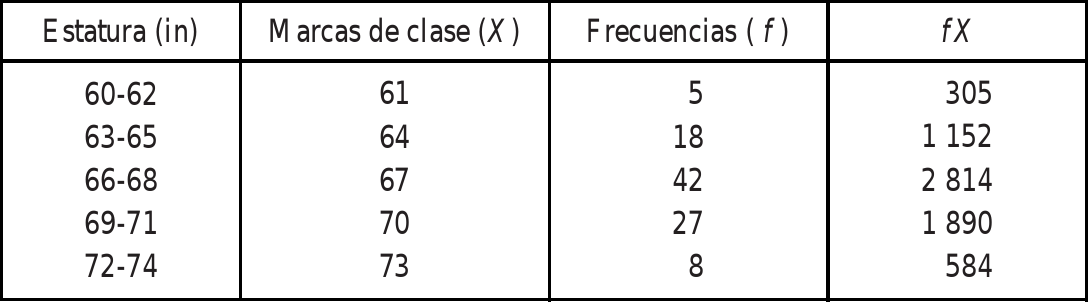
\includegraphics[width=10cm,keepaspectratio=true]{./images/tab0301.png}
		% tab0301.png: 0x0 pixel, 300dpi, 0.00x0.00 cm, bb=
		\label{tab:0301}
	\end{figure}
\end{problema}




\begin{problema}
	\label{problema:3.18}
	Si las desviaciones de $N$ números $X_{1},..,X_{N}$ respecto a un \emph{pivote} $P$ están dada por $d_{i}=X_{i}-P, \; i=1,...,N$ respectivamente, demostrar que
	\begin{align}
		\bar{X}=P+\dfrac{\sum d}{N}.
	\end{align}
\end{problema}



\begin{problema}
	\label{problema:3.16}
	Demostrar que la suma de las desviaciones $d_{1},d_{2},...,d_{N}$ de $X_{1},X_{2},...,X_{N}$ usando como pivote su media $\bar{X}$ es igual a cero.
\end{problema}



\begin{problema}
	\label{problema:3.17}
	Si $Z_{i}=X_{i}+Y_{i}, \; i=1,2,...,N,$ demostrar que $\bar{Z}=\bar{X}+\bar{Y}.$
\end{problema}




\begin{problema}
	\label{problema:3.19}
	Halle la media aritmética de los números 5,8,11,9,12,6,14 y 10 eligiendo como \emph{pivote} a) $P=9$ y b) $P=20.$
\end{problema}




\begin{problema}
	\label{problema:3.20}
	Utilice la marca de la clase media como pivote, para calcular la estatura de los estudiantes en la tabla \ref{tab:0301}.
\end{problema}



\begin{problema}
	\label{problema:3.28}
	Encontrar el peso mediano a partir de la siguiente tabla
	\begin{figure}[ht]
		\centering
		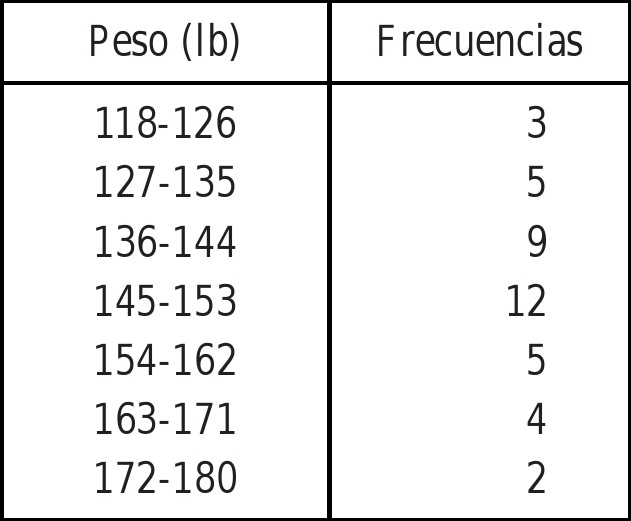
\includegraphics[height=5cm,keepaspectratio=true]{./images/tab0307.png}
		% tab0307.png: 0x0 pixel, 300dpi, 0.00x0.00 cm, bb=
		\label{tab:0307}
	\end{figure}
	
\end{problema}


\section{Medidas de dispersión}

\paragraph{Dispersión o variación}
Si bien las medidas de tendencia central nos dicen alrededor de que valores se concentra un arreglo de datos, las \emph{medidas de dispersión} nos dan una idea de que tan alejados están entre sí.





A continuación, veremos algunas medidas de dispersión comúnmente usadas en estadística.

\paragraph{Rango}
El \emph{rango}
de un conjunto de datos es la diferencia entre el mayor y el menor del conjunto.



\begin{ejemplo}
	El rango del conjunto 2,3,3,5,5,5,8,10,12 es $12-2=10.$
\end{ejemplo}


\paragraph{Desviación media}
La \emph{desviación media} o \emph{desviación promedio} de un conjunto de $N$ números $X_{1},...,X_{N}$ está definida como
\begin{align}
	DM=\dfrac{\sum \abs{X_{j}-\bar{X}}}{N}
\end{align}
donde $\bar{X}$ es la media aritmética de los números y $\abs{\cdot}$ denota el valor absoluto.


\begin{ejemplo}
	Encuentre la desviación media de la lista $2,3,6,8,11.$
\end{ejemplo}


\paragraph{Desviación estándar}
La \emph{desviación estándar} de un conjunto de $N$ números $X_{1},...,X_{N}$ se denota como $s$ y está definida por
\begin{align}
	s=\sqrt{\dfrac{\sum\left( X_{j}-\bar{X} \right)^{2}}{N}}=\sqrt{\sum\dfrac{x_{j}^{2}}{N}}
\end{align} donde $x_{j}:=X_{j}-\bar{X}.$


Si $X_{1},...,X_{N}$ se presentan con frecuencias $f_{1},...,f_{N}$ respectivamente, la desviación estándar se puede expresar como
\begin{align}
	s=\sqrt{\dfrac{\sum f_{j}\left( X_{j}-\bar{X} \right)^{2}}{N}}=\sqrt{\dfrac{\sum f_{j}x_{j}^{2}}{N}}
\end{align}


\begin{observacion}
	En ocasiones, $N$ se reemplaza por $N-1$ en las fórmulas anteriores, debido a que está definición aproxima mejor a la población de la que se ha obtenido la muestra. Pero para muestras muy grandes $N>30$ prácticamente no hay diferencia.
\end{observacion}


\paragraph{Varianza}
La \emph{varianza} de un conjunto de números se define como el cuadrado $s^{2}$ de la desviación estándar $s$.


\begin{observacion}
	En estadística, es importante distinguir entre la desviación estándar de una \emph{población} y una \emph{muestra}. Para distinguirla, en el primer caso utilizaremos $\s$ y en el segundo, continuaremos usando $s.$
\end{observacion}


\paragraph{Método abreviado}
\begin{align}
	s^{2}&=\overline{X^{2}}-\overline{X}^{2} \\
	&= E(X^2)-\left( E(X) \right)^{2}
	%\\ 
	%s^{2}&=\overline{d^{2}}-\overline{d}^{2}
\end{align}



En las distribuciones normales se tiene que
\begin{enumerate}
	\item $68.27\%$ de los datos está comprendido entre $\bar{X}\pm s.$
	\item $95.45\%$ de los datos está comprendido entre $\bar{X}\pm 2s.$
	\item $99.73\%$ de los datos está comprendido entre $\bar{X}\pm 3s.$
	
\end{enumerate}



Si $2$ conjuntos de $N_{1}$ y $N_{2}$ datos respectivamente tienen correspondientes $s_{1}^{2}$ y $s_{2}^{2}$ varianzas pero una misma media aritmética $\bar{X},$ entonces la varianza de la unión de ambos conjuntos es
\begin{align}
	s^{2}=\dfrac{N_{1}s_{1}^{2}+N_{2}s_{2}^{2}}{N_{1}+N_{2}}.
\end{align}

\paragraph{Teorema de Chebyshev}
Para $k>1,$ por lo menos $1-\dfrac{1}{k^{2}}$ de la distribución de problemaabilidad de cualquier variable aleatoria está a nomas  de $k$ desviaciones estándar de la media.

\subsection{Python}
[]{\texttt{numpy.std}}
\begin{lstlisting}[language=Python]
	numpy.std(a, axis=None, dtype=None, out=None, ddof=0,
	keepdims=<class numpy._globals._NoValue>)
\end{lstlisting}

Calcule la desviación estándar a lo largo del eje especificado.

Devuelve la desviación estándar, una medida de la propagación de una distribución, de los elementos de la matriz. La desviación estándar se calcula para la matriz aplanada de forma predeterminada, de lo contrario sobre el eje especificado.\footnote{https://docs.scipy.org/doc/numpy/reference/generated/numpy.std.html}

[]
\begin{lstlisting}[language=Python]
	import numpy as np
	
	a = np.array([[1, 2], [3, 4]])
	print np.std(a)
	#1.1180339887498949
	print np.std(a, axis=0)
	#array([ 1.,  1.])
	print np.std(a, axis=1)
	#array([ 0.5,  0.5])
\end{lstlisting}


[]
\begin{lstlisting}[language=Python]
	#In single precision, std() can be inaccurate:
	a = np.zeros((2, 512*512), dtype=np.float32)
	a[0, :] = 1.0
	a[1, :] = 0.1
	print np.std(a)
	#0.45000005
	
	#Computing the standard deviation in float64
	#is more accurate:
	print np.std(a, dtype=np.float64)
	#0.44999999925494177
\end{lstlisting}





\begin{problema}
	\label{problema:4.3}
	Encontrar el rango y las desviaciones media y estándar de los arreglos 
	\begin{enumerate}
		\item $12,6,7,3,15,10,18,5$ 
		\item $9,3,8,8,9,8,9,18.$
	\end{enumerate}
	
	Compruebe sus resultados con \texttt{Python.}
\end{problema}




\begin{problema}
	\label{problema:4.4}
	Encontrar las desviaciones media y estándar de las estaturas de 100 estudiantes de la siguiente tabla:
	\begin{figure}[ht]
		\centering
		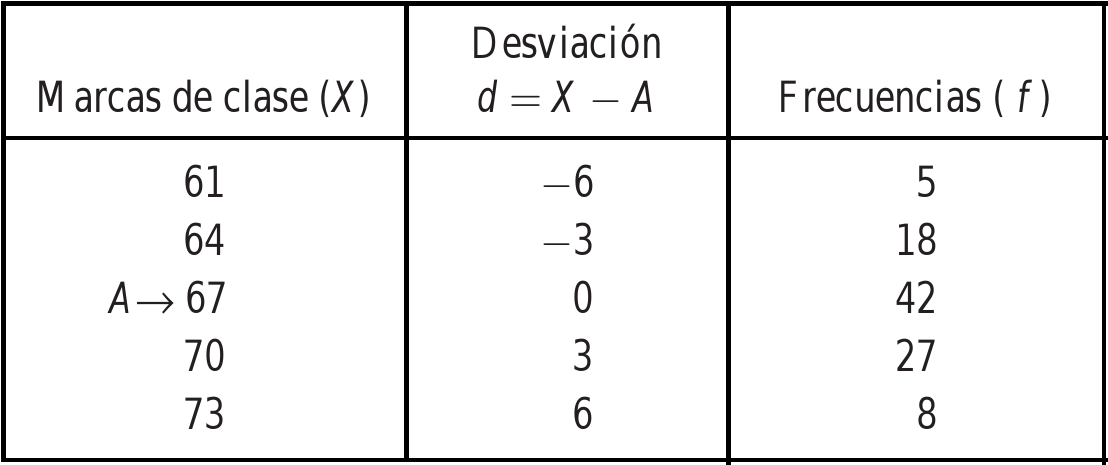
\includegraphics[width=10cm,keepaspectratio=true]{./images/tab0302.png}
		% tab0302.png: 0x0 pixel, 300dpi, 0.00x0.00 cm, bb=
		\label{tab:0302}
	\end{figure}
	
\end{problema}




\begin{problema}
	\label{problema:4.11}
	Encontrar las desviaciones media y estándar de las estaturas de 100 estudiantes de la siguiente tabla:
	\begin{figure}[ht]
		\centering
		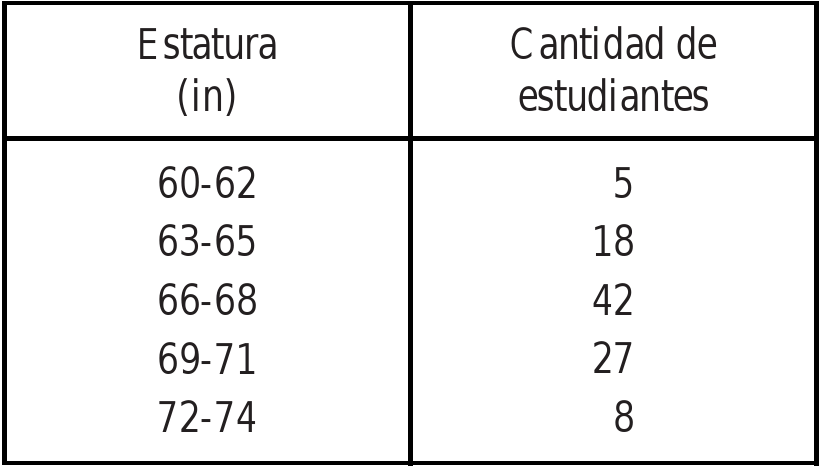
\includegraphics[height=5cm,keepaspectratio=true]{./images/tab0201.png}
		% tab0302.png: 0x0 pixel, 300dpi, 0.00x0.00 cm, bb=
		\label{tab:0201}
	\end{figure}
	
\end{problema}




\begin{problema}
	\label{problema:4.12}
	Demostrar que
	\begin{align}
		s &= \sqrt{\dfrac{\sum X^{2}}{N}-\left( \dfrac{\sum X}{N} \right)^{2}}&=
		\sqrt{\overline{X^{2}}-\overline{X}^{2}}\\
		s &= \sqrt{\dfrac{\sum fX^{2}}{N}-\left( \dfrac{\sum fX}{N} \right)^{2}}&=
		\sqrt{\overline{X^{2}}-\overline{X}^{2}}
	\end{align}
\end{problema}




\begin{problema}
	\label{problema:4.14}
	Utilizando las fórmulas anteriores, encuentre la desviación estándar de los datos en la tabla \ref{tab:0201}:
	\begin{figure}[ht]
		\centering
		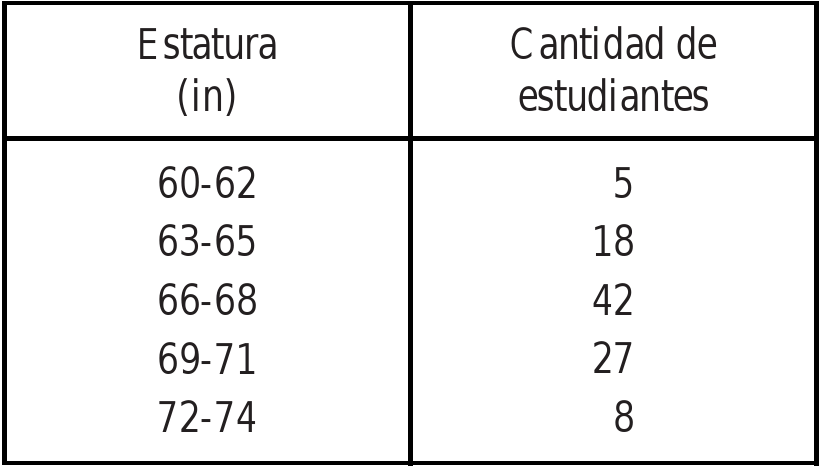
\includegraphics[height=5cm,keepaspectratio=true]{./images/tab0201.png}
		% tab0302.png: 0x0 pixel, 300dpi, 0.00x0.00 cm, bb=
		%\label{tab:0201}
	\end{figure}
	
\end{problema}




\begin{problema}
	\label{problema:4.15}
	Si $d=X-P$ son desviaciones de $X$ respecto a un pivote $P,$ demostrar que
	\begin{align}
		s=\sqrt{\dfrac{\sum fd^{2}}{N}-\left( \dfrac{\sum fd}{N} \right)^{2}}.
	\end{align}
\end{problema}



\begin{problema}
	\label{problema:4.17}
	Utilizando las fórmulas anteriores, encuentre la desviación estándar de los datos en la tabla \ref{tab:0201}:
	\begin{figure}[ht]
		\centering
		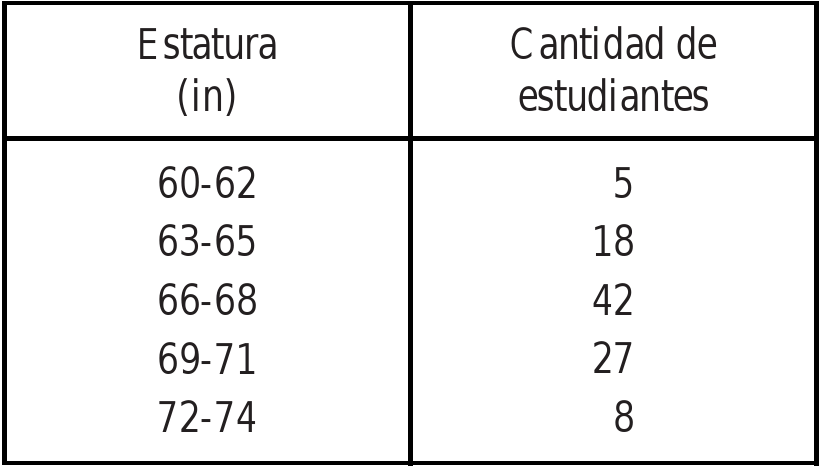
\includegraphics[height=5cm,keepaspectratio=true]{./images/tab0201.png}
		% tab0302.png: 0x0 pixel, 300dpi, 0.00x0.00 cm, bb=
		%\label{tab:0201}
	\end{figure}
	
\end{problema}




\begin{problema}
	\label{problema:4.18}
	Encuentre la media aritmética y  la desviación estándar de los siguientes datos:
	\begin{figure}[ht]
		\centering
		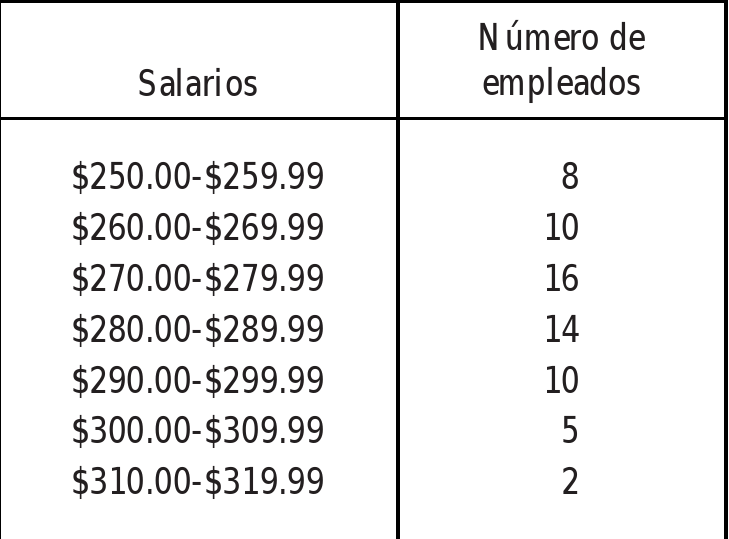
\includegraphics[height=5cm]{./images/tab0205.png}
		% tab0205.png: 0x0 pixel, 300dpi, 0.00x0.00 cm, bb=
		\label{tab:0205}
	\end{figure}
	
\end{problema}


%%%%%%%%%%%%%%%%%%%%%%%%%%%%%%
\chapter{Probabilidad}
\section{Notación de conjuntos}

\subsection{Introducción}

En esta actividad resolveremos problemas similares al de la figura \ref{fig:problema-conteo}.

\begin{figure}[h]
	\centering
	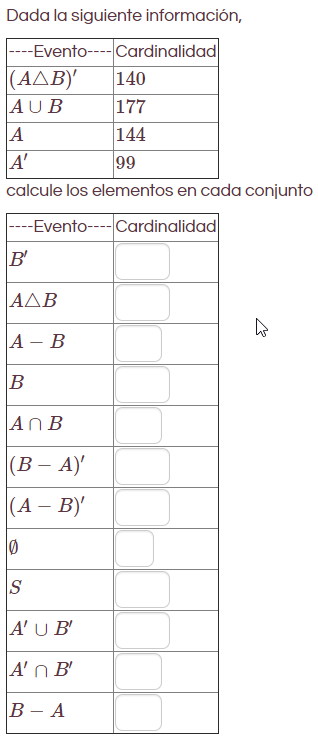
\includegraphics[width=0.7\linewidth]{images/2020-08-15 19_49_02}
	\caption{Problema de conteo}
	\label{fig:problema-conteo}
\end{figure}

Abordaremos el problema con el siguiente plan:
\begin{enumerate}
	\item Definir una partición en un conjunto.
	\item Fijar una partición estándar para describir las operaciones entre dos conjuntos. 
	\item Describir las operaciones entre conjuntos utilizando esta partición.
	\item Plantear y resolver el problema en términos de dicha partición. 
\end{enumerate}

Como prerrequisitos, se necesitarán conocer los siguientes conceptos:
\begin{enumerate}
	\item  Conjuntos y subconjuntos.
	\item Operaciones entre conjuntos.
	\item Solución de sistemas de ecuaciones lineales. 
\end{enumerate}

Para mayor claridad, recordaremos algunas definiciones de subconjuntos $ A,B \subset S $:
\begin{itemize}
	\item Unión
	\[ A\cup B = \sett{x\in S}{x \in A \texttt{ o } x \in B} \]
	\item Intersección
	\[ A\cap B = \sett{x \in S}{x\in A \texttt{ y } x\in B}\]
	\item Resta  
	\[ A\backslash B = \sett{x\in S}{x\in A \texttt{ y } x\not \in B}\]
	En ocasiones también denotamos la resta por $ A-B $. 
	\item Complemento
	\[ A' = \sett{x\in S}{x\not \in A} \]
	A veces el complemento también se denota por $ A^{c} $ o $ \bar{A} $. De manera equivalente, se puede escribir como $ S\backslash A.$
	\item Diferencia simétrica
	\[ A\triangle B = \sett{x \in S}{x\in A \texttt{ o } x\in B \texttt{ pero } x\not \in A\cap B}\]. 
\end{itemize}



\subsection{Particiones}

Consideremos un conjunto $ S $. Una partición (finita) es una colección $ \set{P_i \subset S}_{i=0}^{N}, N \in \N $ de subconjuntos de $ S $ que satisface
\begin{enumerate}
	\item $ P_i \cap P_j =\emptyset $ siempre que $ i\neq j $;
	\item $ \bigcup_{i=0}^{N} P_i = S $. 
\end{enumerate}

En otras palabras, son subconjuntos disjuntos entre sí que, al unirse todos, forman de nuevo el conjunto $ S $. El lector puede pensarlos como piezas de un rompecabezas.

\begin{figure}
	\centering
	
\includegraphics[width=0.7\linewidth]{images/puzzle-5294291_1280}
	\caption[Rompecabezas]{Los rompecabezas son ejemplos de particiones.}
	\label{fig:puzzle-52942911280}
\end{figure}

Consideremos dos conjuntos $ A,B \subset S$. El diagrama de Ven correspondiente esta dado por la figura \ref{fig:1280px-venndiagramforaunionb}. 

\begin{figure}
	\centering
	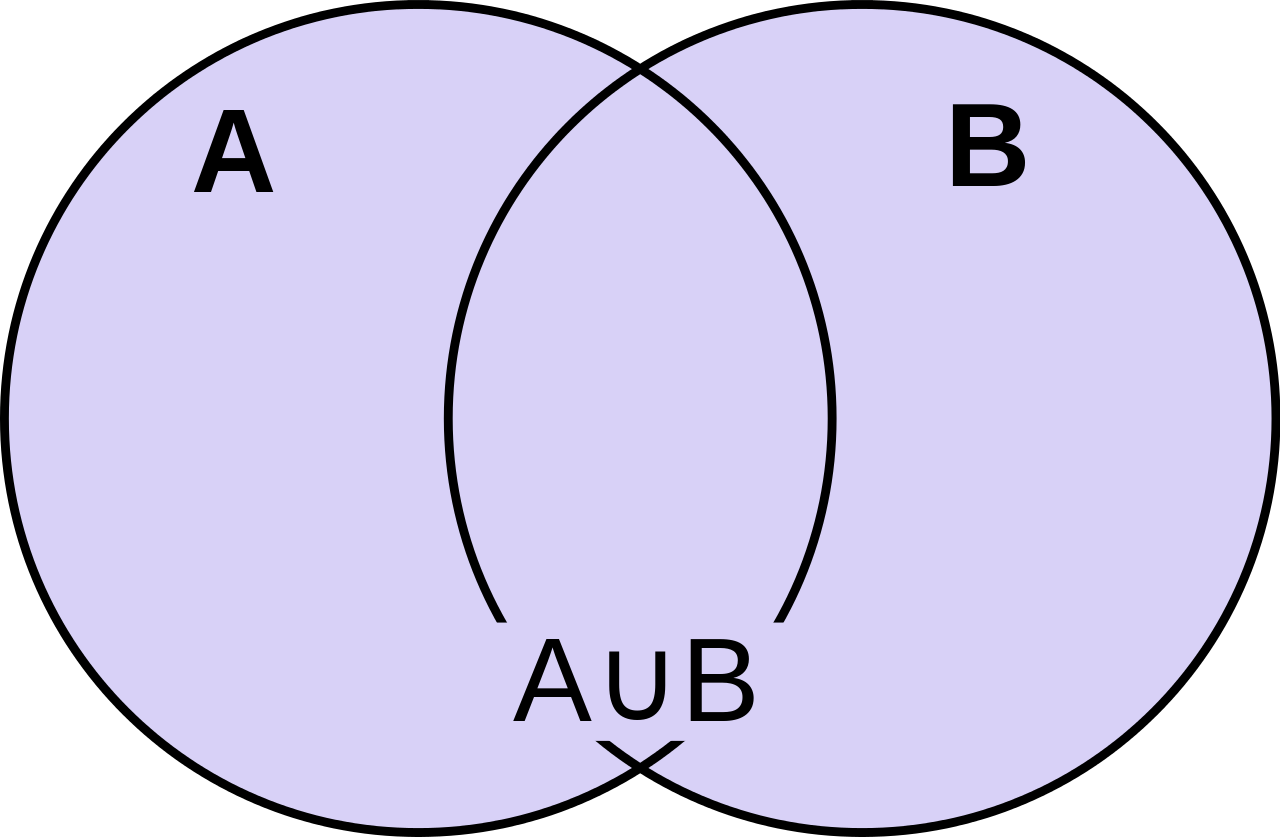
\includegraphics[width=0.7\linewidth]{images/1280px-Venn_diagram_for_A_union_B.svg}
	\caption{Diagram de Ven para dos conjuntos}
	\label{fig:1280px-venndiagramforaunionb}
\end{figure}

Entonces podemos definir una partición $ \particion(A,B) $ para $ S $ con los siguientes elementos
\begin{itemize}
	\item $ A\cap B $
	\item $ A\backslash B = A \cap B'$
	\item $ B\backslash A = B \cap A'$
	\item $ \left(A\cup B\right)' = A'\cap B' $
\end{itemize}

Para hacer la notación más concisa, definimos las siguientes aplicaciones:
\begin{align}
	\delta_C(x) = \begin{cases}
		1 & x \in C \\
		0 & x \not \in C
	\end{cases}
\end{align}
donde $ 1 $ denota \texttt{verdadero}, mientras que $ 0 $ denota \texttt{falso}, y
\begin{align}
	E_{(i,j)}=\sett{x\in S}{\delta_{A}(x)=i\wedge\delta_{B}(x)=j}
\end{align}
De manera que 
\begin{itemize}
	\item $ A' \cap B' = E_{(0,0)}$
	\item $ A'  \cap B = E_{(0,1)}$
	\item $ A \cap B'  = E_{(1,0)}$
	\item $ A  \cap B  = E_{(1,1)}$
\end{itemize}

Para hacer aún más sencilla la notación, identificaremos la pareja $ (i,j) $ con el correspondiente número binario $ [ij]_{2} $, convertido a base 10. De manera que 
\begin{itemize}
	\item $ A' \cap B' = E_{0}$
	\item $ A'  \cap B = E_{1}$
	\item $ A \cap B'  = E_{2}$
	\item $ A  \cap B  = E_{3}$
\end{itemize}

\subsection{Planteamiento del problema}

Como los elementos de un partición son disjuntos, entonces sabemos que 
\begin{align}
	\#\left(E_i\cup E_j\right) = \#E_i+\#E_j
\end{align}
siempre que $ i\neq j $.

Para simplificar la notación, definimos $ x_i=\# E_i. $

La primera ecuación que se nos plantea es
\begin{align}
	\left(A \triangle B \right)'=140,
\end{align}
donde 
\begin{align}
	A\triangle B = (A\backslash B)\cup(B\backslash A)
\end{align}
es la diferencia simétrica de $ A $ con $ B $. En otras palabras $ x\in A \triangle B $ si y solo si $ x\in A $ o $ x \in B $ pero no en ambos.

Observa que entonces
\begin{align}
	\label{ec01}
	\left(A\triangle B\right)' = E_0 \cup E_3 &
	\Rightarrow
	x_0 + x_3 = 140.
\end{align}

De manera similar, obtenemos las siguientes conclusiones:
\begin{align}
	\label{ec02}
	A\cup B = E_1\cup E_2 \cup E_3 &
	\Rightarrow x_1+x_2+x_3=177 \\
	\label{ec03}
	A = E_2 \cup E_3 &
	\Rightarrow x_2+x_3 = 144 \\
	\label{ec04}
	A' = E_0 \cup E_1 &
	\Rightarrow x_0+x_1 =99
\end{align}

Al resolver el sistema de ecuaciones dado por  \ref{ec01}-\ref{ec04}, obtenemos la solución:
\begin{align}
	x_0 &= 66 \\
	x_1 &= 33 \\
	x_2 &= 70 \\
	x_3 &= 74
\end{align}

\subsection{Solución del problema}

A continuación presentamos el desarrollo y conclusión de cada una de las preguntas en nuestro problema. Por ejemplo, podemos describir el complemento de $ B $ en términos de nuestra partición y utilizar las soluciones anteriores. 

\begin{align}
	\# B' 
	&= \#\left(E_1 \cup E_3\right)'\\
	&= \#\left(E_0 \cup E_2\right)\\
	&= x_0 + x_2 = 153
\end{align}

El resto de las soluciones se encuentras de la siguiente manera:

\begin{align}
	\card{A\triangle B} = x_1+x_2 = 103  \\
	\card{A\backslash B} = x_2 = 70 \\
	\card{B} = x_1+x_3=107	\\
	\card{A \cap B} = x_3 = 74 \\
	\card{\left(B\backslash A\right)'} 
	= x_0+x_2+x_3 = 210 \\
	\card{\left(A\backslash B\right)'}
	= x_0+x_1+x3 = 173 \\
	\card{\emptyset} = 0 \\
	\card{S} = x_0+x_1+x_2+x_3 = 243 \\
	\card{A' \cap B'} = x_0 = 66\\
	\card{B\backslash A} = x_1 = 33
\end{align}

Con esto concluimos nuestro ejercicio. 
\section*{Problemas}

\begin{problema}
	Extiende la construcción de una partición al caso de tres subconjuntos. 
\end{problema}
% teoría y ejemplos

\section{Fundamentos de probabilidad}

\subsection{Experimentos aleatorios}

\begin{ejemplo}
	\label{exmp:1.1}
	Si lanzamos una moneda, el resultado del experimento será reverso (\emph{tail} en inglés) que simbolizaremos con la letra "T" el número $0$ o anverso (\emph{head} en inglés) simbolizado por $H$ o $1$, es decir, uno de los elementos del conjunto $\set{T,H}$ (o bien $\set{0,1}.$)
\end{ejemplo}



\begin{ejemplo}
	\label{exmp:1.2}
	Si lanzamos un dado, el resultado del experimento resultará en uno de los números del conjunto $\set{1,2,3,4,5,6}.$
\end{ejemplo}



\begin{ejemplo}
	\label{exmp:1.3}
	Si lanzamos una moneda dos veces, existen cuatro posibles resultados:
	\begin{align}
		\set{HH,HT,TH,TT}.
	\end{align}
	
\end{ejemplo}



\begin{ejemplo}
	\label{exmp:1.4}
	Si estamos haciendo tornillos con una máquina, el resultado del experimento es que un tornillo puede salir defectuoso. Entonces cuando el tornillo este fabricado pertenecerá al conjunto
	\begin{align}
		\set{\texttt{defectuoso, no defectuoso}}
	\end{align}
	
\end{ejemplo}



\begin{ejemplo}
	\label{exmp:1.5}
	Si un experimento consiste en medir la \emph{vida útil} de una bombilla eléctrica producida por una compañía, entonces el resultado del experimento es tiempo $t$ medido en horas en algún intervalo
	\begin{align}
		0\leq t \leq T,
	\end{align}
	donde $T$ es el tiempo de vida máximo de una bombilla.
\end{ejemplo}



\subsection{El espacio muestral}
Un conjunto $S$ que consiste de todos los posibles resultados de un experimento aleatorio es llamado \emph{espacio muestral,}  y cada posible resultado es llamado un \emph{punto muestral.}

Usualmente existirá más de un espacio muestral que describe un experimento, pero elegiremos el que nos provee la mayor información.

\begin{ejemplo}
	\label{exmp:1.6}
	Si lanzamos un dado, un posible espacio muestral está dado por $\set{1,2,3,4,5,6},$  mientras que otro está dado por $\set{\text{par},\text{impar}}.$
\end{ejemplo}


\begin{ejemplo}
	\label{exmp:1.7}
	Si lanzamos una moneda dos veces seguidas un posible espacio muestral esta dado en el ejemplo \ref{exmp:1.3},  mientras que otro esta dado por
	\begin{align}
		\set{(0,0), (0,1), (1,0),(1,1)}.
	\end{align}
\end{ejemplo}



\begin{figure}
	\centering
	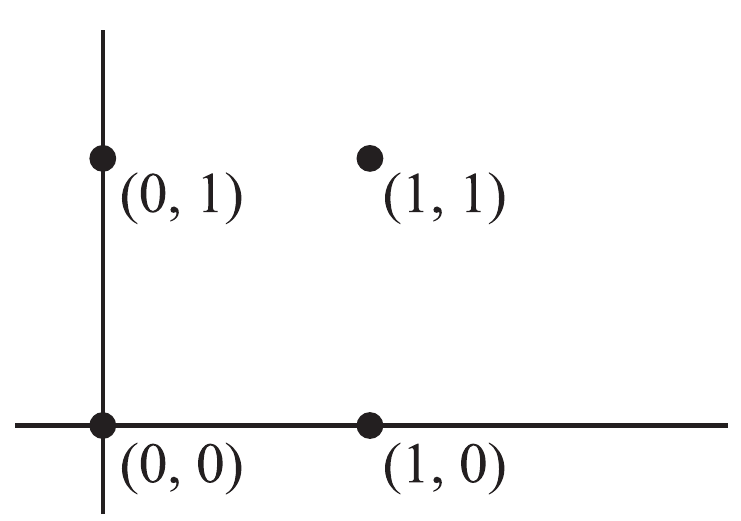
\includegraphics[width=5cm,keepaspectratio=true]{./pe/pands0101.png}
	% pands0101.png: 0x0 pixel, 300dpi, 0.00x0.00 cm, bb=
	\label{fig:0101}
\end{figure}


{Tipos de espacio muestral}
\begin{itemize}
	\item \emph{Finito:} tiene un número finito de puntos.
	\item \emph{Infinito numerable:} Tiene tantos puntos como los números naturales $\N$ (es decir, podemos numerar el espacio).
	\item \emph{Infinito no numerable:} Tiene tantos puntos como la recta real $\R.$  Por ejemplo, el intervalo $0<x<1.$
\end{itemize}



Si el espacio muestral es finito o infinito numerable, diremos que es \emph{discreto.}  Si es infinito no numerable, diremos que es \emph{continuo.}

\subsection{Eventos}

Un \emph{evento} es un subconjunto $A$ de un espacio muestral $S,$ es decir, un subconjunto de todos los posibles resultados de un experimento. Si el resultado es un elemento de $A,$ diremos que \emph{$A$ ha ocurrido.} 

Un evento que consiste de un único punto de $S$ es llamado a veces \emph{evento elemental o simple.}


\begin{figure}
	\centering
	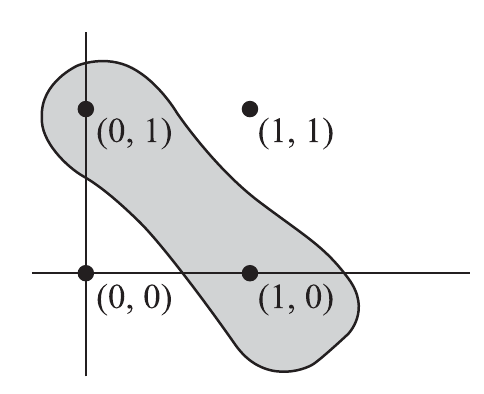
\includegraphics[height=3cm,keepaspectratio=true]{./pe/pands0102.png}
	% pands0102.png: 0x0 pixel, 300dpi, 0.00x0.00 cm, bb=
	\caption{Espacio muestral para el lanzamiento de una moneda dos veces seguidas.}
	\label{pands0102}
\end{figure}



\begin{ejemplo}
	\label{exmp:1.8}
	Si lanzamos una moneda dos veces, el evento de que obtengamos \emph{exactamente} un reverso  es un subconjunto del espacio muestral mostrado en la figura \ref{pands0102}.
\end{ejemplo}



Como eventos particulares, podemos considerar todo el espacio muestral $S$ como el \emph{evento cierto o seguro} y el conjunto vacío $\emptyset$ como el \emph{evento imposible.}


\subsection{Operaciones entre eventos} 
Supongamos que $A,B \subset S$ son dos eventos. 
\begin{itemize}
	\item $A\cup B$ es el evento \texttt{``ocurre $A$ o $B$ o ambos'',} y también es llamado \emph{unión de $A$ con $B$.}  
	\item $A\cap B$ es el evento \texttt{``ocurre $A$ y $B$'',} y también es llamado \emph{intersección de $A$ con $B$.}  
	\item $A'$ es el evento \texttt{``no ocurre $A$'',} y también es llamado \emph{negación de $A$.} 
	\item $A-B=A\cap B'$ es el evento \texttt{``ocurre $A$ pero no $B$'',} y también es llamado \emph{diferencia de $A$ menos $B.$}  Observe que
	$A' = S - A.$
\end{itemize}


Si $A\cap B= \emptyset,$ entonces diremos que \emph{$A$ y $B$} son \emph{disjuntos} o \emph{mutuamente excluyentes.} 

\begin{definicion}
	Si $A_{1},A_{2},... \subset S$ es una colección de eventos tales que $A_{i}\cap A_{j}=\emptyset$ siempre que $i\neq j,$ entonces diremos que son \emph{eventos mutuamente excluyentes}
\end{definicion}

\begin{definicion}
	Si $A_{1}, A_{2}, ...\subset S$ son eventos mutuamente excluyentes diremos que $A_{1} \cup A_{2} \cup ... $ es la \emph{unión disjunta} de tales eventos y en ese caso escribiremos
	\begin{align}
		A_{1}\sqcup A_{2} \sqcup ...
	\end{align}
\end{definicion}


\begin{definicion}
	Si \begin{align}
		S=A_{1}\sqcup A_{2} \sqcup ...
	\end{align}
	diremos que $A_{1},A_{2},...\subset S$  es una \emph{partición de $S.$}
\end{definicion}


\begin{ejemplo}
	\label{exmp:1.9}
	Respecto al experimentos de lanzar una moneda dos veces, consideremos el evento $A$ que consiste en \emph{obtener al menos un sol,}  mientras que el evento $B$ consiste en que \emph{el segundo lanzamiento sea un reverso.}
	
	Entonces $A=\set{TH,HT,HH},$ $B=\set{HT,TT}$ y por tanto 
	\begin{enumerate}
		\item $A\cup B =$ $\set{HT,TH,HH,TT}= S$ 
		\item $A\cap B =$ $\set{HT}$ 
		\item $A'=$$\set{TT}$
		\item $A-B=$$\set{TH,HH}$
	\end{enumerate}
	
\end{ejemplo}


\subsection{Enfoques de la probabilidad}

A cualquier evento en un espacio muestral se le puede asignar un número entre $0=0\%$ y $1=100\%$ que representa su \emph{probabilidad} de ocurrir.


Si un evento puede ocurrir en $h$ diferentes maneras de un total de $n$ posibles resultados, todos igualmente plausibles, entonces la probabilidad del evento es $h/n.$


\begin{ejemplo}
	\label{exmp:1.10}
	Supongamos que queremos conocer la probabilidad de que un sol aparezca en un solo volado.  Desde que hay dos maneras diferentes \emph{igualmente probables} en que la moneda caiga,  y de esas dos maneras un sol sólo puede hacerlo de una manera, razonamos que su probabilidad es $1/2.$
	
	
	\begin{observacion}
		Aquí suponemos que la moneda no está cargada.
	\end{observacion}
	
\end{ejemplo}


Si después de $n$ repeticiones de un experimento, donde $n$ es suficientemente grande, se observa que un evento ocurre en $h$ ocasiones, entonces diremos que la probabilidad del evento es $h/n.$  Esta es también llamada \emph{probabilidad empírica} del evento.


\begin{ejemplo}
	\label{exmp:1.11}
	Si lanzamos una moneda $1000$ veces y obtenemos sol 532 veces, estimamos que la probabilidad resultantes es $532/1000=0.532$.
\end{ejemplo}



\begin{observacion}
	Ambos enfoque tienen sus inconvenientes:
	\begin{enumerate}
		\item En el caso clásico, la expresión \emph{``igualmente probable''} es vaga; 
		\item mientras que en el enfoque frecuencial, \emph{``un número muy grande''} no es preciso. 
	\end{enumerate}
	Por estas razones, los matemáticos han desarrollado un \emph{enfoque axiomático} de la probabilidad.
\end{observacion}


\subsection{Los Axiomas de la probabilidad}

Supongamos que tenemos un espacio muestral $S.$ Supongamos que $C$ es la colección de todos los eventos en $S.$ Diremos que $P:C \to \R$ es una función de probabilidad si satisface las siguientes propiedades:

\begin{axioma}
	Para cada evento $A,$ se tiene que
	\begin{align}
		\label{1.1}
		P(A)\geq 0.
	\end{align}
	
\end{axioma}



\begin{axioma}
	La probabilidad del evento cierto $S$ es
	\begin{align}
		\label{1.2}
		P(S)=1.
	\end{align}
\end{axioma}



\begin{axioma}
	Para cualquier cantidad numerable de eventos mutuamente excluyentes
	$A_{1},A_{2},...$ tenemos que
	\begin{align}
		\label{1.3}
		P(A_{1}\sqcup A_{2} \sqcup ...)=P(A_{1})+P(A_{2})+...
	\end{align}
	En particular, para dos eventos mutuamente excluyentes $A_{1},A_{2},$
	\begin{align}
		\label{1.4}
		P(A_{1}\sqcup A_{2})=P(A_{1})+P(A_{2})
	\end{align}
	
\end{axioma}


\subsection{Algunos teoremas importantes en probabilidad}

\begin{teorema}
	\label{thm:1.1}
	Si $A_{1}\subset A_{2},$ entonces $P(A_{1})\leq P(A_{2})$ y
	\begin{align}
		P(A_{2}-A_{1})=P(A_{2})-P(A_{1}).
	\end{align}
\end{teorema}


\begin{teorema}
	\label{thm:1.2}
	Para cada evento $A$,
	\begin{align}
		\label{1.5}
		0\leq P(A) \leq 1,
	\end{align}
	
	es decir, la probabilidad siempre se encuentra entre $0\%$ y $100\%.$
\end{teorema}


\begin{teorema}
	\label{thm:1.3}
	El evento imposible tiene probabilidad cero, es decir,
	\begin{align}
		P(\emptyset)=0.
	\end{align}
\end{teorema}


\begin{teorema}
	\label{thm:1.4} La probabilidad de un evento complementarios está dada por
	\begin{align}
		\label{1.7}
		P(A')=1-P(A)
	\end{align}
\end{teorema}


\begin{teorema}
	\label{thm:1.5} Si $A=A_{1}\sqcup...\sqcup A_{N}$ es la unión disjunta de eventos mutuamente excluyentes entonces
	\begin{align}
		\label{1.8}
		P(A)=P(A_{1})+...+P(A_{N}).
	\end{align}
	
	
	En particular, si $S=A_{1}\sqcup...\sqcup A_{N}$ entonces
	\begin{align}
		\label{1.9}
		P(A_{1})+...+P(A_{N})=1.
	\end{align}
\end{teorema}


\begin{teorema}
	\label{thm:1.6}
	Si $A,B,C$ son dos eventos no necesariamente excluyentes, entonces
	\begin{align}
		\label{1.10}
		P(A\cup B)=P(A)+P(B)-P(A\cap B).
	\end{align}
	\begin{align}
		\label{1.11}
		P(A\cup B \cup C)&=P(A)+P(B)+P(C)\\
		&-P(A\cap B)-P(B\cap C)-P(C\cap A)\\
		&+P(A\cup B \cup C).
	\end{align}
\end{teorema}



\begin{teorema}
	\label{thm:1.7}
	Para cualesquiera eventos $A,B,$
	\begin{align}
		\label{1.12}
		P(A)=P(A\cap B)+P(A\cap B').
	\end{align}
\end{teorema}


\begin{teorema}
	\label{thm:1.8}
	Si $A_{1},A_{2},..., A_{N}$ es una partición del espacio muestral $S,$ es decir,
	$S=A_{1} \sqcup A_{2} \sqcup ... \sqcup A_{N}$ entonces para cualquier evento $A$
	\begin{align}
		\label{1.13}
		P(A)=P(A\cap A_{1})+ P(A\cap A_{2}) + ... +P(A\cap A_{N}).
	\end{align}
\end{teorema}


\subsection{Asignación de probabilidades}

Si un espacio muestral consiste en una cantidad \emph{finita} de posibles resultados $a_{1},...,a_{N},$ entonces por el teorema \ref{thm:1.5},
\begin{align}
	\label{1.14}
	P(A_{1})+...+P(A_{n})=1
\end{align}
donde $A_{1},...,A_{n}$ son \emph{conjuntos elementales} o \emph{eventos simples} dados por $A_{i}=\set{a_{i}}.$


Se sigue que uno puede escoger de manera arbitraria cualesquiera números no negativos como probabilidades de estos eventos simples, siempre que se satisfaga \eqref{1.14}. 

En particular, si suponemos \emph{probabilidades iguales} para todos los eventos, entonces
\begin{align}
	\label{1.15}
	P(A_{k})=\dfrac{1}{n}, \; k=1,2,...,n,
\end{align}
y si $A$ es un evento formado por la unión disjunta de $h$ eventos simples, entonces
\begin{align}
	\label{1.16}
	P(A)=\dfrac{h}{n}.
\end{align}


\begin{observacion}
	Esto es equivalente al \textit{enfoque clásico.} Pero podemos usar el \textit{enfoque frecuencial} para asignar dichas probabilidades.
\end{observacion}


\begin{ejemplo}
	\label{exmp:1.12}
	Si solo dado se lanza, la probabilidad de que obtengamos un 2 o un 5 es 
	\[ P(\set{2,5}) = P(\set{2}) + P(\{5\}) = 1/6 + 1/6 = 1/3. \]
\end{ejemplo}

% problemas: fundamentos de probabilidad

\section*{Problemas}

La baraja está dividida en cuatro palos (en inglés: suit), dos de color rojo y dos de color negro:
\begin{itemize}
	\item Espadas (conocidas como picas) $\spadesuit$,
	\item Corazones $\heartsuit$,
	\item Rombos (conocidos como diamantes, oros o cocos) $ \diamondsuit$,
	\item Tréboles (conocidos como flores) $\clubsuit$
\end{itemize}

Cada palo está formado por 13 cartas, de las cuales 9 cartas son numerales y 4 literales. Se ordenan de menor a mayor "rango" de la siguiente forma: A, 2, 3, 4, 5, 6, 7, 8, 9, 10, J, Q y K.

\begin{figure}
	\centering
	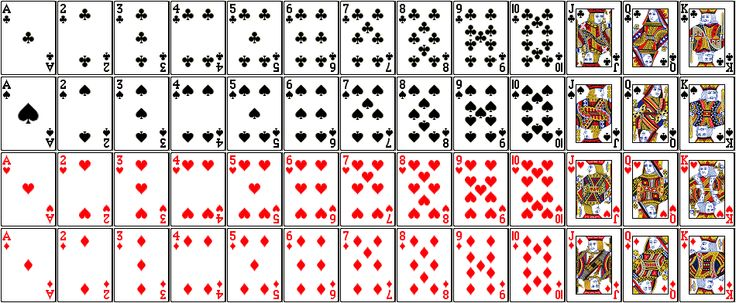
\includegraphics[width=10cm]{./pe/deck.jpg}
	% deck.jpg: 0x0 pixel, 300dpi, 0.00x0.00 cm, bb=
	\caption{Baraja inglesa}
	\label{fig:deck}
\end{figure}



\begin{problema}
	\label{problema:2.1}
	Una carta se obtiene al azar de una baraja inglesa. Describe el espacio muestral si se consideran los palos.
\end{problema}

\begin{solucion}\label{solucion:2.1}
	
	\href{https://youtu.be/4LdLWpQIcBQ}{Consulta también la solución en línea.}
	
	
	La solución está dada por el producto cartesiano del conjunto \[ A = \set{1,2,3,4}, \] donde cada número representa alguno de los palos, y el conjunto \[ B = \set{A,2,...,10,J,Q,K}.\] De manera que el espacio muestral contiene $ 4\times 13=52 $ puntos muestrales. 	
\end{solucion}


\begin{problema}
	\label{problema:2.2}
	Supongamos que $A$ es el evento \texttt{``se obtiene un rey''} o simplemente $\set{K},$ mientras que $B$ es \texttt{``se obtiene un tr\'ebol} o simplemente $\set{\clubsuit}$. Describe los siguiente eventos: 
	\begin{enumerate}
		\item $A\cup B$ 
		\item $A\cap B$ 
		\item $A \cup B'$ 
		\item $A' \cup B'$ 
		\item $A - B$ 
		\item $A'-B'$ 
		\item $(A\cap B) \cup (A\cap B')$
	\end{enumerate}
\end{problema}

\begin{solucion}
	\label{solucion:2.2}
	\href{https://youtu.be/S9VFhMWVyu4}{Consulta también la solución en línea.}
	\begin{enumerate}
		\item Se obtiene un rey o un trébol.
		\item Se obtiene un rey y un trébol.
		\item Se obtiene un rey o no se obtiene un trébol. De manera equivalente: Si se obtiene un trébol, entonces se obtiene un rey. 
		\item No se obtiene un rey o no se obtiene un trébol.
		\item Se obtiene un rey, pero no un trébol. 
		\item No se obtiene un rey ni un trébol.
		\item O bien se obtiene un rey y un trébol, o bien se obtiene un rey pero no un trébol. De manera equivalente: Se obtiene un rey.		
	\end{enumerate}
\end{solucion}



\begin{problema}
	\label{problema:2.3}
	De una baraja inglesa se extraen 2 cartas. Encuentre la probabilidad de que las dos sean ases si la primera carta...
	\begin{enumerate}
		\item ...se devuelve a la baraja.
		\item ...no se devuelve a la baraja.
	\end{enumerate}
	
\end{problema}

\begin{solucion}
	\label{solucion:2.3}
	\begin{enumerate}
		\item \[ \dfrac{4}{52}\times\dfrac{4}{52} = \dfrac{1}{13}\times \dfrac{1}{13} = \dfrac{1}{169} \]
		\item \[ \dfrac{4}{52}\times\dfrac{3}{51} = \dfrac{1}{221} \]
	\end{enumerate}
\end{solucion}


\begin{problema}
	\label{problema:2.4}
	En un contenedor hay 6 pelotas rojas, 4 blancas y 5 azules. Se extraen sucesivamente 3 pelotas. Encuéntrese la probabilidad de que se extraigan en el orden roja, blanca y azul si...
	\begin{enumerate}
		\item ...cada pelota se devuelve a la caja.
		\item ...no se devuelve.
	\end{enumerate}
	
\end{problema}

\begin{solucion}
	\label{solucion:2.4}
	En total, hay 15 pelotas en el contenedor.
	\begin{enumerate}
		\item 
		\[
			\dfrac{6}{15}\times\dfrac{4}{15}\times\dfrac{5}{15}
			=\dfrac{8}{225}.
		\]
	\item
	\[
		\dfrac{6}{15}\times\dfrac{4}{14}\times\dfrac{5}{13}
		=\dfrac{4}{91}.
	\]
	\end{enumerate}
\end{solucion}


\begin{problema}
	\label{problema:2.5}
	Encuéntrese la probabilidad de que en dos lanzamientos de un dado se obtengan por lo menos un 4 en alguno de los dos lanzamientos.
\end{problema}

\begin{solucion}
	\label{solucion:2.5}
	El espacio solución está dado por 
	\[
		E = \set{4,5,6}\times \set{1,..,6} \cup \set{1,...,6}\times\set{4,...,6}
	\]
cuya cardinalidad es $ 9 $. 

Ahora bien, el espacio muestral está dado por
\[
	S = \set{1,...,6}\times\set{1,...,6},
\]
cuya cardinalidad es $ 36 $.

De manera que la probabilidad es 
\[
	\dfrac{9}{36}=\dfrac{1}{4}.
\]

\end{solucion}

\begin{problema}
	\label{problema:2.6}
	Encuentre la probabilidad de no obtener una suma de 7 o de 11 puntos al lanzar ambos dados.
\end{problema}


\begin{solucion}
	\label{solucion:2.6}
	Consideremos nuevamente el espacio muestral 
	\[
		S = \set{1,...,6}\times\set{1,...,6}.
	\]

	Podemos obtener una suma igual con 7 con los siguientes puntos:
	\[
		\set{(1,6),(2,5),(3,4),(4,3),(5,2),(6,1)}, 
	\]
	mientras que la de 11, con los siguientes:
	\[\label{key}
		\set{(5,6), (6,5)}
	\].

	Estos eventos son mutuamente excluyentes (es decir, como conjuntos son disjuntos). Por lo que existen 8 posibles eventos simples con los que obtendríamos o bien una suma de 7 o bien una suma de 11.
	
	Por tanto, la probabilidad es
	\[\label{key}
		1-\dfrac{11}{36}=\dfrac{25}{36}.
	\]
\end{solucion}
 \section{Probabilidad condicional}
{}
Sean $A,B$ dos eventos tales que $P(A)>0.$
\begin{figure}
	\centering
	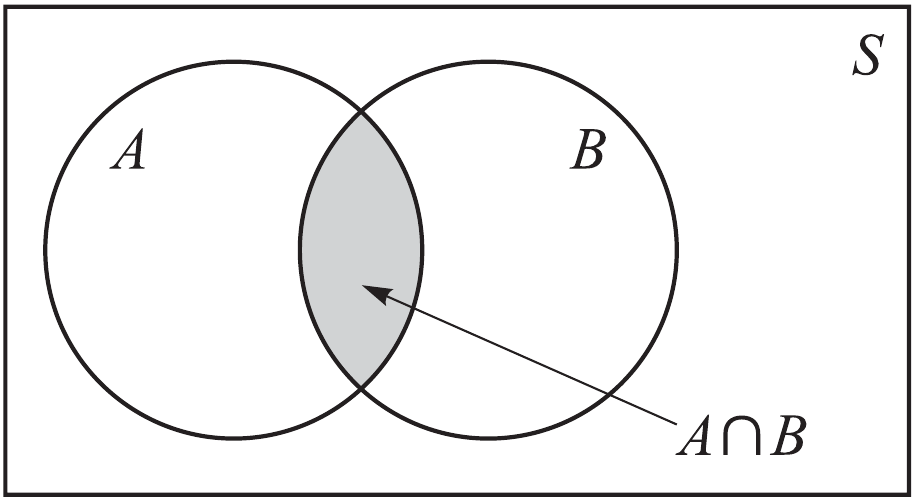
\includegraphics[width=5cm,keepaspectratio=true]{./pe/pands0103.png}
	% pands0103.png: 0x0 pixel, 300dpi, 0.00x0.00 cm, bb=
	\label{pands0103}
\end{figure}

Denotaremos por $P(B|A)$
la probabilidad de $B$ dado que $A$ haya ocurrido y diremos que es la \emph{probabilidad condicional} de $B$ dado $A.$


\begin{definicion}[Probabilidad condicional]
	\begin{align}
		P(B|A)&=\dfrac{P(A\cap B)}{P(A)} \\
		P(A\cap B) &= P(A)P(B|A)
	\end{align}
\end{definicion}


{}
\begin{observacion}
	La probabilidad condicional satisface todos los axiomas de una función de probabilidad.  Podemos pensar $P(\cdot|A)$ como la función de probabilidad que se obtiene al reemplazar el espacio muestral $S$ por $A.$
\end{observacion}


{}
\begin{ejemplo}
	\label{exmp:1.13}
	Encontrar la probabilidad de que una solo lanzamiento de un dado resulte en un número menor que $4$ si
	\begin{enumerate}
		\item no hay más información; 
		\item se sabe que el lanzamiento resultó en un número impar.
	\end{enumerate}
	
\end{ejemplo}


{}
\begin{teorema}
	\label{thm:1.9}
	Para cualesquiera tres eventos $A_{1},A_{2},A_{3},$ tenemos que
	\begin{align}
		\label{1.19}
		P(A_{1} \cap A_{2} \cap A_{3})=P(A_{1})P(A_{2}|A_{1})P(A_{3}|A_{1} \cap A_{2})
	\end{align}
\end{teorema}


{}
\begin{teorema}
	\label{thm:1.10} Si $S=A_{1}\sqcup ... \sqcup A_{N},$  entonces
	\begin{align}
		\label{1.20}
		P(A)=P(A_{1})P(A|A_{1})+...+P(A_{N})P(A|A_{N})
	\end{align}
\end{teorema}


{}
Si $P(B|A)=P(B),$ i.e., la probabilidad de que $B$ ocurra no está afectada por la ocurrencia de $A,$ entonces diremos que $A$ y $B$ son independientes.


\begin{definicion}
	$A$ y $B$ son eventos independientes si y solo si
	\begin{align}
		\label{1.21}
		P(A \cap B) = P(A)P(B).
	\end{align}
\end{definicion}


{}
La definición se puede generalizar a más de dos eventos.  Por ejemplo, diremos que $A_{1},A_{2},A_{3}$ son eventos independientes si
\begin{align}
	k\neq j \rightarrow P(A_{j} \cap A_{k})=P(A_{j})P(A_{k}), \; j,k=1,2,3 
	\\ P(A_{1}\cap A_{2} \cap A_{3})=P(A_{1})P(A_{2})P(A_{3}).
\end{align}


\begin{teorema}[Teorema de Bayes]
	Si $S=A_{1}\sqcup A_{2} \sqcup...\sqcup A_{N},$ entonces
	\begin{align}
		\label{1.24}
		P(A_{k}|A) = \dfrac{P(A_{k})P(A|A_{k})}{\sum_{j} P(A_{j})P(A|A_{j})}
	\end{align}
	
\end{teorema}





%\section*{Problemas}


\begin{problema}
	\label{solved:1.16}
	Demuestre el teorema de Bayes.
\end{problema}



{}
\begin{problema}
	\label{solved:1.15}
	La caja $I$ contiene 3 canicas rojas y 2 azules, mientras que la caja $II$ contiene $8$ canicas rojas y 8 azules. Una moneda se lanza: Si cae un sol, se escoge una moneda de la caja $I$ y si cae reverso, de la caja $II.$ Encuentre la probabilidad de obtener una canica roja.
\end{problema}


{}
\begin{problema}
	\label{solved:17}
	Supongamos que en el problema anterior, quien lanza la moneda no revela si ha caído reverso o sol (de manera que la caja de la que se obtiene la canica no se revela) pero revela que una canica roja se ha obtenido.?`Cual es la probabilidad de haber obtenido un sol?
\end{problema}
\section{Teorema de Bayes}

Si tanto $ P(A) $ como $ P(B) $ son diferentes de cero, entonces, a partir de la definición de probabilidad condicional, podemos deducir que 
\begin{align}
	P(A \cap B) &=P(A)\cdot P(B|A)\\
	P(B \cap A) &=P(B)\cdot P(A|B),
\end{align}
y como $ P(A\cap B)= P(B\cap A) $, concluimos 
\begin{align}
	P(A)\cdot P(B|A) = P(B)\cdot P(A|B)
\end{align}
y por tanto 
\begin{align}
	P(A|B)=\dfrac{P(A)\cdot P(B|A)}{P(B)}.
\end{align}
El resultado es conocido como \emph{teorema de Bayes.}

\subsection{Generalizaciones}

El resultado anterior se puede extender de la siguiente manera: Como 
\begin{align}
	\begin{cases}
		(B\cap A) \cup (B \cap A') &= B\\
		(B\cap A) \cap (B \cap A') &= \emptyset\\
	\end{cases},
\end{align}
entonces
\begin{align}
	P(B) & = P\left( (B\cap A) \cup (B \cap A') \right)\\
	&= P(B\cap A) + P(B\cap A')\\
	&= P(B|A)P(A) + P(B|A')P(A'),
\end{align}
de manera que 
\begin{align}
	P(A|B)=\dfrac{P(A)\cdot P(B|A)}{P(B|A)P(A) + P(B|A')P(A')}.
\end{align}

Podemos generalizar este concepto usando una partición $ \seq{E_i}{i=0}{N} $ del espacio muestral $ S \supset A, B$. En ese caso
\begin{align}
	A = \bigcup_{i=0}^{N}(A\cap E_i)
\end{align}
y por tanto
\begin{align}
	P(B) &= \sum_{i=0}^{N} P(B\cap E_i)\\
	&= \sum_{i=0}^{N} P(B|E_i)P(E_i).
\end{align}
A este resultado lo llamaremos \emph{regla de la cadena.}

Ahora bien, de manera similar al primer caso del teorema de Bayes, concluímos que 
\begin{align}
	P(B|E_j)P(E_j)= P(E_j|B)P(B),
\end{align}
de forma que utilizando la regla de la cadena, obtenemos
\begin{align}
	P(E_j|B)&= \dfrac{P(B|E_j)P(E_j)}{P(B)}\\
	&=\dfrac{P(B|E_j)P(E_j)}{\sum_{i=0}^{N} P(B|E_i)P(E_i)}
\end{align}

\begin{ejemplo}
	Una planta productora de gelatinas cuenta con tres máquinas empacadoras. Así la distribución de volumen de empaque se realiza de la siguiente manera:
	\begin{itemize}
		\item Máquina 1: 38\%
		\item Máquina 2: 32\%
		\item Máquina 3: 30\%
	\end{itemize}
	
	De esta manera, la probabilidad de que el empaque salga defectuoso es de 11\%, 15\% y 14\%, respectivamente por cada máquina. 
	
	La gerencia de producción de la planta está interesada en conocer cuál es la probabilidad de que si se selecciona una unidad al azar y es defectuoso, esta se haya empacado en la máquina 2. 

	Denotemos por $ M_i $ el evento de que una unidad de gelatina se haya empacado en la $ i $-ésima máquina, mientras que $ D $ es el evento de que la unidad sea defectuosa. 
	
	De acuerdo al problema 
	\begin{align}
		P(M_1)&=0.38\\
		P(M_2)&=0.32\\
		P(M_3)&=0.30\\
		P(D|M_1)&=0.11\\
		P(D|M_2)&=0.15\\
		P(D|M_3)&=0.14
	\end{align}
	
	Entonces 
	\begin{align}
		P(M_2|D) &= \dfrac{P(D|M_2)P(M_2)}{	P(D|M_1)P(M_1)+P(D|M_2)P(M_2)+P(D|M_3)P(M_3)
		}\\
		&= \dfrac{(0.15)(0.32)}{
			(0.11)(0.38)+(0.15)(0.32)+(0.14)(0.30)	
		}\\
		&=0.3642=36.42\%
	\end{align}
\end{ejemplo}
\section*{Problemas}

\begin{problema}
	\label{bayes-pro-1}
	\sidenote{\href{https://stempunkxyz.wordpress.com/2021/08/02/teorema-de-bayes-1/}{Solución al problema \ref{bayes-pro-1}}}
	\label{exmp:1.13}
	Encontrar la probabilidad de que una solo lanzamiento de un dado resulte en un número menor que $4$ si
	\begin{enumerate}
		\item no hay más información; 
		\item se sabe que el lanzamiento resultó en un número impar.
	\end{enumerate}
	
\end{problema}


\begin{problema}
	%schaum solved 1.15, 1.17
	\begin{enumerate}
		\item 
		La caja 1 contiene 3 canicas rojas y 2 azules, mientras que la caja 2 contiene 2 canicas rojas y 8 azules. 
		
		Se lanzan dos dados y se calcula la suma:  
		Si se obtiene una suma de a lo más seis puntos, se elige una canica de la caja I; en otro caso, se elige una canica de la caja 2. 
		
		Calcula la probabilidad de que se elija una canica roja.
		\item Supongamos que quien lanza la moneda no revela si que número se obtuvo del dado, pero sí revela que se eligió una canica roja. ¿Cuál es la probabilidad de que se eligiera la caja 1?
	\end{enumerate}
\end{problema}

%\begin{problema}
%	%wackerly ejemplo 2.23
%	Un fusible electrónico es producido por cinco líneas de producción en una operación de manufactura. Los fusibles son costosos, sumamente confiables y se envían a proveedores en lotes de 100 unidades. 
%	
%	Como la prueba es destructiva, la mayoría de los compradores de fusibles prueban solo un número pequeño de ellos antes de decidirse a aceptar o rechazar lotes de fusibles que lleguen.
%	
%	Las cinco líneas de producción producen fusibles al mismo ritmo y normalmente producen solo 2\% de fusibles defectuosos, que se dispersan al azar en la producción. 
%	
%	Desafortunadamente, la línea 1 de producción sufrió problemas mecánicos y produjo 5\% de piezas defectuosas durante el mes de marzo. 
%	
%	Esta situación llegó al conocimiento del fabricante después de que los fusibles ya habían sido enviados. Un cliente recibió un lote producido en marzo y probó tres fusibles. Uno falló. 
%	
%	\begin{enumerate}
%		\item 
%		¿Cuál es la probabilidad de que el lote se haya producido en la línea 1? 
%		\item ¿Cuál es la
%		probabilidad de que el lote haya provenido de una de las otras cuatro líneas?
%	\end{enumerate}
%\end{problema}

\section{Variables aleatorias discretas}

Supongamos que a cada punto del espacio muestral se le asigna un número.  Entonces hemos definido una \emph{función} en el espacio muestral  Esta función es llamada \emph{variable aleatoria} (o \emph{variable estocástica}) o de manera más precisa \emph{función aleatoria}. 


Usualmente, las variables aleatorias se denotan por letras mayúsculas como $X$ o $Y$. En general, una variable aleatoria tiene algún significado físico, geométrico, económico, financieros, etc.



\begin{ejemplo}
	\label{exmp:2.1}
	Supongamos que una moneda se lanza dos veces de manera que el espacio muestral es $\set{HH,HT,TH,TT}.$  Digamos que $X$ representa el número de soles ($H$) que obtenemos.
\end{ejemplo}


\subsection{Funciones de probabilidad discretas}

Sea $X$ una variable aleatoria discreta.  Supongamos que los valores que puede tomar son $x_{1},...,x_{k},$ arreglados en algún orden dado.  Supongamos también que esos valores
tienen alguna probabilidad dada por
\begin{align}
	\label{2.1}
	P(X=x_{k})=f(x_{k}).
\end{align}


{Función de probabilidad}
\begin{align}
	\label{2.2}
	P(X=x)=
	\begin{cases}
		f(x) & x=x_{k} \\
		0	& \text{en otro caso}
	\end{cases}
\end{align}



En general, $f(x)$ será una función de probabilidad si
\begin{align}
	\begin{cases}
		f(x)\geq 0 \\
		\sum_{x}f(x)=1.
	\end{cases}
\end{align}



\begin{ejemplo}
	\label{exmp:2.2}
	Encuentre la función de probabilidad correspondiente a la variable aleatoria $X$ del ejemplo \ref{exmp:2.1}.
\end{ejemplo}



\begin{ejemplo}
	\label{sol:2.1}
	Suponga que un par de dados se lanzan. Sea $X$ la variable aleatoria dada por la suma de los puntos. Encuentre la distribución de probabilidad de $X.$
\end{ejemplo}



\begin{ejemplo}
	\label{sol:2.2}
	Encuentre la distribución de probabilidad de niños y niñas en familias con 3 hijos, suponiendo la misma probabilidad para niños y niñas.
\end{ejemplo}



\subsection{Funciones de distribución para variables aleatorias discretas}


La función de distribución de una variable discreta $X$ se obtiene de la función de probabilidad a través de la siguiente fórmula
\begin{align}
	\label{2.4}
	F(x) = P(X\leq x) = \sum_{u \leq x} f(u).
\end{align}



Si $X$ toma sólo un número finito de valores $x_{1},...,x_{n}$ entonces la función de distribución está dada por
\begin{align}
	\label{2.5}
	F(x)=
	\begin{cases}
		0 & -\infty < x < 0 \\
		f(x_{1}) & x_{1} \leq x < x_{2} \\
		f(x_{1})+f(x_{2}) & x_{2} \leq x < x_{3} \\
		\vdots & \vdots \\
		f(x_{1})+\cdots+f(x_{n}) & x_{n} \leq x < \infty
	\end{cases}
\end{align}



\begin{ejemplo}
	\label{exmp:2.3}
	Encuentre la función de distribución para la variable aleatoria $X$ del ejemplo \ref{exmp:2.2} y obtenga su gráfica.
\end{ejemplo}



\begin{figure}
	\centering
	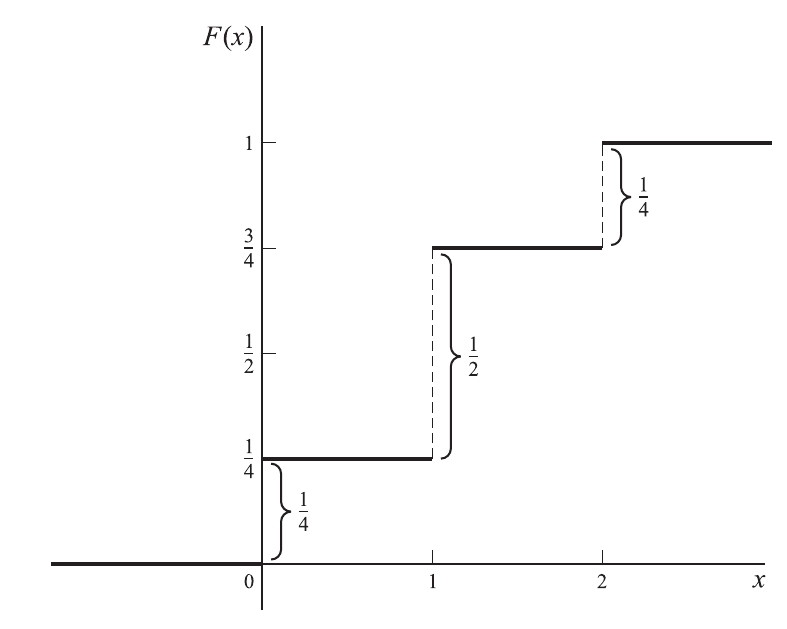
\includegraphics[height=7cm,keepaspectratio=true]{./pe/pands0201.png}
	% pands0201.png: 0x0 pixel, 300dpi, 0.00x0.00 cm, bb=
	\label{fig:0201}
\end{figure}



\begin{observacion}
	\begin{itemize}
		\item Los saltos en la función de distribución están determinados por el valor de la función de probabilidad. 
		\item Este tipo de funciones se conoce como \emph{función escalonada}.  Debe observarse que son \emph{continuas por la derecha.}
		\item La función de distribución es \emph{monótonamente creciente.}
	\end{itemize}
	
\end{observacion}



La función de probabilidad se puede obtener a partir de la función de distribución con la siguiente fórmula
\begin{align}
	\label{2.6}
	f(x)=F(x)-\lim_{u \to x^{-}}F(u).
\end{align}



\begin{ejemplo}
	\label{sol:2.3}
	\begin{enumerate}
		\item Encuentre la función de distribución $F(x)$ para la variable aleatoria del problema resuelto \ref{sol:2.1};
		\item grafique esta función de distribución.
	\end{enumerate}
	
\end{ejemplo}



\begin{figure}
	\centering
	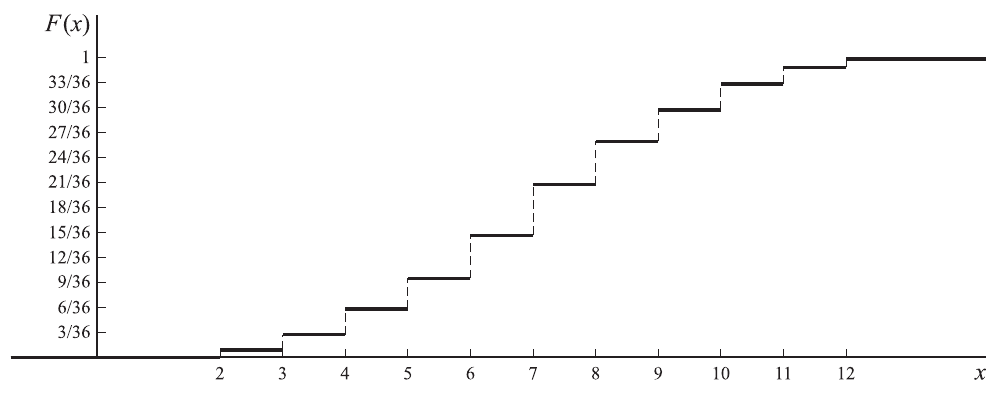
\includegraphics[width=10cm,keepaspectratio=true]{./pe/pands0206.png}
	% pands0206.png: 0x0 pixel, 300dpi, 0.00x0.00 cm, bb=
\end{figure}




\begin{ejemplo}
	\label{sol:2.4}
	\begin{enumerate}
		\item Encuentre la función de distribución $F(x)$ para la variable aleatoria del problema resuelto \ref{sol:2.2};
		\item grafique esta función de distribución.
	\end{enumerate}
	
\end{ejemplo}



\begin{figure}
	\centering
	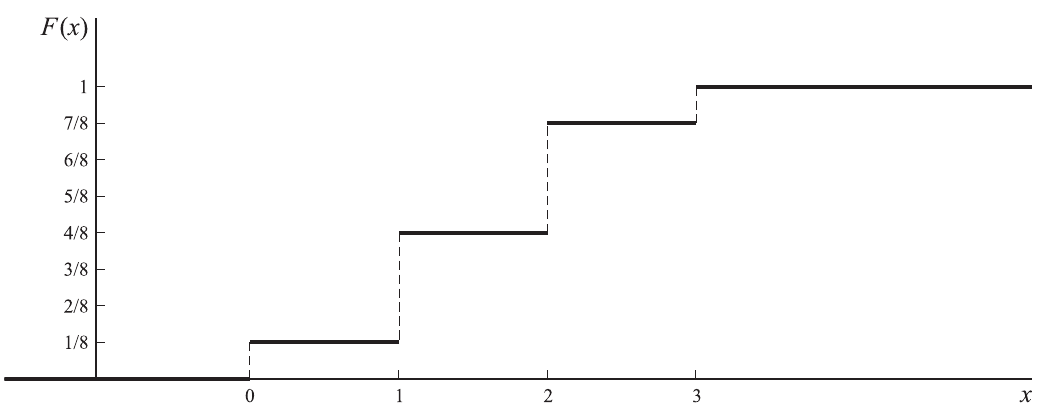
\includegraphics[width=10cm,keepaspectratio=true]{./pe/pands0207.png}
	% pands0206.png: 0x0 pixel, 300dpi, 0.00x0.00 cm, bb=
\end{figure}


\section{Variable Aleatorias Continuas}

	Una variable aleatoria no discreta $X$ se llama \emph{absolutamente continua} (o simplemente \emph{continua}) si su función de distribución puede ser representada como
	\begin{align}
		 \label{2.7}
		 F(x)=P(X \leq x)=\int_{-\infty}^{x} f(u)du, \; -\infty < x <\infty.
	\end{align}


	La función $f$ usualmente se llama \emph{densidad de probabilidad} y debe satisfacer las siguientes propiedades:
	\begin{enumerate}
		\item $f(x)\geq 0 $
		\item $\displaystyle \int_{-\infty}^{\infty}f(x)dx=1.$
	\end{enumerate}




	La probabilidad de que $X$ se encuentre entre dos valores $a$ y $b$ está dada por
	\begin{align}
		\label{2.8}
		P(a < x <b)=\int_{a}^{b}f(x)dx.
	\end{align}



	\begin{align}
		\label{exmp:2.4}
		P(X=a)=0.
	\end{align}


Por tanto, en \eqref{2.8} podemos reemplazar cualquier signo $<$ por $\leq.$


	\begin{ejemplo}
		\label{exmp:2.5}
		\begin{enumerate}
			\item Encuentre la constante $c$ tal que la función
			\begin{align}
				f(x)=
				\begin{cases}
					cx^{2} & 0 < x < 3 \\
					0 & \texttt{en otro caso}
				\end{cases}
			\end{align}
			sea una función de probabilidad. 
			\item Calcule $P(1 < X < 2).$
		\end{enumerate}

	\end{ejemplo}



	\begin{ejemplo}
	  \label{exmp:2.6}
	  Encuentre la distribución de probabilidad para la variable aleatoria del ejemplo
	  \ref{exmp:2.5} y utilícela para calcular $P(1 < x \leq 2).$
	\end{ejemplo}



	La probabilidad de que $X$ se encuentre entre $x$ y $x+\Del x$ esta dada por
	\begin{align}
		\label{2.9}
		P(x \leq X \leq x+\Del x)= \int_{x}^{x+\Del x}f(u)du,
	\end{align} 
	de manera que si $\Del x \approx 0,$ tendremos que
	\begin{align}
		\label{2.10}
		P(x \leq X \leq x+\Del x)\approx f(x) \Del x.
	\end{align}



	También podemos deducir de \eqref{2.7}, al diferenciar de ambos lados, que
	\begin{align}
		\label{2.11}
		\dfrac{dF(x)}{dx} = f(x)
	\end{align}
en todos aquellos puntos en que $f(x)$ sea continua.  Es decir, la derivada de la función de distribución es la función de densidad.


	\begin{observacion}
		Existen variables aleatorias que no son discretas ni continuas.  Por ejemplo
		\begin{align}
			F(x)=
			\begin{cases}
				0 & x <1 \\
				\frac{x}{2} & 1 \leq x < 2 \\
				1 & x \leq 2.
			\end{cases}
		\end{align}

	\end{observacion}



 \begin{ejemplo}
  \label{sol:2.5} Una variable aleatoria $X$ tiene función de densidad
  \begin{align}
   f(x)=\dfrac{c}{x^{2}+1}, \; -\infty < x <\infty.
  \end{align}

  \begin{enumerate}
   \item Encuentre el valor de $c$; 
   \item encuentre la probabilidad de que
   \begin{align}
    \dfrac{1}{3}< X^{2} <1.
   \end{align}

  \end{enumerate}

 \end{ejemplo}



 \begin{ejemplo}
  \label{sol:2.6}
  Encuentre la función de distribución correspondiente a la función de densidad del problema resuelto \ref{sol:2.5}
 \end{ejemplo}



 \begin{ejemplo}
  \label{sol:2.7}
  La función de distribución para una variable aleatoria $X$ es
  \begin{align}
   F(x)=
   \begin{cases}
    1-e^{-2x} & x\geq 0 \\
    0 & x <0
   \end{cases}
  \end{align}

  Encuentre
  \begin{enumerate}
   \item la función de densidad;
   \item la probabilidad de que $X>2$;
   \item la probabilidad que $-3 < X \leq 4.$
  \end{enumerate}


 \end{ejemplo}



\subsection{Interpretación gráfica}


	La distribución $F(x)=P(X\leq x)$ es monótonamente creciente de $0$ a $1...$
	\begin{figure}
	\centering
	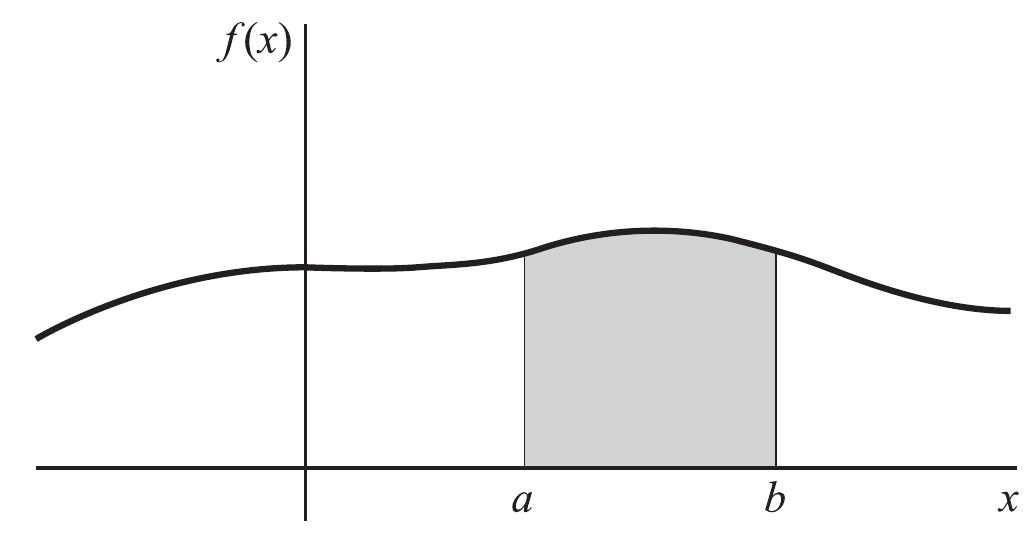
\includegraphics[height=5cm,keepaspectratio=true]{./pe/pands0202.png}
	% pands0202.png: 0x0 pixel, 300dpi, 0.00x0.00 cm, bb=
\end{figure}




  ...y el área bajo dicha curva es igual a $1.$
  \begin{figure}
	\centering
	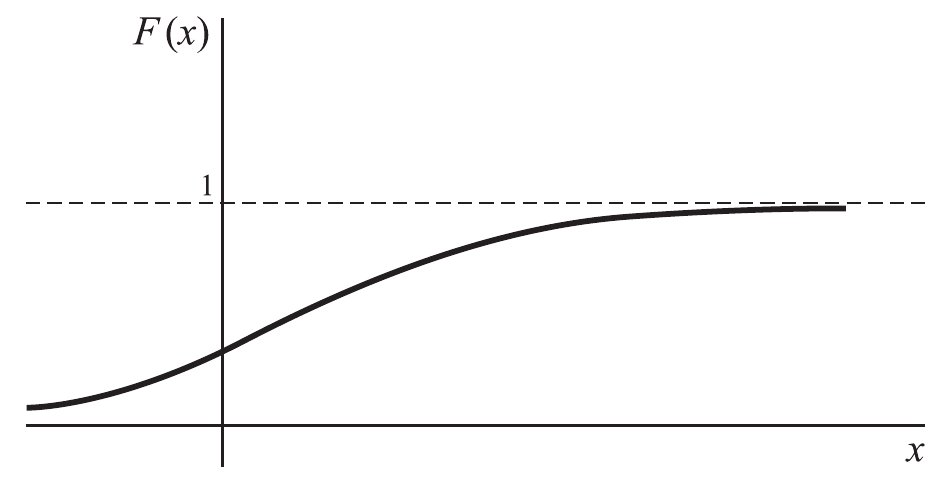
\includegraphics[height=5cm,keepaspectratio=true]{./pe/pands0203.png}
	% pands0203.png: 0x0 pixel, 300dpi, 0.00x0.00 cm, bb=
\end{figure}




\subsection{Distribución conjunta de probabilidad}


	Las ideas anteriores se generalizan fácilmente a dos o más variables.


{Caso discreto}
	Si $X$ y $Y$ son ambas variables aleatorias discretas, definimos la \emph{función de probabilidad conjunta} de $X$ y $Y$ por
	\begin{align}
	\label{2.13}
		P(X=x, Y=y)=f(x,y)
	\end{align}
 donde
\begin{enumerate}
	\item $f(x,y)\leq 0;$
	\item $\sum_{k}\sum_{y}f(x,y)=1.$
\end{enumerate}




	Supongamos que $X$ sólo toma uno de los $m$ valores $x_{1},...,x_{m},$ mientras que $Y$ tomas sólo toma uno de los $n$ valores $y_{1},...,y_{n}.$

	Entonces la probabilidad del evento $X=x_{j}, Y=y_{k}$ está dada por
	\begin{align}
	\label{2.14}
		P(X=x_{j}, Y=y_{k})=f(x_{j},y_{k})
	\end{align}



	Una función de probabilidad conjunta para $X$ y $Y$ puede ser representada por una \emph{tabla de probabilidad conjunta} como la siguiente:
	\begin{figure}
	\centering
	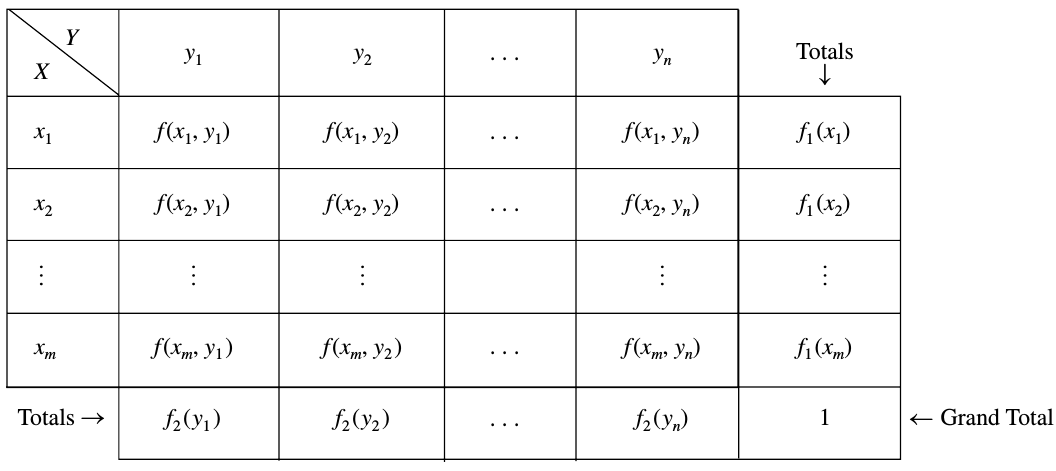
\includegraphics[height=5cm,keepaspectratio=true]{./pe/tab0203.png}
	% tab0203.png: 0x0 pixel, 300dpi, 0.00x0.00 cm, bb=
	\label{tab:0203}
\end{figure}



	La probabilidad de $X=x_{j}$ se obtiene de la siguiente manera
	\begin{align}
	\label{2.15}
		P(X=x_{j})=f_{X}(x_{j})=\sum_{k=1}^{n}f(x_{j},y_{k}).
	\end{align}



	De manera similar, la probabilidad de $Y=y_{k}$ se obtiene de la siguiente manera
	\begin{align}
	\label{2.16}
		P(Y=y_{k})=f_{Y}(y_{k})=\sum_{j=1}^{m}f(x_{j},y_{k}).
	\end{align}


 
 	Nos referiremos a $f_{X}(x)$ y $f_{Y}(y)$ como \emph{funciones de probabilidad marginal} de $X$ y $Y$ respectivamente.
 

	Observe que
	\begin{align}
	\label{2.17}
		\sum_{j=1}^{m}f_{X}(x_{j})=1,
		\sum_{k=1}^{n}f_{Y}(y_{k})=1,
	\end{align}
	lo cual se puede reescribir como
	\begin{align}
		\label{2.18}
		\sum_{j=1}^{m}\sum_{k=1}^{n}f(x_{j},y_{k})=1.
	\end{align}



	La \emph{función de distribución conjunta } está definida por
	\begin{align}
	\label{2.19}
		F(x,y)=P(X\leq x, Y\leq y)
		=\sum_{u\leq x}\sum_{v\leq y}f(u,v)
	\end{align}



{Caso continuo}
	El caso en el que ambas variables son continuas es obtenido de manera análoga reemplazando las sumas por integrales.


	La \emph{función de probabilidad conjunta} (o de manera más común \emph{función de densidad conjunta}) de $X$y $Y$ está definida por
	\begin{enumerate}
		\item $f(x,y)\geq 0;$
		\item $\displaystyle \int_{-\infty}^{\infty}\int_{-\infty}^{\infty}
		f(x,y) dxdy=1.$
	\end{enumerate}



	Gráficamente $z=f(x,y)$ representa una \emph{superficie de probabilidad}
\begin{figure}
	\centering
	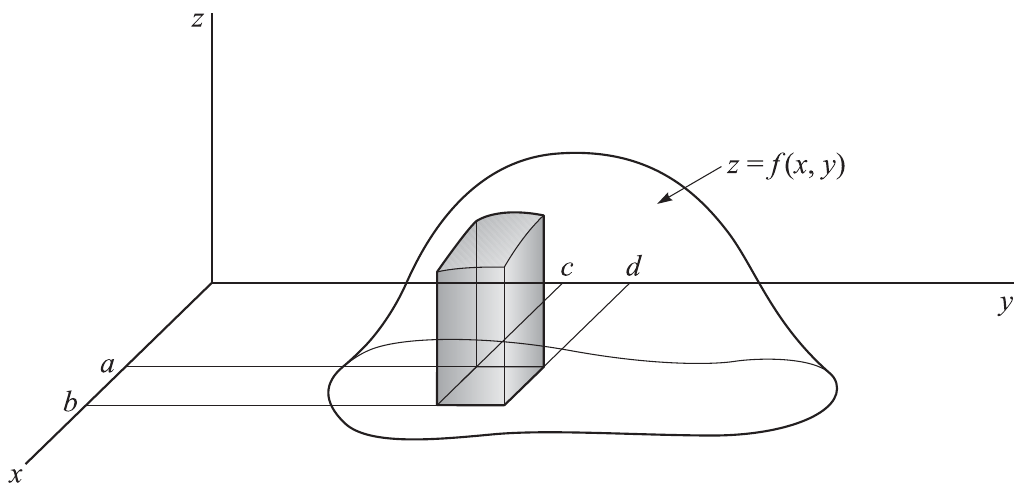
\includegraphics[height=3cm,keepaspectratio=true]{./pe/pands0204.png}
	% pands0204.png: 0x0 pixel, 300dpi, 0.00x0.00 cm, bb=
	\label{fig:2.4}
\end{figure}
tal que el volumen bajo la superficie es igual a $1.$


	\begin{align}
		\label{2.20}
		P(a<X<b,c<Y<d)=\int_{a}^{b}\int_{c}^{d}f(x,y)dydx.
	\end{align}



	A cada evento $A$ corresponde una región $\mathcal{R}_{A}$ del plano $xy$ tal que
	\begin{align}
	  \label{2.21}
		P(A)=\iint_{\mathcal{R}_{A}}f(x,y)dxdy.
	\end{align}



	La \emph{función de distribución conjunta} de $X$ y $Y$ en este caso está definida por
	\begin{align}
		\label{2.22}
	F(x,y)=P(X\leq x, Y\leq y)=
	\int_{-\infty}^{x} \int_{-\infty}^{y} f(u,v)dvdu.
	\end{align}



	Se sigue que
	\begin{align}
	 \dfrac{\partial^{2}F}{\partial x \partial y}=
	 f(x,y)  \label{2.23} \\
	  	 P(X\leq x)=F_{X}(x)=\int_{-\infty}^{x}\int_{-\infty}^{\infty} f(u,v)dvdu \label{2.24} \\
	 	 P(Y\leq y)=F_{Y}(y)=\int_{-\infty}^{\infty}\int_{-\infty}^{y} f(u,v)dvdu \label{2.25}
	\end{align}



 Diremos que $F_{X}(x),F_{Y}(y)$ son las \emph{funciones de distribución marginal,} o simplemente \emph{funciones distribuciones,} de $X$ y $Y$, respectivamente.


 Las derivadas de \eqref{2.24} y \eqref{2.25} con respecto a $x$ y $y$ son llamadas \emph{funciones de densidad marginal}, o simplemente las \emph{funciones de densidad,} de $X$ y $Y$ están dados por
 \begin{align}
 \label{2.26}
 \displaystyle
  f_{X}(x)=\int_{-\infty}^{\infty}f(x,v)dv, \;
  f_{Y}(x)=\int_{-\infty}^{\infty}f(u,y)du.
 \end{align}



\subsection{Variables Aleatorias Independientes}

 Supongamos que $X$ y $Y$ son variables aleatorias discretas.  Si los eventos $X=x$ y $Y=y$ son eventos independientes para todo $x,y,$  entonces diremos que $X,Y$ son v.a's independientes.


 En tal caso,
 \begin{align}
  \label{2.27}
  P(X=x,Y=y)=P(X=x)P(Y=y),
 \end{align}
o de manera equivalente
\begin{align}
 f(x,y)=f_{X}(x)f_{Y}(y).
\end{align}



 De manera inversa, si para todo $x,y$ la función de probabilidad conjunta $f(x,y)$ pueden ser expresada como el producto de funciones de probabilidad marginal $f_{X}(x)f_{Y}(y),$ entonces $X,Y$ son independientes.
 

 Si no pueden expresarse de dicha manera, entonces $X,Y$ son dependientes.


 Si $X,Y$ son v.a's continuas, diremos que son \emph{independientes} si los eventos $X\leq x$ y $Y\leq y$ son independientes para todo $x,y.$

 En tal caso, escribiremos
 \begin{align}
  \label{2.29}
  P(X\leq x, Y \leq y)=P(X\leq x)P(Y\leq y)
 \end{align} 
 o de manera equivalente
 \begin{align}
  F(x,y)=F_{X}(x)F_{Y}(y)
 \end{align}
 donde $F_{X}(x)$ y $F_{Y}(y)$ son las funciones de distribución marginal de $X,Y$ respectivamente.



 De manera inversa, si para todo $x,y$ la función de probabilidad conjunta $f(x,y)$ pueden ser expresada como el producto de funciones de probabilidad marginal $F_{X}(x)F_{Y}(y),$ entonces $X,Y$ son independientes.
 

 Si no pueden expresarse de dicha manera, entonces $X,Y$ son dependientes.


 Para v.a's independientes continuas, también es cierto que la función de densidad conjunta $f(x,y)$ es el producto de funciones $f_{X}(x)f_{Y}(y)$ y estas son las funciones de densidad marginal de $X,Y$ respectivamente.



 \begin{ejemplo}
  \label{sol:2.8}
  La función de probabilidad conjunta de dos variables discretas $X,Y$ está dada por
  \begin{align}
   f(x,y)=
   \begin{cases}
    c(2x+y) & 0\leq x \leq 2, \; 0 \leq y \leq 3 \\
    0 & \texttt{en otro caso}.
   \end{cases}
  \end{align}
  \begin{enumerate}
   \item Encuentre el valor de la constante $c;$
   \item encuentre $P(X=2,Y=1);$
   \item encuentre $P(X\geq 1, Y\leq 2).$
  \end{enumerate}

 \end{ejemplo}



 \begin{figure}
 \centering
 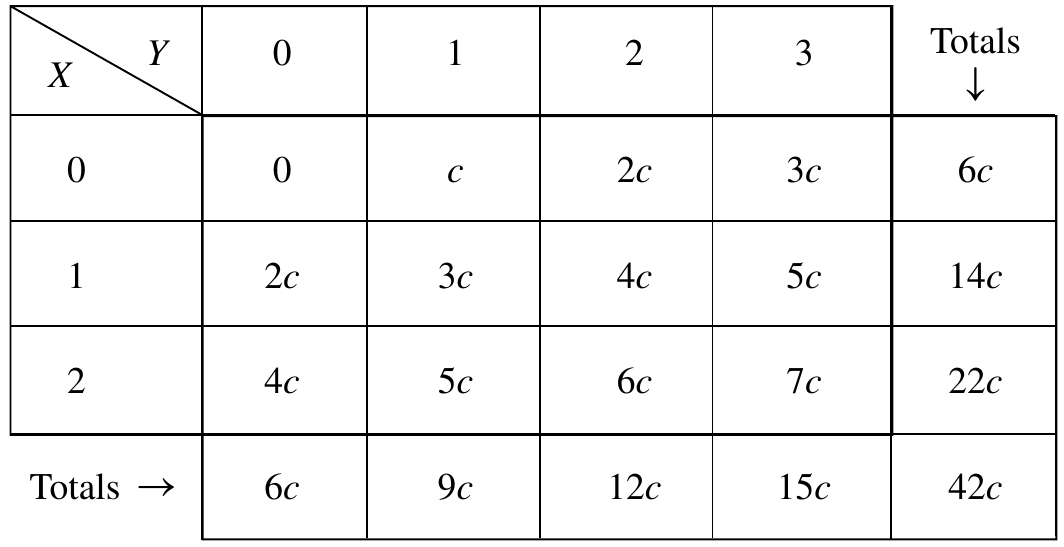
\includegraphics[width=10cm,keepaspectratio=true]{./pe/tab0206.png}
 % tab0206.png: 0x0 pixel, 300dpi, 0.00x0.00 cm, bb=
 \label{tab:2.6}
\end{figure}



 \begin{ejemplo}
  \label{sol:2.9}
  Encuentre las funciones de probabilidad marginal para $X$ y $Y$ en el problema resuelto \ref{sol:2.8}.
 \end{ejemplo}



 \begin{ejemplo}
  \label{sol:2.10}
  Muestre que las variables aleatorias del problema resuelto \ref{sol:2.8} son dependientes.
 \end{ejemplo}



 \begin{ejemplo}
  \label{sol:2.11}
  La función de densidad conjunta de dos variables aleatorias continuas $X$ y $Y$ es
  \begin{align}
   f(x,y)=
   \begin{cases}
    cxy & 0<x<4, \; 1<y<5\\
    0 & \texttt{en otro caso}.
   \end{cases}
  \end{align}

 \end{ejemplo}
\begin{enumerate}
 \item Encuentre el valor de $c$;
 \item encuentre $P(1<X<2,2<Y<3)$;
 \item encuentre $P(X\geq 3, Y\leq 2)$.
\end{enumerate}



 \begin{ejemplo}
  \label{sol:2.12}
  Encuentre las funciones de probabilidad marginal de las v.a's $X,Y$ del problema resuelto \ref{sol:2.11}.
 \end{ejemplo}



 \begin{ejemplo}
  \label{sol:2.13}
  Encuentre la función de distribución conjunta para las v.a's del problema resuelto \ref{sol:2.11}.
 \end{ejemplo}



 \begin{center}
 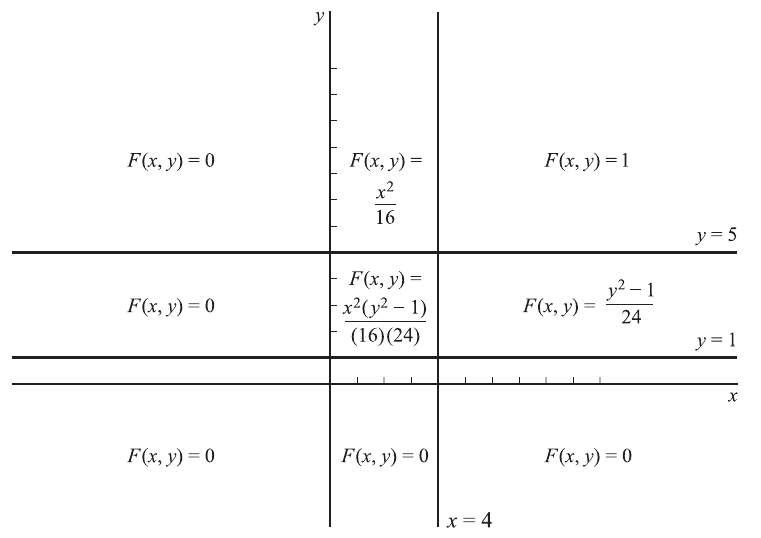
\includegraphics[width=10cm,keepaspectratio=true]{./pe/pands0209.png}
 % pands0209.png: 0x0 pixel, 300dpi, 0.00x0.00 cm, bb=
\end{center}




 \begin{ejemplo}
  \label{sol:2.14}
  En el problema resuelto \ref{sol:2.11}, encuentre $P(X+Y<3)$.
 \end{ejemplo}



 \begin{center}
 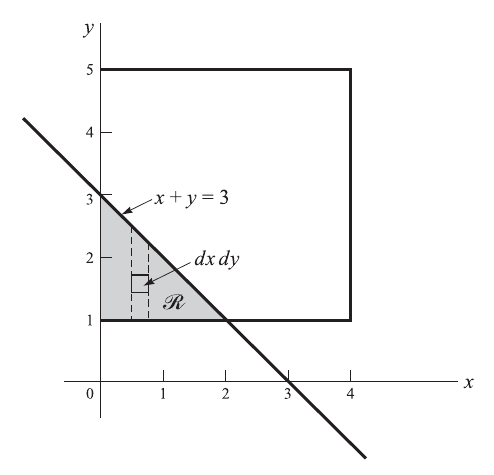
\includegraphics[height=8cm,keepaspectratio=true]{./pe/pands0210.png}
 % pands0210.png: 0x0 pixel, 300dpi, 0.00x0.00 cm, bb=
\end{center}



\subsection{Distribución Condicional}

 Nosotros ya sabemos que si $P(A)>0,$
 \begin{align}
  \label{2.41}
  P(B|A)=\dfrac{P(A\cap B)}{P(A)}.
 \end{align}



 Si $X,Y$ son v.a's discretas y tenemos los eventos $A=\set{X=x}, \; B=\set{Y=y},$ entonces \eqref{2.41} se convierte
 \begin{align}
  \label{2.42}
  P(Y=y|X=x)=
  \begin{cases}
   \dfrac{f(x,y)}{f_{X}(x)} & 0 < f_{X}(x)  \\
   0 & \texttt{en otro caso}
  \end{cases}
 \end{align}
 $f(x,y)=P(X=x,Y=y)$ es la función de probabilidad conjunta, mientras que $f_{X}(x)$ es la función de probabilidad marginal para $X.$


 Definimos la \emph{función de probabilidad condicional de $Y$ dado $X$} como
 \begin{align}
  \label{2.43}
  f(y|x)=
  \begin{cases}
   \dfrac{f(x,y)}{f_{X}(x)} & 0 < f_{X}(x)  \\
   0 & \texttt{en otro caso}
  \end{cases}
 \end{align}



 De manera similar, definimos la \emph{función de probabilidad condicional de $X$ dado $Y$} como
 \begin{align}
  \label{2.44}
  f(x|y)=
  \begin{cases}
   \dfrac{f(x,y)}{f_{Y}(y)} & 0 < f_{Y}(y)  \\
   0 & \texttt{en otro caso}
  \end{cases}
 \end{align}


 Estas ideas son fácilmente extensibles al caso donde $X,Y$ son v.a's continuas.


 Por ejemplo, la \emph{función de densidad condicional de $Y$ dado $X$} es
 \begin{align}
  \label{2.45}
  f(y|x)=
    \begin{cases}
   \dfrac{f(x,y)}{f_{X}(x)} & 0 < f_{X}(x)  \\
   0 & \texttt{en otro caso}
  \end{cases}
 \end{align}
 donde $f(x,y)$ es la función de densidad conjunta de $X$ y $Y$ y $f_{X}(x)$ es la función de densidad marginal de $X.$


 Usando \eqref{2.45} podemos por ejemplo encontrar que la probabilidad que $Y$  se encuentre entre $c$ y $d$ dado que $X=x$ es
 \begin{align}
  \label{2.46}P(c<Y<d|X=x)=
  \int_{c}^{d}f(y|x)dy.
 \end{align}




 \begin{ejemplo}
  \label{sol:2.27}
  Para la distribución del problema resuelto \ref{sol:2.8}, encuentre
  \begin{enumerate}
   \item $f(y|2)$; y  
   \item $P(Y=1|X=2)$
  \end{enumerate}

 \end{ejemplo}



\begin{ejemplo}
 \label{sol:2.28}
  Si $X$ y $Y$ tienen función de densidad conjunta
 \begin{align}
  f(x,y)=
  \begin{cases}
   \frac{3}{4}+xy & 0<x<1, \; 0<y<1 \\
   0 & \texttt{en otro caso},
  \end{cases}
 \end{align}
encuentre
\begin{enumerate}
 \item $f(y|x)$; 
 \item $P(Y>\frac{1}{2}| X = \frac{1}{2} )$.
\end{enumerate}

\end{ejemplo}



 \begin{ejemplo}
  \label{sol:2.29}
  La función de densidad conjunta de las variables aleatorias $X$ y $Y$ está dada por
  \begin{align}
   f(x,y)=
   \begin{cases}
    8xy & 0\leq x \leq 1, 0\leq y \leq x \\
    0 & \texttt{en otro caso}.
   \end{cases}
  \end{align}
Encuentre
\begin{enumerate}
 \item la densidad marginal de $X$; 
 \item la densidad marginal de $Y$; 
 \item la densidad condicional de $X$; 
 \item la densidad condicional de $Y$.
\end{enumerate}

 \end{ejemplo}



 \begin{center}
 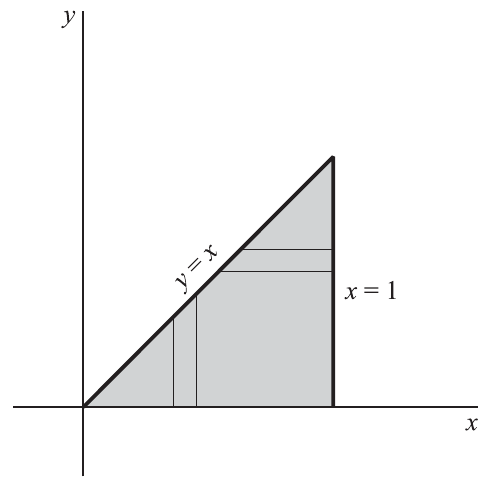
\includegraphics[height=7cm,keepaspectratio=true]{./pe/pands0217.png}
 % pands0217.png: 0x0 pixel, 300dpi, 0.00x0.00 cm, bb=
\end{center}



 \begin{ejemplo}
  \label{sol:2.30}
  Determine si las v.a's del problema resuelto \ref{sol:2.29} son independientes.
 \end{ejemplo}



\section{Esperanza Matemática}

\subsection{Definición de Esperanza Matemática}


  Para una variable aleatoria discreta $X$ que toma valores $x_{1},...,x_{n},$ la \emph{esperanza matemática} se define como
  \begin{align}
   \label{eq:3.1}
   E(X)=\sum _{j=1}^{n} x_{j}P(X=x_{j})=:\sum xP(X=x),
  \end{align}

o de manera equivalente
  \begin{align}
   \label{eq:3.2}
   E(X)=\sum _{j=1}^{n} x_{j}f(x_{j})=:\sum xf(x),
  \end{align}
  donde $f(x)=P(X=x).$



 Como un caso especial, cuando $f(x)\equiv \frac{1}{n},$ obtenemos la \emph{media aritmética:}
 \begin{align}
  \label{eq:3.3}
  E(X)=\dfrac{\sum_{i=1}^{n}x_{i}}{n}.
 \end{align}


{}
\begin{ejemplo}
 Sea $X$ el número que se obtiene al lanzar un dado.  Entonces, cada cara $x$ tiene la misma probabilidad
 \begin{align}
 f(x) = \frac{1}{6}
\end{align} de caer.


Por tanto,
$E(X)= (1)\left( \frac{1}{6} \right)+...+(6)\left( \frac{1}{6} \right) = \dfrac{1+...+6}{6} = 3.5$
\end{ejemplo}



{Caso Discreto Numerable}
 En el caso en que $X$ tome un cantidad (infinita) numerable de valores $x_{1},x_{2},...,$ definimos
 \begin{align}
  E(X)=\sum_{i=1}^{\infty}x_{i}f(x_{i}),
 \end{align}
siempre y cuando dicha \emph{serie} converja.


% {}
% La serie anterior debe entenderse como el límite
% $\lim_{n\to \infty} \sum_{i=1}^{n} x_{i}f(x_{i}).$
%
%
% 

{Caso Continuo}
 Para una variable aleatoria continua $X$ que tenga función de densidad $f(x),$ la esperanza de $X$ se define como
 \begin{align}
  \label{eq:3.4}
  E(X)=\int_{-\infty}^{\infty}xf(x)dx
 \end{align}
siempre y cuando dicha \emph{integral} converja.


 La esperanza de $X$ es llamada a menudo \emph{media} de $X$ y es denotada por $\mu_{x},$ o simplemente $\mu,$ cuando la variable aleatoria subyacente se sobreentiende.


 La media o esperanza de $X$ da un único valor que representa el promedio de los valores de $X,$ y por esta razón decimos que es una \emph{medida de tendencia central.}



 \begin{ejemplo}
  \label{exmp:3.1}
  Supongamos que un juego se juega con un dado único que se suponen justos. En este juego, un jugador gana \$20 si un sale un $2$; \$40 con un $4$; \$30 con un $6$; y no gana ni pierde con cualquier otra cara. Encuentre la suma esperada de dinero que ganaría.
 \end{ejemplo}





 \begin{align}
 \mu &= \$ 20 \left( \frac{1}{6} \right) + \$40 \left( \frac{1}{6} \right) + \$60\left( \frac{1}{6} \right) \\
   &= \dfrac{\$20 + \$40 + \$60 + 3\times\$ 0}{6} \\
   &= \$ 15
\end{align}




 \begin{ejemplo}
  \label{exmp:3.2}
  La función de densidad de una variable aleatoria $X$ está dada por
  \begin{align}
   f(x)=
   \begin{cases}
    \frac{1}{2}x & 0<x<2 \\
    0 & \texttt{en otro caso}
   \end{cases}
  \end{align}
Encuentre el valor esperado de $X.$
 \end{ejemplo}



{}
\begin{align}
 \mu &= E(X)\\ & = \int_{-\infty}^{\infty} xf(x) dx \\
  &= \int_{0}^{2} x\left( \dfrac{1}{2}x \right) dx\\
  &= \evat{\frac{1}{6} \, x^{3}}{0}{2}\\
  &= \frac{1}{6}(2)^{3}-\frac{1}{6}(0)^{3} \\
  &= \frac{4}{3}
\end{align}


\subsection{Funciones de Variables Aleatorias}

 Sea $X$ una variable aleatoria discreta con función de probabilidad $f(x).$ Entonces $Y=g(X)$ es una variable aleatoria discreta con función de probabilidad
 \begin{align}
  h(y)=P(g(X)=y)=\sum_{\set{x|g(x)=y}}g(x)f(x)
 \end{align}



 Entonces, en el caso discreto.
 \begin{align}
 \label{eq:3.5}
  E\left( g(X) \right)=
  \sum_{x}g(x)f(x)
 \end{align}

 De manera similar, en el caso continuo
 \begin{align}
  \label{eq:3.6}
  E\left( g(X) \right)=\int_{-\infty}^{\infty}
  g(x)f(x)dx.
 \end{align}




 \begin{ejemplo}
  \label{exmp:3.3}
  Si $X$ es la variable aleatoria del ejemplo \ref{exmp:3.2}, encuentre $E\left( 3X^{2}-2X \right).$
 \end{ejemplo}


{}
En este caso, $g(x)=3x^2-2x.$



Recordemos que
  \begin{align}
   f(x)=
   \begin{cases}
    \frac{1}{2}x & 0<x<2 \\
    0 & \texttt{en otro caso}
   \end{cases}
  \end{align}



\begin{align}
 E(3X^2-2X) &= E(g(X)) \\
  &= \displaystyle \int_{-\infty}^{\infty} \left( 3x^2-2x \right)f(x)dx\\
  &= \displaystyle \int_{0}^{2}\left( 3x^2-2x \right)\left( \dfrac{1}{2}x \right)dx \\
  &= \displaystyle \int_{0}^{2} \frac{3}{2} \, x^{3} - x^{2} dx
 \\  &= \displaystyle \evat{\frac{3}{8} \, x^{4} - \frac{1}{3} \, x^{3}
}{0}{2}
\\  &= \displaystyle
\frac{10}{3}
\end{align}


\subsection{Algunos temas sobre esperanza matemática}
{Linealidad}
 \begin{teorema}
  \label{thm:3.1}
  Si $c,d$ son constantes y $X,Y$ son variables aleatorias, entonces
  \begin{align}
   \label{linealidad}
   E\left( cX+dY \right)=
   cE\left( X \right)+dE\left( Y \right)
  \end{align}

 \end{teorema}


{Esperanza e independencia}
 \begin{teorema}
  \label{thm:3.3} Si $X,Y$ son \emph{variables aleatorias independientes}, entonces
  \begin{align}
   \label{eq:3.10}
   E\left( XY \right)=E(X)E(Y)
  \end{align}

 \end{teorema}



\subsection{Varianza y Desviación Estándar}

 Ya vimos que la espereza matemática de una variable aleatoria $X$ es una medida de tendencia central y que generaliza a la \emph{media aritmética $\mu$.}
 

\begin{observacion}
 Por esta razón, de aquí en adelante definiremos
 \begin{align}
  \mu=\mu_{X}=E(X).
 \end{align}

\end{observacion}

 


 Otra cantidad de gran importancia es la \emph{varianza} que se define como
 \begin{align}
  \label{eq:3.11}
  \s_{X}^{2}=\Var(X)=E\left( \left( X-\mu_{X} \right)^{2} \right)
 \end{align}



 La \emph{desviación estándar} se definirá como
 \begin{align}
  \label{eq:3.12}
  \s_{X} = \sqrt{\Var{X}}
 \end{align}



 \begin{observacion}
  Si la variable aleatoria $X$ se sobreentiende del contexto, omitiremos el subíndice correspondiente, es decir,
  \begin{align}
   \mu=\mu_{X}, \; \s=\s_{X}, \; \s^{2}=\s_{X}^{2}.
  \end{align}

 \end{observacion}



 Si $X$ es una variable aleatoria discreta, la varianza está dada por
 \begin{align}
  \label{eq:3.13}
  \s^{2}=E\left( \left( X-\mu \right)^{2} \right)=\sum\left( x-\mu \right)^{2}f(x),
 \end{align}
 siempre y cuando esta suma converja.


En el caso de que todas las probabilidades sean iguales y la variable aleatoria $X$ sea finita tenemos
\begin{align}
\label{eq:3.14}
 \s^{2}=\dfrac{\left( x_{1}-\mu \right)^{2}+...+\left( x_{n}-\mu \right)^{2} }{n}
\end{align}



{}
\begin{ejemplo}
 Como vimos anteriormente, si $X$ es la cara obtenida al lanzar un dado, entonces $\mu_{X}=3.5$.


La varianza de $X$ es
\begin{align}
 \s^{2}
 &= \displaystyle \dfrac{(1-3.5)^2+...+(6-3.5)^2}{6}
 \\  &= \displaystyle \frac{17.5}{6}
 \\  &\approx \displaystyle 2.916
\end{align}
\end{ejemplo}




 Si $X$ es una variable aleatoria continua con función de densidad $f(x),$ entonces la varianza está dada por
 \begin{align}
  \label{eq:3.15}
  \s^{2}=E\left( (X-\mu)^{2} \right)=
  \int_{-\infty}^{\infty}\left( x-\mu \right)^{2}f(x)dx
 \end{align}
siempre y cuando la integral converja.


 Tanto la varianza como la desviación estándar es una \emph{medida de dispersión.}
 \begin{figure}
 \centering
 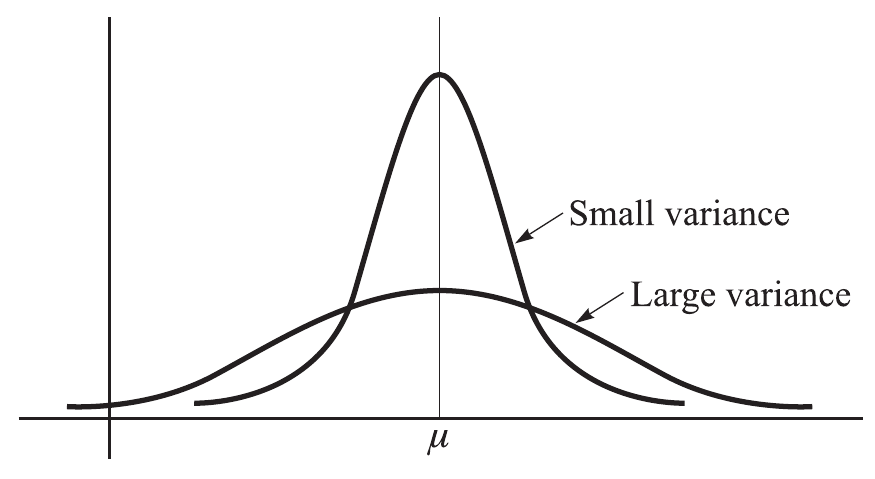
\includegraphics[height=5cm,keepaspectratio=true]{./pe/pands0301.png}
 % pands0301.png: 0x0 pixel, 300dpi, 0.00x0.00 cm, bb=
 \label{fig:0301}
\end{figure}



 \begin{ejemplo} %falta escribir esto en la libreta
  \label{exmp:3.4}
  Encuentre la varianza y la desviación estándar de la variable aleatoria del ejemplo \ref{exmp:3.2}.
 \end{ejemplo}


{}
Recordemos que esta variable aleatoria $X$ tiene densidad de probabilidad
  \begin{align}
   f(x)=
   \begin{cases}
    \frac{1}{2}x & 0<x<2 \\
    0 & \texttt{en otro caso}
   \end{cases}
  \end{align}

{}
\begin{align}
 \sigma^2 = Var(X) &= \displaystyle \int_{0}^{2}(x-\frac{4}{3})^2f(x) dx
 \\  &= \displaystyle \int_{0}^{2} \frac{1}{2} \, {\left(x - \frac{4}{3}\right)}^{2} x dx
 \\  &= \displaystyle
 \evat{\frac{1}{8} \, x^{4} - \frac{4}{9} \, x^{3} + \frac{4}{9} \, x^{2}}{0}{2}
 \\  &= \displaystyle \frac{2}{9}
\\  &\approx \displaystyle 0.\bar{2}
\end{align}

{Algunos teoremas sobre Varianza}
\begin{align}
 \label{eq:3.16}
 \s^{2}=E\left( X^{2} \right)-\mu^{2} \\ 
 \label{eq:3.17}
 \Var\left( cX \right)=c^{2}\Var\left( X \right)\\ 
 \label{thm:3.6}
 \s^{2}=\min_{a}\set{E\left( \left( X-a \right)^{2} \right)}
\end{align}

Si $X,Y$ son independientes
\begin{align}
 \label{eq:3.18}
 \Var(X\pm Y)=\Var(X)+\Var(Y)
\end{align}


{Variables Aleatorias Estandarizadas}
 Sea $X$ una variable aleatoria con media $\mu$ y desviación estándar $\s>0.$ Diremos que la \emph{variable aleatoria estandarizada} asociada está dada por
 \begin{align}
  \label{eq:3.20}
  X^{*}=\dfrac{X-\mu}{\s}.
 \end{align}


\begin{align}
 \label{eq:3.21}
 E\left( X^{*} \right)=0, \; \Var(X^{*})=1.
\end{align}


\subsection{Covarianza y correlación}

Los resultados dados anteriormente para una variable aleatoria pueden extenderse a dos variables.


{}

\begin{equation}
 \label{eq:3.43}
 \begin{split}
  \mu_{X}=E(X)=\int_{-\infty}^{\infty}\int_{-\infty}^{\infty} xf(x,y)dxdy\\ 
  \mu_{Y}=E(Y)=\int_{-\infty}^{\infty}\int_{-\infty}^{\infty}
  yf(x,y)dxdy
 \end{split}
\end{equation}





\begin{equation}
 \label{eq:3.44}
 \begin{split}
  \s^{2}_{X}=E\left( (X-\mu_{X})^{2} \right)=\int_{-\infty}^{\infty}\int_{-\infty}^{\infty} (x-\mu_{X})^2f(x,y)dxdy\\ 
  \s^{2}_{Y}=E\left( (Y-\mu_{Y})^{2} \right)=\int_{-\infty}^{\infty}\int_{-\infty}^{\infty} (y-\mu_{Y})^2f(x,y)dxdy
 \end{split}
\end{equation}


{Covarianza}
 \begin{align}
 \label{eq:3.45}
  \s_{XY}=\cov(X,Y)=E\left( (X-\mu_{X})(Y-\mu_{Y}) \right)
 \end{align}



 \begin{align}
  \label{eq:3.46}
  \s_{XY}=\int_{-\infty}^{\infty}
  \int_{-\infty}^{\infty}
  (x-\mu_{X})(y-\mu_{Y})f(x,y)dxdy
 \end{align}


{Caso Discreto}

 \begin{equation}
  \begin{split}
   \mu_{X}=\sum_{x}\sum_{y}xf(x,y) \\
  \mu_{Y}=\sum_{x}\sum_{y}yf(x,y)
  \end{split}
 \end{equation}



 \begin{align}
  \label{eq:3.48}
  \s_{XY}=\sum_{x}\sum_{y}(x-\mu_{X})(y-\mu_{Y})f(x,y)
 \end{align}



 \begin{align}
  \label{eq:3.50}
  \s_{XY}=E(XY)-E(X)E(Y)=E(XY)-\mu_{X}\mu_{Y}
 \end{align}


 Si $X,Y$ son independientes, entonces
 \begin{align}
  \label{eq:3.50}
  \s_{XY}=\cov(X,Y)=0
 \end{align}



 \begin{align}
  \label{eq:3.51}
  \Var(X\pm Y)=\Var(X)\pm2\cov(X,Y)+\Var(Y).
 \end{align}




 De manera equivalente,
 \begin{align}
  \label{eq:3.52}
  \s_{X\pm Y}^{2}=\s_{X}^{2} \pm 2\s_{XY} +\s_{Y}^{2}
 \end{align}


{Coeficiente de correlación de Pearson}
 \begin{align}
  \label{eq:3.54}
  \rho = \dfrac{\s_{XY}}{\s_{X}\s_{Y}}
 \end{align}



 \begin{teorema}
  \begin{align}
   \label{eq:3.53}
   \abs{\s_{XY}}\leq \s_{X}\s_{Y}
  \end{align}


 \begin{align}
  \abs{\rho}\leq 1.
 \end{align}
 \end{teorema}


{Propiedades de la correlación}

\begin{enumerate}
\item $-1 \leq \rho \leq 1$ 
 \item $\rho \approx 0$: \emph{Correlación débil}, prácticamente no existe una correlación lineal. 
 \item $\abs{\rho} \approx 1$:\emph{ Correlación fuerte}, la correlación está dada prácticamente por una función afín $y=mx+b$. 
 \item $\rho > 0$: \emph{Correlación positiva}, en la medida que una crece, la otra también crece. 
 \item $\rho < 0$: \emph{Correlación negativa}, en la medida que una crece, la otra decrece.
\end{enumerate}



 \begin{ejemplo}
  \label{sol:3.25}
  \emph{Sean $X,Y$ variables aleatorias discretas} con densidad de probabilidad conjunta
  \begin{align}f(x,y)=
   \begin{cases}
    \dfrac{2x+y}{42} & 0\leq x \leq 2,\; 0\leq y \leq 3 \\
    0 & \texttt{en otro caso}.
   \end{cases}
  \end{align}
 \end{ejemplo}
 

Encuentre los siguientes estadísticos:
\begin{multicols}{3}
 \begin{enumerate}
 \item $\mu_X = E(X)$ %
 \item $\mu_Y = E(Y)$ %
 \item $ E(XY)$ %
 \item $E(X^2)$ %
 \item $E(Y^2)$ %
 \item $\s^2_X = \Var(X)$ %
 \item $\s_{Y}$
 \item $\s^2_Y = \Var(Y)$ %
 \item $\s_{Y}$
 \item $\s_{XY} =\cov(X,Y)$ %
 \item $\rho$
\end{enumerate}
\end{multicols}






 \begin{ejemplo}
  \label{sol:3.26}
  \emph{Sean $X,Y$ variables aleatorias continuas} con densidad de probabilidad conjunta
  \begin{align}f(x,y)=
   \begin{cases}
    \frac{1}{210}(2x+y) & 2 < x < 6,\; 0<y<5 \\
    0 & \texttt{en otro caso}.
   \end{cases}
  \end{align}
 \end{ejemplo}

 

Encuentre los siguientes estadísticos:
\begin{multicols}{3}
 \begin{enumerate}
 \item $\mu_X = E(X)$ %
 \item $\mu_Y = E(Y)$ %
 \item $ E(XY)$ %
 \item $E(X^2)$ %
 \item $E(Y^2)$ %
 \item $\s^2_X = \Var(X)$ %
 \item $\s_{Y}$
 \item $\s^2_Y = \Var(Y)$ %
 \item $\s_{Y}$
 \item $\s_{XY} =\cov(X,Y)$ %
 \item $\rho$
\end{enumerate}
\end{multicols}





\section{Distribuciones especiales}


\subsection{La Distribución Binomial}


 Si $p$ es la probabilidad de que en un solo ensayo ocurra un evento (llamada la probabilidad de éxito) y $q = 1 - p$ es la
probabilidad de que este evento no ocurra en un solo ensayo (llamada probabilidad de fracaso), entonces la probabilidad de que el evento ocurra exactamente $x$ veces en $N$ ensayos (es decir, que ocurran $x$ éxitos y $N - x$ fracasos) está
dada por
\begin{align}
 \label{eq:7.1}
 f(x)=P(X=x)=\comb{N}{x}p^{x}q^{N-x}
\end{align}
donde $x=0,1,...,N.$


 \begin{ejemplo}
  \label{exmp:7.1}
  La probabilidad de obtener exactamente dos caras en seis lanzamientos de una moneda es
  \begin{align}
   \comb{6}{2}\left( \dfrac{1}{2} \right)^{2}\left( \dfrac{1}{2} \right)^{6-2}=\dfrac{15}{64}
  \end{align}
empleando \eqref{eq:7.1} con $N=6, x=2, p=q=\frac{1}{2}.$
 \end{ejemplo}



\begin{ejemplo}
 \label{exmp:7.2}
 Calcule la probabilidad de obtener al menos 4 caras en 6 lanzamientos de una moneda.
\end{ejemplo}



 En lo subsecuente, daremos por hecho que hemos importado los siguientes paquetes:
 \begin{itemize}
  \item \texttt{scipy.stats}
  \item \texttt{numpy} como \texttt{np}
 \end{itemize}


[fragile, allowframebreaks]{statsBinom.py}
\begin{verbatim}
from scipy import stats
import numpy as np
import matplotlib.pyplot as plt

#Consideremos 6 experimentos con p de éxito 1/2
p=0.5
N=6
binDist = stats.binom(N,p)
#probabilidad de obtener dos éxitos
print binDist.pmf(2)
##0.234375
#probabilidad de obtener al menos 4 éxitos
print sum(binDist.pmf(np.arange(4,6+1)))
##0.34375
 \end{verbatim}


 \begin{ejemplo}
  \label{exmp:7.3}
  Desarrolle $\left( p+q \right)^{4}.$
 \end{ejemplo}


[fragile, allowframebreaks]{coefBinom.py}
\begin{verbatim}

from scipy import stats
import numpy as np

#coeficientes de (p+q)^4
p=.5
N=4
binomDist = stats.binom(N,p)
binDistExmp = binomDist.pmf(np.arange(5))
print binDistExmp*2**N
##[ 1.  4.  6.  4.  1.]
\end{verbatim}


{Propiedades de la distribución binomial} Supongamos que realizamos $N$ experimentos con probabilidad éxito $p$ y de fracaso $q=1-p.$
\begin{align}
 \label{binom:mean}
 \mu = Np \\
 \label{binom:var}
 \s^{2}=Npq
\end{align}


[fragile,allowframebreaks]{histBinom.py}
 \begin{verbatim}
import numpy as np
import matplotlib.pyplot as plt

#Ejemplo de distribución binomial
N,p=100, 0.5
s = np.random.binomial(N,p,1000)

miHist = np.histogram(s, bins = np.arange(100+1))
print miHist[0]
print miHist[1]
print np.mean(s)
print N*p
print np.var(s)
print N*p*(1-p)

plt.hist(s, bins = np.arange(100+1))
plt.show()
 \end{verbatim}




 \begin{figure}
 \centering
 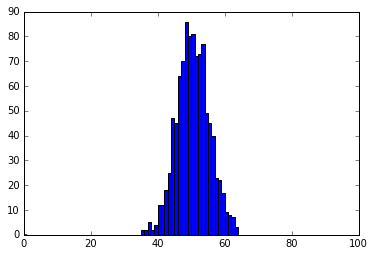
\includegraphics[height=7cm,keepaspectratio=true]{./pe/distBin01.png}
 % distBin01.png: 0x0 pixel, 300dpi, 0.00x0.00 cm, bb=
 \label{distBin01}
\end{figure}


\subsection{Distribución Normal}

 Una de las distribuciones de probabilidad continua más importantes es la \emph{distribución normal}, también llamada \emph{distribución gaussiana,} que se define mediante la función de densidad
 \begin{align}
  \label{eq:7.3_}
  f_{a,b}(x)=\dfrac{1}{\sqrt{2\pi}}e^{-\frac{1}{2}\frac{(x-a)^{2}}{b^{2}}}
 \end{align}
donde $a,b$ son parámetros específicos para cada v.a. $X.$

{Propiedades de la distribución normal}
 Si la v.a. $X$ tiene la función de densidad dada por \eqref{eq:7.3_}, con parámetros $a,b$ entonces
 \begin{align}
  a = \mu_{X}\\
  b = \s_{X}
 \end{align}



 Si una variable aleatoria normal $X$ tiene función de densidad
  \begin{align}
  \label{eq:7.3_}
  f(x)=\dfrac{1}{\sqrt{2\pi}}e^{-\frac{1}{2}\frac{(x-\mu)^{2}}{\s^{2}}},
 \end{align}
 escribiremos $X\sim N(\mu, \s^{2}).$


{Variable aleatoria normalizada}
 \begin{align}
  \label{van}
  Z = \dfrac{X-\mu}{\s}\\
  \mu_{Z}=0 \\
  \s_{Z}=1
 \end{align}


{Forma Estándar}
 \begin{align}
  \label{eq:7.4}
  f(z)=\dfrac{1}{\sqrt{2\pi}}e^{-\frac{1}{2}z^{2}}
 \end{align}


En este caso, diremos que $Z$ está \emph{normalmente distribuida.}


[fragile, allowframebreaks]{distribucionNormal.py}
 \begin{verbatim}
import scipy.integrate as integrate
import numpy as np
import matplotlib.pyplot as plt
from matplotlib.patches import Polygon

def fn(x,m=0,s=1):
    return np.exp(-(x-m)**2/(2*s**2))/(s*np.sqrt(2*np.pi))
x1 = np.arange(-4,4,0.1)
plt.plot(x1, fn(x1))
plt.show()

for s in np.arange(1,4+1):
    result = integrate.quad(lambda x:fn(x),-s,s)
    print result

for s in np.arange(1,4+1):
    result = integrate.quad(lambda x:fn(x),-s,s)

    a, b = -s, s  # integral limits
    x = np.arange(-4,4,0.01)
    y = fn(x)

    fig, ax = plt.subplots()
    plt.plot(x, y, 'r', linewidth=2)
    plt.ylim(ymin=0)

    # Make the shaded region
    ix = np.linspace(a, b)
    iy = fn(ix)
    verts = [(a, 0)] + list(zip(ix, iy)) + [(b, 0)]
    poly = Polygon(verts, facecolor='0.9', edgecolor='0.5')
    ax.add_patch(poly)

    ax.set_xticks((a, b))
    ax.set_xticklabels(('$-\sigma$', '$\sigma$'))
    ax.set_yticks([])

    plt.show()
    print result
 \end{verbatim}


[fragile]
 \begin{figure}
 \centering
 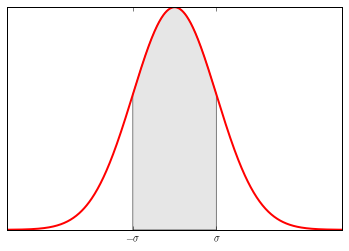
\includegraphics[height=5cm,keepaspectratio=true]{./pe/norm1.png}
 % norm1.png: 0x0 pixel, 300dpi, 0.00x0.00 cm, bb=
 \label{fig:norm1}
\end{figure}
\begin{verbatim}
 #(0.682689492137086, 7.579375928402476e-15)
\end{verbatim}


[fragile]
 \begin{figure}
 \centering
 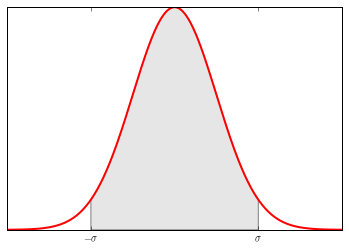
\includegraphics[height=5cm,keepaspectratio=true]{./pe/norm2.png}
 % norm1.png: 0x0 pixel, 300dpi, 0.00x0.00 cm, bb=
 \label{fig:norm2}
\end{figure}
\begin{verbatim}
 #(0.9544997361036417, 1.8403548653972355e-11)
\end{verbatim}


[fragile]
 \begin{figure}
 \centering
 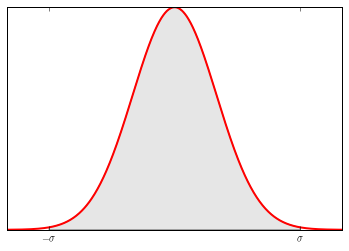
\includegraphics[height=5cm,keepaspectratio=true]{./pe/norm3.png}
 % norm1.png: 0x0 pixel, 300dpi, 0.00x0.00 cm, bb=
 \label{fig:norm3}
\end{figure}
\begin{verbatim}
 #(0.9973002039367399, 1.1072256503105314e-14)
\end{verbatim}


[fragile]
 \begin{figure}
 \centering
 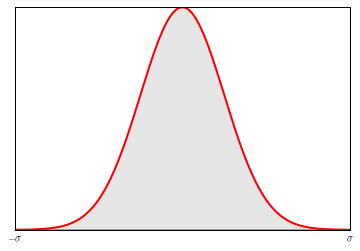
\includegraphics[height=5cm,keepaspectratio=true]{./pe/norm4.png}
 % norm1.png: 0x0 pixel, 300dpi, 0.00x0.00 cm, bb=
 \label{fig:norm4}
\end{figure}
\begin{verbatim}
 #(0.9999366575163339, 4.838904125482879e-12)
\end{verbatim}


[fragile, allowframebreaks]{normalCDF.py}
 \begin{verbatim}
from scipy import stats
import numpy as np
import matplotlib.pyplot as plt

mu = 3.5
sigma = 0.76
nd = stats.norm(mu, sigma)

x = np.arange(mu - 4*sigma,mu + 4*sigma,0.01)
y = nd.cdf(x)

fig, ax = plt.subplots()
plt.plot(x, y, 'r', linewidth=2)
plt.ylim(ymin=0)

for k in range(1,5):
    print nd.cdf(mu+k*sigma)-nd.cdf(mu-k*sigma)

#0.682689492137
#0.954499736104
#0.997300203937
#0.999936657516
 \end{verbatim}
\begin{center}
 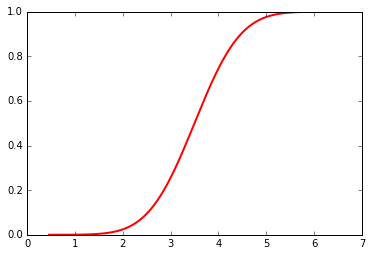
\includegraphics[height=5cm,keepaspectratio=true]{./pe/normCDF.png}
 % normCDF.png: 0x0 pixel, 300dpi, 0.00x0.00 cm, bb=
\end{center}



\subsection{Relación entre las distribuciones binomial y normal}

 Si $N\sim \infty, p,q>>0,$ y $X$ es un distribución binomial con parámetros $N,p$ entonces
 \begin{align}
  \dfrac{X-Np}{\sqrt{Npq}} \sim N(0,1).
 \end{align}



 \begin{ejemplo}
  \label{exmp:7.5}
  Consideremos el experimento de lanzar 16 veces una moneda. Repitamos 1,000,000 dicho experimento. Compruebe que dicho experimento se puede modelar por una variable aleatoria con distribución $N(\mu=8,\sigma^{2}=4)$
 \end{ejemplo}


[fragile, allowframebreaks]{relBinomNormal.py}
 \begin{verbatim}
import numpy as np
import matplotlib.pyplot as plt

def fn(x,m=0,s=1):
    C = 1/(s*np.sqrt(2*np.pi))
    return C*np.exp(-(x-m)**2/(2*s**2))

N,p=30, 0.5
R = 1000000
q=1-p
mB = N*p
sB = np.sqrt(N*p*q)
X = np.random.binomial(N,p,R)
myBins = np.arange(-0.5,N+0.5,1)
plt.hist(X, bins = myBins)
x = np.arange(mB-4*sB,mB+4*sB+0.1,0.1)
y = R*fn(x, m=mB, s=sB)
plt.plot(x,y,lw=2)
plt.ylim(ymin=0)
plt.show()
 \end{verbatim}
\begin{center}
 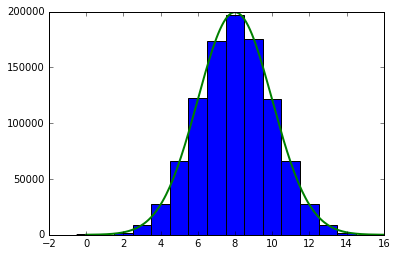
\includegraphics[height=5cm]{./pe/relBinNorm.png}
 % relBinNorm.png: 0x0 pixel, 300dpi, 0.00x0.00 cm, bb=
\end{center}



\subsection{La Distribución de Poisson}
{Distribución de Poisson} Diremos que una variable aleatoria \emph{discreta} $X$ tiene distribución de Poisson si su función de probabilidad está dada por:
 \begin{align}
  \label{eq:7.5}
  f(n)=\dfrac{\lam^{n}e^{-\lam}}{n!}, \; n=0,1,2,...
 \end{align}


En este caso, $\mu_{X}=\s^{2}=\lam.$


\begin{quote}
 En teoría de probabilidad y estadística, la distribución de Poisson es una distribución de probabilidad discreta que expresa, a partir de una frecuencia de ocurrencia media, la probabilidad de que ocurra un determinado número de eventos durante cierto período de tiempo. Concretamente, se especializa en la probabilidad de ocurrencia de sucesos con probabilidades muy pequeñas, o sucesos raros.
\end{quote}

\href{https://es.wikipedia.org/wiki/Distribuci\%C3\%B3n_de_Poisson}{Wikipedia: Distribución de Poisson}


 \begin{ejemplo}
  \label{exmp:7.6}
  El número de personas por día que llegan a una sala de urgencias tiene una distribución de Poisson con media 5. Hallar la probabilidad de que cuando mucho lleguen tres por día y la probabilidad de que por lo menos lleguen 8 personas por día.
 \end{ejemplo}




[fragile, allowframebreaks]{distPoisson.py}
 \begin{verbatim}
from scipy import stats
import numpy as np
import matplotlib.pyplot as plt

def f(x, mu=1):
    return stats.poisson.pmf(x, mu)

def F(x, mu=1):
    return stats.poisson.cdf(x, mu)

x1 = np.arange(0,100+1)
plt.plot(x1, f(x1, mu=5), 'bo')
plt.show()

s = np.random.poisson(5,365)
M = np.max(s)
myBins = np.arange(0,M+1)
plt.hist(s, bins = myBins)
plt.show()

print F(3, mu=5)
print 1 - F(7, mu=5)

for k in range(12+1):
    print k, F(k, 5)
"""
0 0.00673794699909
1 0.0404276819945
2 0.124652019483
3 0.265025915297
4 0.440493285065
5 0.615960654833
6 0.762183462973
7 0.86662832593
8 0.931906365278
9 0.968171942694
10 0.986304731402
11 0.994546908087
12 0.997981148373
"""
 \end{verbatim}



 \begin{figure}
 \centering
 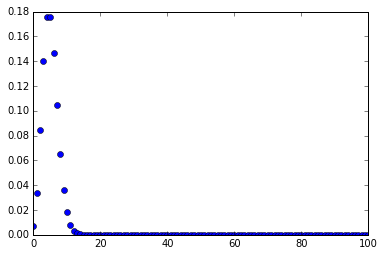
\includegraphics[height=7cm,keepaspectratio=true]{./pe/distPoisson0.png}
 % distPoisson0.png: 0x0 pixel, 300dpi, 0.00x0.00 cm, bb=
 \caption{Distribución de Poisson}
\end{figure}




\begin{figure}
 \centering
 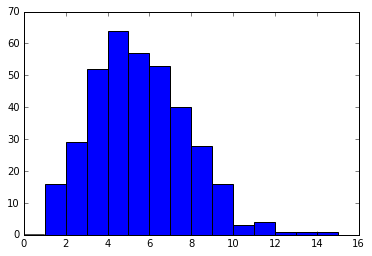
\includegraphics[height=7cm,keepaspectratio=true]{./pe/distPoisson1.png}
 % distPoisson1.png: 0x0 pixel, 300dpi, 0.00x0.00 cm, bb=
 \caption{Histograma de pacientes en sala de urgencias durante un año con media $\lam=5$}
 \label{fig:distPoisson1}
\end{figure}



\subsection{Relación entre las Distribuciones Binomiales y de Poisson}

 Si en la función de probabilidad binomial, $N$ es muy grande pero $p \approx 0,$ esto modela un \emph{evento raro}.  En la práctica esto significa $N>>50, Np<<5.$ 

 En este caso, la distribución Binomial con parámetros $N,p$ se aproxima a una Poisson con parámetro $\lam = Np.$

[fragile, allowframebreaks]{relBinomPoisson.py}
 \begin{verbatim}
from scipy import stats
import numpy as np
import matplotlib.pyplot as plt
import matplotlib as mpl

mpl.style.use("ggplot")

fig, ax = plt.subplots(1, 1)

def fP(x, mu=1):
    return stats.poisson.pmf(x, mu)

def fB(x, N=30, p=0.5):
    return stats.binom(N,p).pmf(x)

N_=50
p_=5./N_
mu_ = N_*p_
x1 = np.arange(0,20+1)
ax.plot(x1, fP(x1, mu=mu_), 'bo', label="Poisson")
ax.plot(x1, fB(x1, N=N_, p=p_), 'ro', label="Binomial")
legend = ax.legend(loc='upper center', shadow=True)
plt.show()

 \end{verbatim}



 \begin{figure}
 \centering
 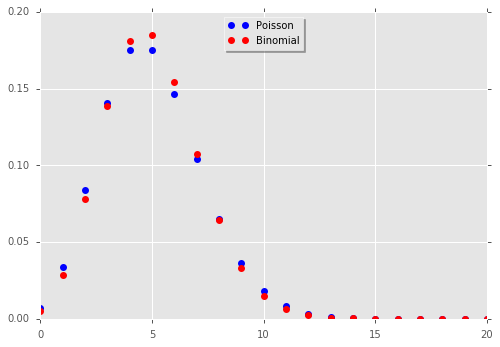
\includegraphics[height=7cm]{./pe/binVsPoi.png}
 % binVsPoi.png: 0x0 pixel, 300dpi, 0.00x0.00 cm, bb=
 \caption{Comparación entre distribuciones Binomial y Poisson para eventos raros.}
\end{figure}



\subsection{Distribución multinomial}

 Si los eventos $E_{1},...,E_{k}$ pueden ocurrir con probabilidades $p_{1},...,p_{k}$ respectivamente, entonces la probabilidad de que ocurran $X_{1},...,x_{k}$ veces respectivamente esta dado por la \emph{distribución multinomial}
 \begin{align}
  \label{eq:7.6}
  f\left( x_{1},...,x_{2} \right)=
  \dfrac{x_{1}+...+x_{k}}{x_{1}!...x_{k}!}p_{1}^{x_{1}}\cdots p_{k}^{x_{k}}.
 \end{align}



 \begin{ejemplo}
  \label{exmp:7.7}
Si un dado se lanza 12 veces, encontrar la probabilidad de obtener cada uno de los números $1,2,3,4,5,6$ exactamente dos veces.
 \end{ejemplo}



\subsection{Problemas Resueltos}
{Percentil}
 Diremos que $x=P_{q}$ es el percentil $q, \; 0\leq q \leq 100$ de la distribución $F(x)$ si $F(P_{q})=q\%.$  En el caso de que $q$ sea un valor realizable de $F(x),$ podemos \emph{``despejar''}
 \begin{align}
  P_{q}=F^{-1}\left( \dfrac{q}{100} \right).
 \end{align}
 A tal función se le llama \emph{distribución inversa.}


{Cuartiles}
 En la literatura se definen conceptos similares. Por ejemplo, el primer \emph{cuartil} corresponde al percentil $25;$ el segundo cuartil al percentil $50;$ y así sucesivamente.

{Combinaciones}
 \begin{ejemplo}
  \label{sol:7.1}
  Encuentre
  \begin{enumerate}
   \item $5!$
   \item $\comb{8}{3}$
  \end{enumerate}
  utilizando \texttt{Python.}
 \end{ejemplo}


[fragile, allowframebreaks]{combinaciones.py}
 \begin{verbatim}
import math
import scipy.special

print math.factorial(5)
print scipy.special.binom(8,3)
 \end{verbatim}




{Distribución Binomial}
 \begin{ejemplo}
  \label{sol:7.2}
  Supóngase que $15\%$ de la población es zurda. Encontrar la probabilidad de que en un grupo de 50 individuos haya:
  \begin{enumerate}
   \item cuando mucho 10 zurdos; 
   \item por lo menos 5 zurdos; 
   \item entre 3 y 6 zurdos; 
   \item exactamente 5 zurdos.
  \end{enumerate}

 \end{ejemplo}


[fragile, allowframebreaks]{solvedBinom.py}
 \begin{verbatim}
from scipy import stats

#7.2 N=50, p=15%
def f(x):
    return stats.binom(50,.15).pmf(x)
def F(x):
    return stats.binom(50,.15).cdf(x)
#(a) P(X<=10)
print sum([f(x) for x in range(0,10+1)])
##0.8800826828
print F(10)
##0.8800826828
#(b) P(X>=5)
print 1-sum([f(x) for x in range(0,4+1)])
##0.887894791945
print 1-F(4)
##0.887894791945
#(c) P(3<=X<=6)
print sum([f(x) for x in range(3,6+1)])
##0.3471108697
print F(6)-F(2)
##0.3471108697
#(d) P(X=5)
print f(5)
##0.3471108697
 \end{verbatim}



{Distribución Normal}
 \begin{ejemplo}
  \label{sol:7.14}
  En un examen final de matemáticas, la media fue 72 y la desviación estándar fue 15. Determinar las puntuaciones estándar de los estudiantes que obtuvieron:
  \begin{enumerate}
   \item $60$;
   \item $93$;
   \item $72$.
  \end{enumerate}

 \end{ejemplo}



 \begin{ejemplo}
  \label{sol:7.15}
  Con los datos del problema \ref{sol:7.14}, encontrar las calificaciones que corresponden a las siguientes puntuaciones estándar:
  \begin{enumerate}
   \item $-1$;
   \item $1.6$.
  \end{enumerate}

 \end{ejemplo}



 \begin{ejemplo}
  \label{sol:7.16}
  Supóngase que la cantidad de juegos en que participan los beisbolistas de la liga mayor durante su carrera se distribuye normalmente con media de $1500$ juegos y desviación estándar $350$ juegos. Emplear \texttt{Python} para responder las siguientes preguntas:
  \begin{enumerate}
   \item ¿Qué porcentaje participa en menos de 750 juegos?;
   \item ¿qué porcentaje participa en más de 2000 juegos?;
   \item encontrar el \emph{percentil} $90$ de la cantidad de juegos en los que participan en su carrera.
  \end{enumerate}

 \end{ejemplo}


[fragile, allowframebreaks]{solvedNorm.py}
 \begin{verbatim}
from scipy import stats

mu = 1500
sigma = 350
nd = stats.norm(mu, sigma)

def F(x):
    return nd.cdf(x)

#a
print F(750)
##0.3471108697

#b
print 1-F(2000)
##0.0765637255098

def inverseF(x):
    return nd.ppf(x)
#c
print inverseF(.90)
##1948.54304794
 \end{verbatim}


{Eventos raros}
\begin{ejemplo}
\label{sol:7.28}
  Si la probabilidad de que un individuo tenga una reacción adversa por la inyección de determinado suero es $0.001,$ determinar la probabilidad de que de 2000 individuos:
 \begin{enumerate}
  \item exactamente 3;
  \item más de 2
 \end{enumerate}
sufran una reacción adversa.
\end{ejemplo}


[fragile, allowframebreaks]{eventosRaros.py}
 \begin{verbatim}
from scipy import stats
#7.28
#a
N = 2000
p = 0.001
print stats.binom(N,p).pmf(3)
##0.180537328032
print stats.poisson(N*p).pmf(3)
##0.180447044315
#(b)
print 1-stats.binom(N,p).cdf(2)
##0.32332356124
print 1-stats.poisson(N*p).cdf(2)
##0.323323583817
 \end{verbatim}



%%%%%%%%%%%%%%%%%%%%%%%%%%%%%%
\chapter{Estadística Inferencial}
\section{Conceptos más importantes}

% []
% \tableofcontents
\begin{enumerate}
\item Pruebas de hipótesis.
\item $p-$valores.
\item Distribución normal.
\item Correlación.
\end{enumerate}


\subsection{Muestreo aleatorio y teorema del límite central}
Entender el concepto de \emph{muestreo aleatorio} a través de ejemplos e ilustrar las aplicaciones del \emph{teorema del límite central}. 

  Estos dos conceptos son la columna vertebral de las pruebas de hipótesis.


\subsection{Pruebas de hipótesis}
Entender el significado de los términos tales como \emph{hipótesis nula}, \emph{hipótesis alternativa}, \emph{intervalos de confianza}, \emph{$p-$valores}, \emph{nivel de significación}, etc.
%   Desarrollaremos una guía de la implementación de pruebas de hipótesis, seguidas por un ejemplo.

\subsection{Pruebas $\chi-$cuadrada}
Calcularemos el estadístico $\chi$-cuadrada y describiremos el uso de pruebas $\chi$-cuadrada con un par de ejemplos.

 \subsection{Correlación}
  Entenderemos el significado y la significación de la correlación entre dos variables, de los coeficientes de correlación y calcularemos y visualizaremos la correlación entre variables de una base de datos.
 

\section{Muestreo aleatorio y teorema del límite central}

\subsection{Ejemplo}
Supongamos que tratamos de encontrar la edad promedio en una ciudad, digamos Oaxaca. Una manera de hacerlo sería por \emph{fuerza bruta}, es decir, recolectando esta información persona por persona. Pero este método sería muy costoso en términos de infraestructura y tiempo.


En estadística, este es un problemalema común, cuya solución está en el \emph{muestreo aleatorio}:  Tomemos un grupo de 1000 individuos (o 10,000 dependiendo de tu capacidad, obviamente entre más, es mejor) y calculemos la edad promedio en este grupo, a la que denotaremos por $A_{1}.$ 


Repitamos este procedimiento, digamos 100 veces, y denotaremos por $A_{1}, A_{2},...,A_{100}$ el promedio de edades obtenido en cada respectivo intento.

De acuerdo a la \emph{ley de los grandes números}, la cantidad
\begin{align}
	\bar{A}_{100}=\dfrac{A_{1}+...+A_{100}}{100}
\end{align}
es una aproximación muy cercana al promedio real de la edad de los pobladores de la ciudad.


De acuerdo al \emph{teorema del límite central}, si el número de tales muestras es suficientemente grande,
$A_{1},A_{2},...,A_{100}$ estarán distribuidos de manera normal.


\begin{observacion}
	No estamos más interesados en obtener el valor exacto de la edad promedio, si no establecer un \emph{estimador} para la misma. 
	
	En tal caso,
	tenemos que conformarnos con la definición de un \emph{rango de valores} en el que el valor real podría estar.
\end{observacion}


% 
% Dado que hemos supuesto una \emph{distribución normal} para los valores de edad media de estos
% grupos, podemos \emph{aplicar todas las propiedades} de una distribución normal para
% posibilidades de que la edad \emph{promedio} este en algún \emph{intervalo}.
% 

\section{Pruebas de hipótesis}
% 
% El concepto que acabamos de comentar en la sección anterior se utiliza para una
% técnica en estadística, llamada \emph{prueba de hipótesis}.
% 


En la prueba de hipótesis, asumimos una
premisa inicial (generalmente relacionada con el valor del estimador) denominada \emph{hipótesis nula}  y
trataremos de ver si es cierta o no aplicando.



Tenemos otra premisa llamada \emph{hipótesis alternativa}, la cuál es la negación de la hipótesis nula.


\subsection{Hipótesis nula vs. alternativa}
%  Hay una forma para decidir cuál será la hipótesis nula y cuál será la hipótesis alternativa. 
%
% La hipótesis nula es la premisa inicial o algo que
% podemos suponer que es cierto. 
%
% Por el contrario, la hipótesis alternativa es algo de lo que no estamos seguros que podría ser cierto.
% 
%
% 
Cuando alguien está haciendo una \emph{investigación} cuantitativa para calibrar el valor de un estimador,  el \emph{valor conocido} del parámetro se toma como \emph{hipótesis nula},  mientras que el \emph{nuevo valor} encontrado (de la investigación) se toma como la \emph{hipótesis alternativa}.



En nuestro caso (encontrar la edad media de nuestra ciudad), un investigador puede afirmar que la edad
\emph{menor que 35}. Esto puede servir como la \emph{hipótesis nula}.


Si una nueva agencia afirma
que es \emph{mayor que 35}, entonces se puede denominar como la \emph{hipótesis alternativa}.


\section{Estadísticos Z y t}

\begin{enumerate}
	\item Suponga que el valor del parámetro asumido en la hipótesis nula es $Ao$. 
	\item Tomemos
	una muestra aleatoria de 100 o 1000 personas o eventos del evento. 
	\item Calculemos
	la media del parámetro, por ejemplo la edad promedio de una ciudad, el tiempo medio de suministro de la pizza, la media
	ingresos, etc. 
	\item Podemos llamarlo $A$.
\end{enumerate}




El estadístico $Z$ se calcula para convertir una variable normalmente distribuida (por ejemplo, la distribución de la media poblacional de edad) a una distribución normal estándar.
%  Esto es porque los valores de problemaabilidad para una variable que sigue a la distribución normal estandarizada se puede obtener de una tabla precalculada.


El estadístico $Z$ se da por la siguiente fórmula:
\begin{align}
	\label{zStat}
	Z=\dfrac{A-A_{0}}{{\sigma}/{\sqrt{n}}}
\end{align}
donde $\s$ es la desviación estándar de la población y $n$ es el número de personas en la muestra


Ahora, debemos considerar dos casos

\paragraph{Prueba Z (distribución normal)}
El investigador conoce a desviación estándar del parámetro de su experiencia pasada.



Un buen ejemplo de esto es el caso del tiempo de entrega de una pizza.  En este caso \eqref{zStat} seguirá una distribución normal y los valores normalizados se conocerán como \emph{valores Z}.

\paragraph{Prueba t (distribución t de Student) }
En este caso, el investigador no conoce la desviación estándar de la población.



Esto puede pasar porque:
\begin{itemize}
	\item No existen tales datos en algún registro histórico;
	\item o el número de eventos o personas es demasiado pequeño para suponer una distribución normal.
\end{itemize}


En este caso, la media y la desviación estándar son desconocidas, y la expresión asume una distribución diferente a la normal llamada \emph{distribución $t$ de Student}.



El valor estandarizadas en este caso es llamado \emph{$t-$valor} y la prueba es llamada \emph{prueba-$t$}.


\paragraph{Distribución t de Student}
\begin{quote}
	La distribución de Student fue descrita en 1908 por William Sealy Gosset. Gosset trabajaba en una fábrica de cerveza, Guinness, que prohibía a sus empleados la publicación de artículos científicos debido a una difusión previa de secretos industriales. De ahí que Gosset publicase sus resultados bajo el seudónimo de Student. \footnote{
		\href{https://es.wikipedia.org/wiki/Distribuci\%C3\%B3n\_t\_de\_Student\#Historia}{Wikipedia: Distribución $t$ de Student}
	}
\end{quote}


\begin{figure}
	\centering
	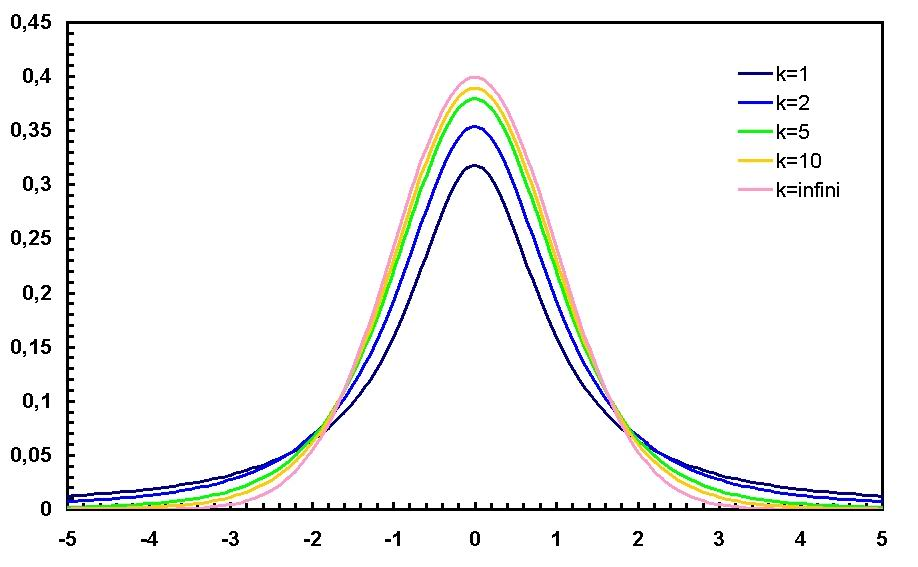
\includegraphics[height=5cm,keepaspectratio=true]{./images/Student_densite_best.jpg}
	% Student_densite_best.jpg: 0x0 pixel, 300dpi, 0.00x0.00 cm, bb=
	\caption{De The original uploader was Thorin de Wikipedia en francés - Transferido desde fr.wikipedia a Commons., CC BY-SA 1.0, https://commons.wikimedia.org/w/index.php?curid=1878902}
	\label{fig:tPDF}
\end{figure}




\begin{figure}
	\centering
	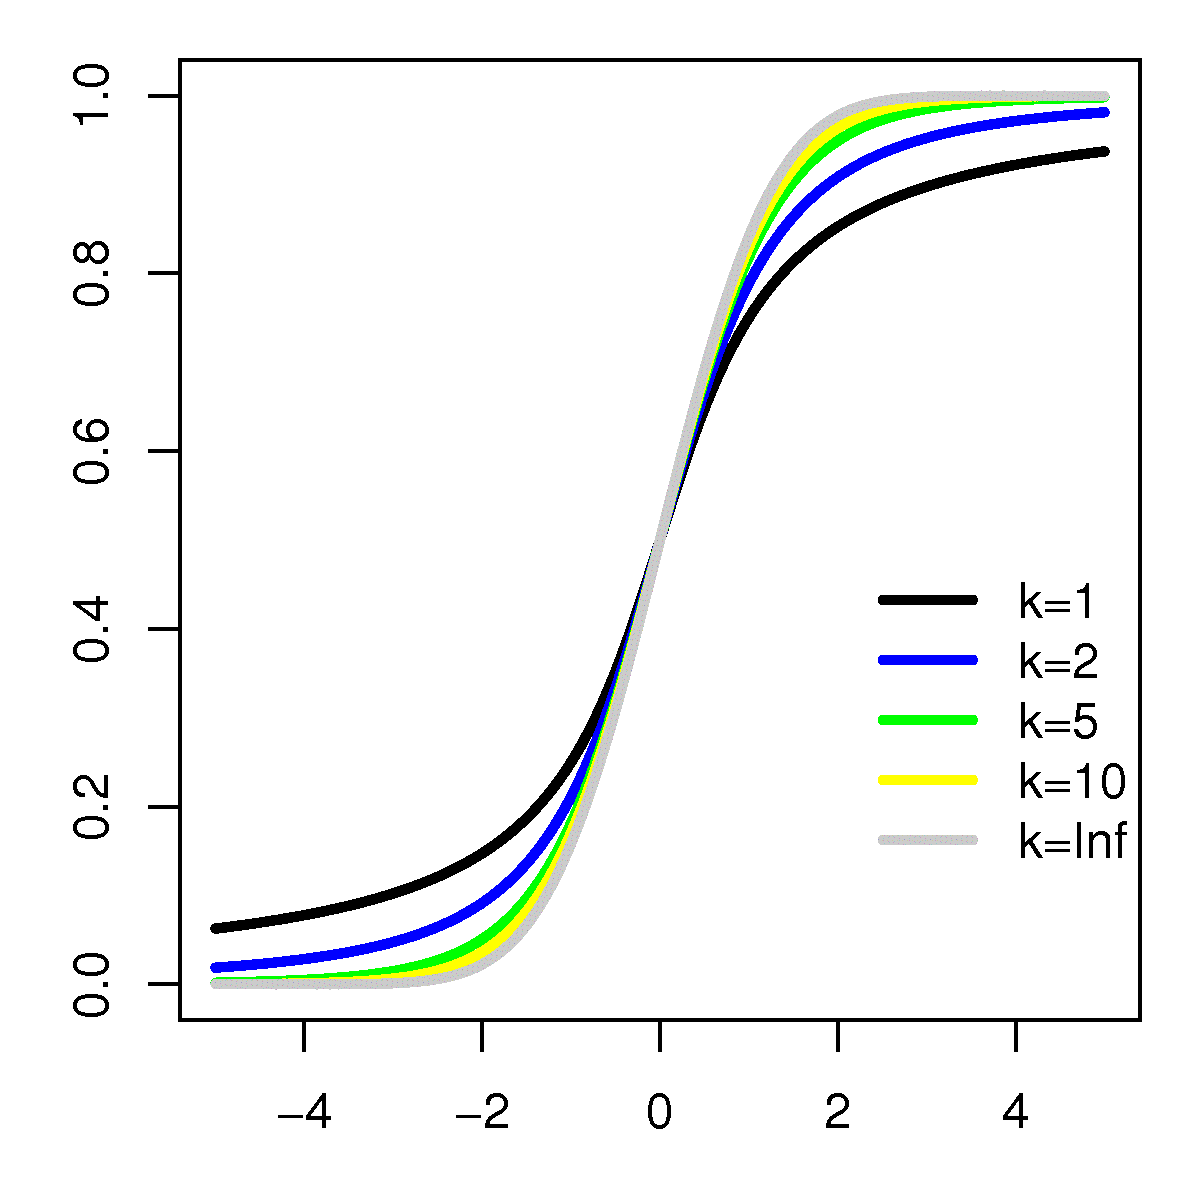
\includegraphics[height=5cm,keepaspectratio=true]{./images/T_distributionCDF.png}
	% T_distributionCDF.png: 0x0 pixel, 300dpi, 0.00x0.00 cm, bb=
	\caption{De Desconocido, CC BY-SA 3.0, https://commons.wikimedia.org/w/index.php?curid=788691}
	\label{fig:tCDF}
\end{figure}

\begin{lstlisting}[language=Python, caption=Distribución $t$ en \texttt{Python}]
	from scipy import stats
	import numpy as np
	import matplotlib.pyplot as plt
	
	def ft(x, nu):
	return stats.t.pdf(x, df=nu)
	def Ft(x, nu):
	return stats.t.cdf(x, df=nu)
	x = np.arange(-4,4,0.01)
	yd = ft(x,30)
	yc = Ft(x,30)
	
	fig, ax = plt.subplots()
	plt.plot(x, yd, 'r', linewidth=2)
	plt.plot(x, yc, 'b', linewidth=2)
	plt.ylim(ymin=0)
	plt.show()
\end{lstlisting}



\begin{figure}
	\centering
	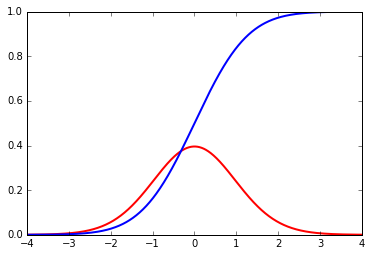
\includegraphics[height=7cm,keepaspectratio=true]{./images/tCDF.png}
	% tPDF.png: 0x0 pixel, 300dpi, 0.00x0.00 cm, bb=
\end{figure}



El parámetro \texttt{df} se le conoce como \emph{grados de libertad} y generalmente se denota como $\nu$ (la letra \texttt{nu} griega).


Si una variable aleatoria $X$ tiene distribución $t$ con $\nu$ grados de libertad, entonces
\begin{align}
	\mu_{X}=0, \; \s^{2}_{X}=\dfrac{\nu}{\nu-2}
\end{align}



\begin{ejemplo}
	Consideremos una variable con distribución $t$ y $\nu=9$ grados de libertad. Encuentre el valor de $t$ para el cuál el área a la derecha sea $0.05$ pero el total del área sin sombrear sea $0.90$.
	\begin{figure}
		\centering
		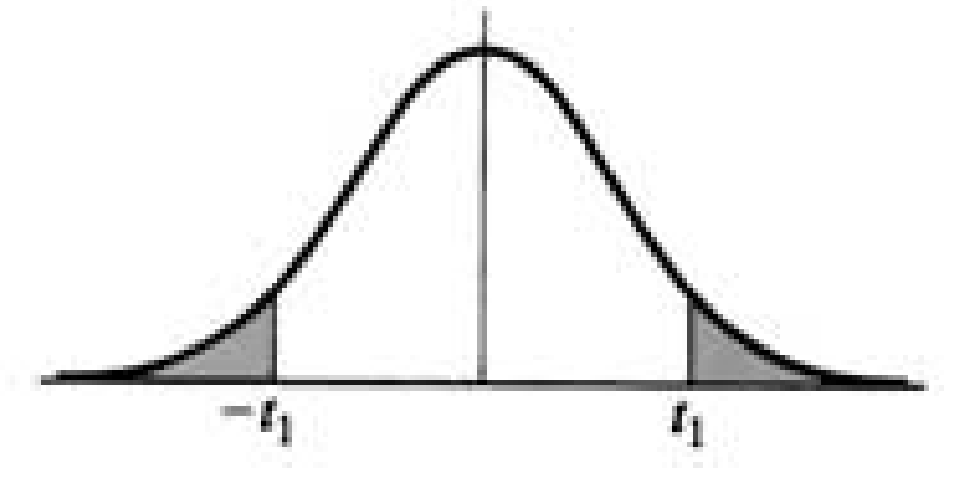
\includegraphics[height=3cm,,keepaspectratio=true]{./images/tExample.png}
		% tExample.png: 0x0 pixel, 300dpi, 0.00x0.00 cm, bb=
	\end{figure}
	
\end{ejemplo}


[]{tExample.py}
\begin{lstlisting}[language=Python]
	from scipy import stats
	import numpy as np
	import matplotlib.pyplot as plt
	
	def tp(x, nu):
	return stats.t.ppf(x, df=nu)
	
	print tp(0.05, 9)
	##-1.83311293265
	print tp(1-0.05, 9)
	##1.83311293265
\end{lstlisting}

\paragraph{Varianza muestral}
\begin{align}
	S^{2}=\sum\dfrac{\left( A_{i}-A_{0} \right)^{2}}{n-1}
\end{align}


\paragraph{Estadístico t}
\begin{align}
	t = \dfrac{\left( A-A_{0} \right)}{S/\sqrt{n}}
\end{align}



\section{Intervalos de confianza, niveles de significación y valores $p$}

\begin{figure}
	\centering
	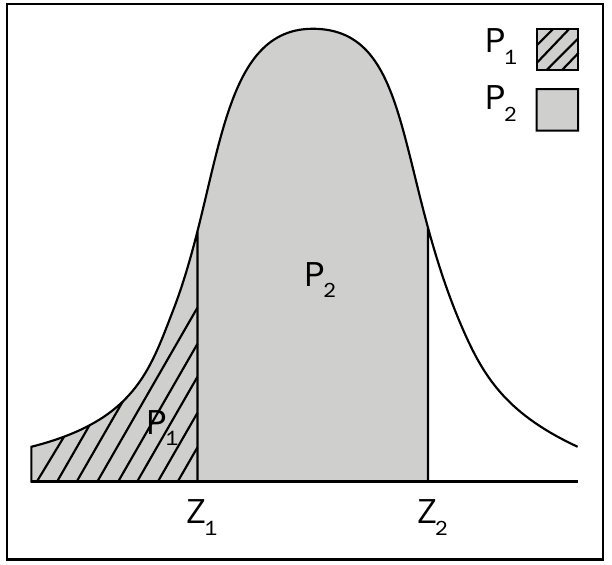
\includegraphics[height=5cm,keepaspectratio=true]{./images/kum0401.png}
	% kum0401.png: 0x0 pixel, 300dpi, 0.00x0.00 cm, bb=
	\caption{Una distribución típica normal con valores $p.$}
	\label{fig:0401}
\end{figure}



Supongamos que $Z_{1}$ y $Z_{2}$ son dos $Z-$estadísticos correspondientes a dos valores de una variable aleatoria y $p_{1}$ y $p_{2}$ son áreas encerradas por la curva de densidad a la derecha de esos valores.

En otras palabras
\begin{align}
	P(X>Z_{1})=p_{1}\\
	P(X>Z_{2})=p_{2}
\end{align}



Entonces, podemos definir un intervalo en el cual encontrar el valor de una variable aleatoria, al cual llamaremos \emph{intervalo de confianza.}


Por ejemplo, para una distribución normal con media $\mu$ y desviación estándar $\sigma,$ el valor de la variable aleatoria estará en el \emph{intervalo} $[\mu-3\s,\mu+3\sigma]$ con una \emph{confianza} (problemaabilidad) del $99\%.$


Para cualquier \emph{estimador} (variable aleatoria) que tenga una distribución normal, uno puede definir un intervalo de confianza si decidimos el nivel de confianza o problemaabilidad.


Podemos pensar en los \emph{intervalos de confianza} cómo el umbral de los valores aceptados para sostener que la \emph{hipótesis nula} es cierta


Si el valor del estimador vive en este rango, será estadísticamente correcto decir que la hipótesis nula es correcta.


Para definir un intervalo de confianza, se necesita definir antes un \emph{nivel (o problemaabilidad) de confianza.}  Esta problemaabilidad necesita ser definida por el investigador dependiendo del contexto.


Digamos que esta problemaabilidad es $p$. En general, utilizaremos el \emph{nivel de significación}
\begin{align}
	\beta = 1-p,
\end{align}
que representa la problemaabilidad de que la hipótesis nula no sea correcta. 

$\beta$ es definida por el investigador y usualmente esta en el orden de $0.01$ a $0.1$.



Un concepto importante que aprender aquí es el \emph{valor de problemaabilidad} o simplemente \emph{valor-}$p$ de un estadístico:  Es la problemaabilidad de que una variable aleatoria asuma un valor mayor al \emph{valor-}$Z$ (o al \emph{valor-}$t$)
\begin{align}
	p-\texttt{valor}=P\left( X>Z \right)
\end{align}



\begin{figure}
	\centering
	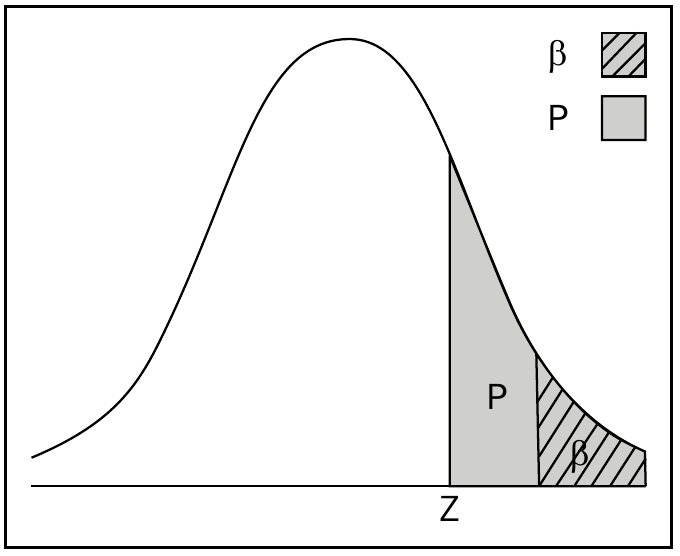
\includegraphics[height=5cm,keepaspectratio=true]{./images/kum0402.png}
	% kum0402.png: 0x0 pixel, 300dpi, 0.00x0.00 cm, bb=
	\caption{Una distribución normal típica con $p-$valores y nivel de significación.}
	\label{fig:0402}
\end{figure}


\subsection{Criterio}
\begin{itemize}
	\item Aceptar la \emph{hipótesis nula y rechazar la alternativa si $p-\texttt{valor}>\beta$}
	\item Aceptar la \emph{hipótesis alternativa y rechazar la nula si $p-\texttt{valor}<\beta$}
\end{itemize}



Debido a la simetría de la distribución normal, existen tres tipos de pruebas de hipótesis:
\begin{enumerate}
	\item Cola izquierda;
	\item cola derecha;
	\item ambas colas.
\end{enumerate}


\subsection{Cola izquierda}
\begin{figure}
	\centering
	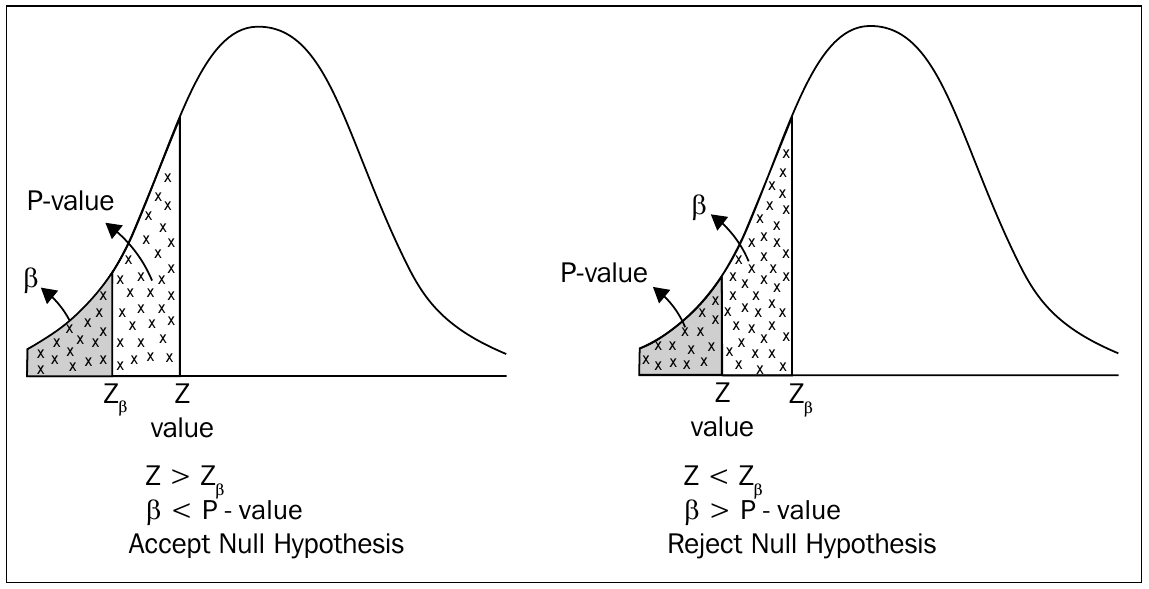
\includegraphics[width=10cm,keepaspectratio=true]{./images/kum0403.png}
	% kum0403.png: 0x0 pixel, 300dpi, 0.00x0.00 cm, bb=
	\caption{Prueba de hipótesis: Cola izquierda}
	\label{kum0403}
\end{figure}


\subsection{Cola derecha}
\begin{figure}
	\centering
	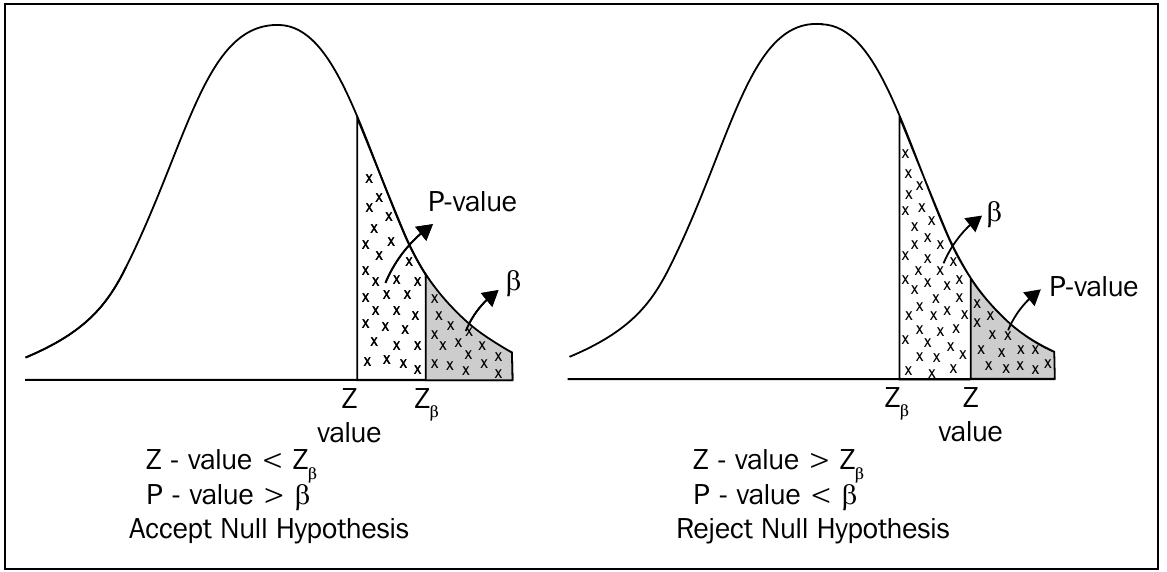
\includegraphics[width=10cm,keepaspectratio=true]{./images/kum0404.png}
	% kum0403.png: 0x0 pixel, 300dpi, 0.00x0.00 cm, bb=
	\caption{Prueba de hipótesis: Cola derecha}
	\label{kum0403}
\end{figure}


\subsection{Dos colas}
Analizamos ambas colas y si en alguna de las dos colas, falla la respectiva prueba de hipótesis, la prueba de hipótesis se rechaza.


\section{Una guía paso a paso para realizar una prueba de hipótesis}
\subsection{Paso \#1}
\emph{Defina sus hipótesis nula y alternativa.} Las hipótesis nula es algo que ya se establece y se acepta como cierto, al cuál denotamos como $H_{0}.$ También, suponemos que el valor del parámetro en la hipótesis nula es $A_{0}.$

\subsection{Paso \#2}
Tome una muestra, digamos de unas 100 o 1000 personas o ocurrencias de eventos, y calcule el valor del estimador (por ejemplo, el promedio del parámetro como es la edad promedio, el tiempo promedio de entrega de la pizza, ingreso promedio, etc.) Digamos que este valor fue $A_{m}.$

\subsection{Paso \#3}
Calcule el valor normal estándar del valor $Z$
\begin{align}
	Z=\dfrac{A_{m}-A_{0}}{\s/\sqrt{n}}
\end{align}



En la fórmula anterior, $\s$ es la desviación estándar de la población o ocurrencias de eventos y $n$ es el número de personas en la muestra.


La probleamibilidad asociada con el valor $Z$ calculada en el paso $3$ se debe comparar con el nivel de significación de la prueba a determinar si la hipótesis nula será aceptada o rechazada.

\subsection{Ejemplo}
Un famoso restaurante de pizza afirma que su tiempo de entrega es de \emph{20 minutos}, con una desviación estándar de 3 minutos. 

Un investigador de mercados independiente afirma que ellos están desinflando los números para ganar clientes y el tiempo de entrega promedio es de hecho \emph{21.2 minutos}.

¿Es su afirmación justificada o está el negocio de pizza correcto en su afirmación? \emph{Suponga un nivel de significación del $5\%$}


Definamos las hipótesis nula y alternativa:
\begin{itemize}
	\item Lo que el negocio de pizzas afirma: $H_{0}:A_{0}=20.$
	\item Lo que el investigador reclama:
	$H_{a}: A_{0}>20.$
	\item Desviación estándar (conocida): $\s=3.$
	\item Tamaño de la muestra: $n=64.$
	\item Nivel de significación: $\beta=0.05.$
\end{itemize}


Calculemos el valor $Z$:
\begin{align}
	Z=\dfrac{21.2-20}{3/\sqrt{64}}=3.2
\end{align}



Denotemos por $F$ la función de distribución acumulativa de una variable normal $N(0,1).$ 

Calculamos el valor $p$ correspondiente al valor $Z=3.2$:
\begin{align}
	\texttt{valor-p}&=1 - F(3.2)\\
	&=1-0.999312862062\\
	&= 0.000687137937916
\end{align}



Esto significa que si la media fuera $A_{0}=20,$ la problemaabilidad de que la media muestral fuera $A=21.2$ es $\approx 0.069\%.$


Como \emph{elegimos} un nivel de significación $\beta=5\%,$ y $0.069\% < 5\%,$ podemos rechazar la hipótesis nula $H_{0}: A_{0}=20.$


\begin{figure}
	\centering
	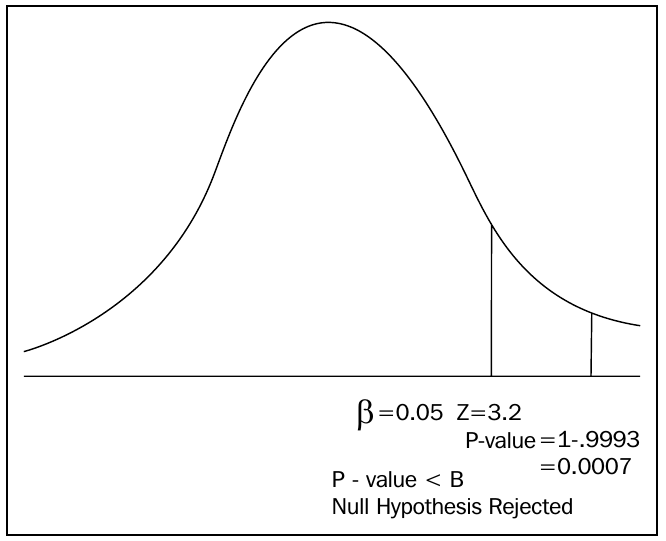
\includegraphics[height=5cm,keepaspectratio=true]{./images/kum0405.png}
	% kum0405.png: 0x0 pixel, 300dpi, 0.00x0.00 cm, bb=
	\caption{La hipótesis nula se rechaza porque el $p-$valor es menor al nivel de significación $\beta$.}
	\label{fig:0405}
\end{figure}


\section{Prueba $\chi-$cuadrada}

La \emph{prueba $\chi^{2}$} se usa comúnmente para comparar \emph{datos observados vs datos esperados} suponiendo que los datos siguen ciertas hipótesis.


Debemos suponer cierta hipótesis, la cuál nuestros datos seguirán y calculamos los datos esperados de acuerdo a esa hipótesis.


Debemos ya tener los datos observados, y calcular la desviación entre estos y los esperados usando el estadístico definido en la siguiente fórmula:
\begin{align}
	\texttt{valor }\chi^{2}\texttt{:} g= \sum\dfrac{\left( O-E \right)^{2}}{E},
\end{align}
donde $O$ es el valor observado y $E$ el esperado, con la suma sobre todos los posibles datos.

\paragraph{Aplicaciones del estadístico $\chi-$cuadrada}
La prueba de ji cuadrado se puede usar para hacer lo siguiente:
\begin{itemize}
	\item Mostrar una relación causal o independencia entre una variable de entrada y otra de salida.  
	\item Verificar si los datos observados provienen de una fuente justa / imparcial. 
	\item Comproblemaar si los datos son demasiado buenos para ser verdad.
\end{itemize}


\paragraph{Ejemplo}
Realicemos un experimento hipotético en el que una moneda se lanza 10 veces. ¿Cuántas veces espera obtener ya sea un reverso o un sol?  La respuesta adecuada sería 5.  Ahora bien, ¿qué pasaría si realizamos este experimento 1000 veces y registramos los números de reversos y soles.


Supongamos que observamos soles 553 veces y reversos el resto de ocasiones:
\begin{center}
	$H_{0}:$ La proporción de soles y reversos es $0.5$ \\
	$H_{a}:$ La proporción no es $0.5$
\end{center}



\begin{center}
	\begin{tabular}{|l|l|l|}\hline
		& Soles & reversos\\\hline
		Observado & 553 & 447\\\hline
		Esperado & 500 & 500\\\hline
	\end{tabular}
\end{center}


Calculemos el valor $\chi^{2}:$
\begin{align}
	g = \dfrac{\left( \left( 553-500 \right)^{2}+\left( 447-500 \right)^{5} \right)}{500}\approx 11.236
\end{align}



Este valor$-\chi^{2}$ se compara al valor en una \emph{distribución $\chi^{2}$} para un número dado de \emph{grados de libertad} y un nivel de significación.

\paragraph{La Distribución $\chi^{2}$}
Sean $X_{1},X_{2},...,X_{\nu}$ variables aleatorias independientes $N(0,1).$
Consideremos la variable aleatoria
\begin{align}
	\label{outline:19}
	\chi^{2}=X_{1}^{2}+...+X_{\nu}^{2}
\end{align}
a la que llamaremos \emph{chi cuadrada.} Su correspondiente distribución de problemaabilidad recibe el mismo nombre.

\paragraph{Propiedades de $\chi^{2}$}
\begin{align}
	\label{eq:22}
	\mu=\nu, \; \s = 2\nu
\end{align}


[]{scipy.stats.chi2}
\begin{lstlisting}[language=Python]
	from scipy.stats import chi2
	import numpy as np
	import matplotlib.pyplot as plt
	fig, ax = plt.subplots(1, 1)
	
	df = 55
	
	x = np.linspace(chi2.ppf(0.01, df),
	chi2.ppf(0.99, df), 100)
	ax.plot(x, chi2.pdf(x, df),'r-',
	lw=5, alpha=0.6, label='chi2 pdf')
\end{lstlisting}



\begin{figure}
	\centering
	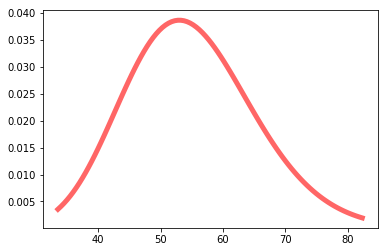
\includegraphics[height=5cm,keepaspectratio=true]{./images/statsChi2.png}
	% statsChi2.png: 0x0 pixel, 300dpi, 0.00x0.00 cm, bb=
	\caption{Función de densidad de distribución $\chi^2$ con $\nu=55$}
	\label{fig:Chi2}
\end{figure}


[]{\texttt{statsChi2.py}}
\begin{lstlisting}[language=Python]
	from scipy.stats import chi2
	import numpy as np
	import seaborn as sns
	import matplotlib.pyplot as plt
	
	sns.set_palette("husl")
	fig, ax = plt.subplots(1, 1)
	
	for df in range(2,15+1):
	x = np.linspace(chi2.ppf(0.01, df),
	chi2.ppf(0.99, df), 100)
	ax.plot(x, chi2.pdf(x, df), label='chi2 pdf')
\end{lstlisting}



\begin{center}
	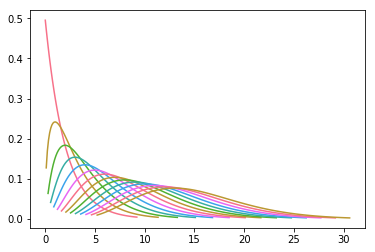
\includegraphics[height=7cm,keepaspectratio=true]{./images/statsChi2Several.png}
	% statsChi2Several.png: 0x0 pixel, 300dpi, 0.00x0.00 cm, bb=
\end{center}


\paragraph{Regresando a nuestro ejemplo...}
El número de grados de libertad es el número de categorías menos uno.  En nuestro ejemplo $\nu = 2-1 =1.$  Supongamos un nivel de significación $\beta=0.05.$


\begin{figure}
	\centering
	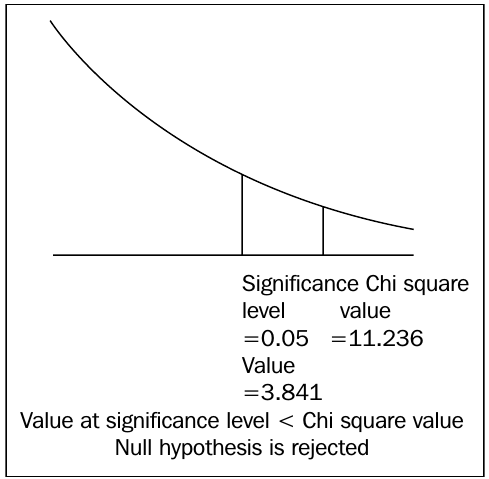
\includegraphics[height=5cm,keepaspectratio=true]{./images/kum0407.png}
	% kum0407.png: 0x0 pixel, 300dpi, 0.00x0.00 cm, bb=
	\caption{La hipótesis nula se rechaza porque el valor del estadístico $\chi^2$ al nivel de significación es menor que el valor del estadístico.}
	\label{fig:0407}
\end{figure}


[]{Otro ejemplo}
Examinemos otros ejemplo donde queremos demostrar que el género de un estudiante y las materias que escoge son independientes.


Supongamos que un grupo de estudiantes, la siguiente tabla representa el número de hombres y mujeres que toman matemáticas, arte y comercio como sus materias principales.


\begin{center}
	\begin{tabular}{|l|l|l|l|l|}\hline
		& Matemáticas & Artes & Comercio & Total\\\hline
		Hombres & 68 & 52 & 90 & 210\\\hline
		Mujeres & 28 & 37 & 35 & 100\\\hline
		Total & 106 & 89 & 125 & 310\\\hline
	\end{tabular}
\end{center}



Si en la elección de las materias, no fuera relevante el género, entonces el número esperado de hombres y mujeres tomando diferentes materias sería
\begin{center}
	\begin{tabular}{|l|l|l|l|l|}\hline
		& Matemáticas & Arte & Comercio & Total\\\hline
		Niños &  &  &  & \\\hline
		Niñas &  &  &  & \\\hline
		Total &  &  &  & \\\hline
	\end{tabular}
\end{center}



Las desviaciones se calculan usando la fórmula
$(O-E)^2/E$:
\begin{center}
	\begin{tabular}{|l|l|l|l|l|}\hline
		& Matemáticas & Arte & Comercio & Total\\\hline
		Hombres &  &  &  & \\\hline
		Mujeres &  &  &  & \\\hline
		Total &  &  &  & \\\hline
	\end{tabular}
\end{center}

El estadístico $\chi^{2}$ se obtiene al sumar todos estos valores.

\paragraph{Conclusiones (del profesor)}
Como $\chi^{2}= 4.99$ y el valor del estadístico $\chi^{2}$ a un nivel se significación es $11.07,$ la hipótesis nula se acepta.

De manera equivalente
\begin{align}
	\texttt{valor-}p=1- F_{\chi^{2}}(4.99)=0.416991040312>\beta=0.05,
\end{align}
obtenemos la misma conclusión:
\begin{center}
	\emph{La elección de materias es independiente del género.}
\end{center}



\section{Correlación}

La correlación es la premisa de la modelación predictiva, en el sentido de que es un factor con base en el cuál podemos predecir resultados.


Una buena correlación entre dos variables sugiere que existe una suerte de dependencia entre ambas:  Si una cambia, la otra también lo hará. 

Podemos decir que una buena correlación asegura una relación matemática entre dos variables y debido a esto, seremos capaces de predecir su comportamiento.


La relación puede ser de cualquier tipo.  Si $x$ y $y$ son dos variables correlacionadas, entonces podemos escribir:
\begin{align}
	Y=f(X)
\end{align}

\paragraph{Ejemplos de correlación}
\begin{itemize}
	\item Correlación lineal
	\begin{align}
		y = ax+b
	\end{align}
	\item Correlación exponencial
	\begin{align}
		y = be^{ax}
	\end{align}
\end{itemize}


\paragraph{Definición de correlación} Si $X,Y$ son dos variables aleatorias discretas, que pueden tomar valores $\set{x_{0},x_{1},...}$ y $\set{y_{0},y_{1},...}$, con promedios $\bar{x}, \bar{y}$  respectivamente, su correlación se define como
\begin{align}
	\corr(X,Y) = \dfrac{\sum_{x_{i},y_{j}}
		\left( \left( x_{i}-\bar{x} \right)\left( y_{j}-\bar{y} \right) \right)}
	{\sqrt{\sum_{x_{i},y_{j}}
			\left( x_{i}-\bar{x} \right)^{2}\sum_{x_{i},y_{j}}
			\left( y_{i}-\bar{y} \right)^{2}}}
\end{align}



\paragraph{Propiedades de la correlación}
\begin{itemize}
	\item El valor del coeficiente de correlación está entre $-1$ y $1$, es decir $-1\leq  \corr(X,Y)  \leq 1.$ 
	\item Una correlación positiva significa una relación directa entre las dos variables. 
	\item Una correlación negativa significa una relación inversa entre las dos variables. 
	\item Entre mayor sea la magnitud del coeficiente, más fuerte será la relación entre variables.
\end{itemize}


\paragraph{¡Advertencia!}
Aunque una correlación fuerte sugiere algún tipo de relación que puede ser utilizada para la predicción del comportamiento de una variable respecto de otra, \emph{esto no implica que dicha relación sea el único factor que explique dicho comportamiento.}


\begin{observacion}
	\emph{¡Correlación no implica causalidad!}
\end{observacion}



Por ejemplo, existe una correlación positiva muy fuerte entre el número de palabras que conoce un ser humano y el número de calzado que utiliza...  Pero esto esto se explica porque a medida que el ser humano crece, necesita zapatos más grandes y aprende palabras nuevas. 

\emph{¡No quiere decir que si utilizas un número más grande serás más culto!}


Tratemos de entender mejor este concepto mirando una base de datos y tratando de encontrar una correlación entre sus variables.  La base de datos que estaremos observando es una muy popular sobre los costos varios incurridos en \emph{publicidad por diferentes medios} y \emph{ventas de un producto en particular.}


Posteriormente, utilizaremos el método conocido como \emph{regresión lineal} para explorar estos mismo datos.

Por ahora, importemos esta base de datos y calculemos los coeficientes de correlación:

[,]{\texttt{advertising.py}}
\begin{lstlisting}[language=Python]
	#!/usr/bin/env python3
	# -*- coding: utf-8 -*-
	
	import pandas as pd
	
	advert = pd.read_csv("./dataBases/Advertising.csv")
	print(advert.head())
	
	import numpy as np
	
	advert["dX*dY"] = ( advert["TV"] -
	np.mean(advert["TV"])) * ( advert["Sales"]
	np.mean(advert["Sales"]))
	advert["dX**2"] = ( advert["TV"] -
	np.mean(advert["TV"])) ** 2
	advert["dY**2"] = ( advert["Sales"] -
	np.mean(advert["Sales"])) ** 2
	
	sxy = advert.sum()["dX*dY"]
	sxx = advert.sum()["dX**2"]
	syy = advert.sum()["dY**2"]
	
	r = sxy/np.sqrt(sxx*syy)
\end{lstlisting}


[,]{Salida de la pantalla}
\begin{lstlisting}[language=Python]
	TV  Radio  Newspaper  Sales
	0  230.1   37.8       69.2   22.1
	1   44.5   39.3       45.1   10.4
	2   17.2   45.9       69.3    9.3
	3  151.5   41.3       58.5   18.5
	4  180.8   10.8       58.4   12.9
\end{lstlisting}



[,]{\texttt{advertising2.py}}
\begin{lstlisting}[language=Python]
	#!/usr/bin/env python3
	# -*- coding: utf-8 -*-
	
	import pandas as pd
	
	advert = pd.read_csv("./dataBases/Advertising.csv")
	print(advert.head())
	
	import numpy as np
	
	def rCoef(df, var1, var2):
	df["dX*dY"] = (df[var1]-np.mean(df[var1]))*(df[var2]-np.mean(df[var2]))
	df["dX**2"] = (df[var1]-np.mean(df[var1]))**2
	df["dY**2"] = (df[var2]-np.mean(df[var2]))**2
	sxy = df.sum()["dX*dY"]
	sxx = df.sum()["dX**2"]
	syy = df.sum()["dY**2"]
	r = sxy/np.sqrt(sxx*syy)
	return r
	
	tvVsSales = rCoef(advert, "TV", "Sales")
	## 0.782224424862
	radioVsSales = rCoef(advert, "Radio", "Sales")
	## 0.576222574571
\end{lstlisting}




\begin{figure}
	\centering
	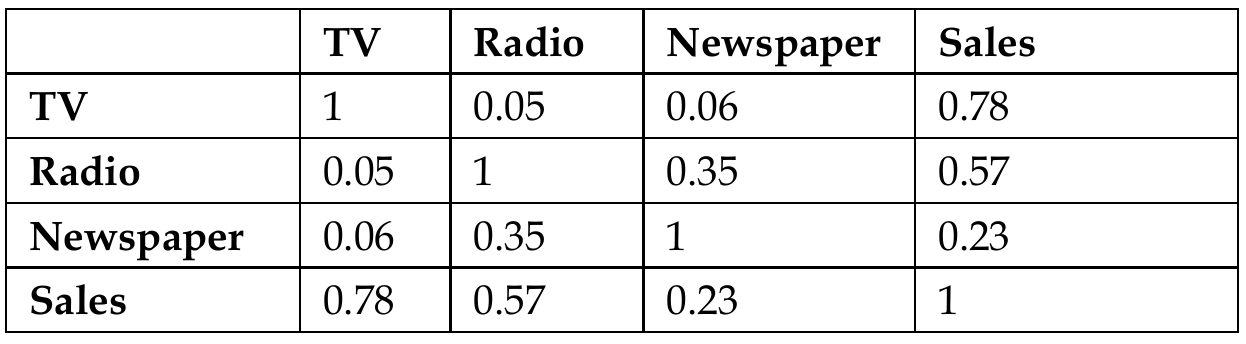
\includegraphics[width=10cm,keepaspectratio=true]{./images/correlationMatrix.png}
	% correlationMatrix.png: 0x0 pixel, 300dpi, 0.00x0.00 cm, bb=
	\caption{Matriz de correlación}
	\label{correlationMatrix}
\end{figure}



Veamos la naturaleza de esta correlación graficando las variables \texttt{TV}, \texttt{Radio} y \texttt{Newspaper} vs \texttt{Sales} del \textit{data frame} \texttt{advert}.

[,]{tvVsSales.py}
\begin{lstlisting}[language=Python]
	#!/usr/bin/env python3
	# -*- coding: utf-8 -*-
	
	import pandas as pd
	advert = pd.read_csv("./dataBases/Advertising.csv")
	
	import matplotlib.pyplot as plt
	
	plt.plot(advert['TV'],advert['Sales'],'ro')
	plt.title('TV vs Sales')
	plt.show()
	
	plt.plot(advert['Radio'],advert['Sales'],'ro')
	plt.title('Radio vs Sales')
	plt.show()
	
	plt.plot(advert['Newspaper'],advert['Sales'],'ro')
	plt.title('Newspaper vs Sales')
	plt.show()
\end{lstlisting}


\begin{center}
	\includegraphics[width=10cm,keepaspectratio=true]{./images/tvVsSales.png}
	% tvVsSales.png: 0x0 pixel, 300dpi, 0.00x0.00 cm, bb=
\end{center}


\begin{center}
	\includegraphics[width=10cm,keepaspectratio=true]{./images/radioVsSales.png}
	% tvVsSales.png: 0x0 pixel, 300dpi, 0.00x0.00 cm, bb=
\end{center}


\begin{center}
	\includegraphics[width=10cm,keepaspectratio=true]{./images/newsVsSales.png}
	% tvVsSales.png: 0x0 pixel, 300dpi, 0.00x0.00 cm, bb=
\end{center}


%%%%%%%%%%%%%%%%%%%%%%%%%%%%%%%
\chapter{Regresiones lineales}
\section{Introducción}

En esta unidad, trataremos con una técnica básica de modelación predictiva llamada \emph{regresión lineal}, la cuál permite crear un modelo a partir de una base de datos histórica.


Nuestro propósito es entender las matemáticas detrás de la regresión lineal e ilustrar sus resultado a través de su implementación en varias bases de datos.

\subsection{Mapa de ruta}
\begin{itemize}
	\item Las matemáticas detrás de la regresión lineal.
	\item Implementación de la regresión lineal con Python.
	\item Interpretación de los parámetros resultantes.
	\item Validación del modelo.
	\item Manejo de Problemas relacionados con regresión lineal.
\end{itemize}


\subsection{Modelos matemáticos}
Un \emph{modelo matemático/estadístico/predictivo} es una ecuación matemática que consiste en \emph{entradas} que producen \emph{salidas} cuando el valor de las variables entrantes se introduce en el modelo.

\subsection{Ejemplo}
Por ejemplo, supongamos que el precio $P$ de una casa es \emph{linealmente dependiente} en su tamaño $S$, comodidades $A$ y disponibilidad de transporte $T$.



La ecuación correspondiente sería
\begin{align}
	P = a_{1}\times S+ a_{2} \times A + a_{3} \times T
\end{align}



Esta ecuación es llamado el \emph{modelo} y los coeficientes $a_{1},a_{2},a_{3}$ son sus parámetros.



La variable $P$ es resultado predicho, mientras que $S,A,T$ con las variables de entrada, que son datos conocidos.


Sin embargo, los parámetros $a_{i}$ deben ser estimados a partir de los datos históricos.


Una vez que estos parámetros son determinados, el modelo está listo para ser problemaado.


\section{Entendiendo las matemáticas detrás de la regresión lineal}

Supongamos que tenemos una base de datos hipotética que contiene la información acerca del costo (en unidades de $\$10000$) de varias casas y sus respectivos tamaños (en pies cuadrados $ft^{2}$).


\begin{center}
	\begin{tabular}{|l|l|}\hline
		Tamaño & Costo\\\hline
		1500 & 45\\\hline
		1200 & 38\\\hline
		1700 & 48\\\hline
		800 & 27\\\hline
	\end{tabular}
\end{center}



En este caso, el costo es la variable de salida, mientras que el tamaño es la variable de entrada. 

La entrada y la salida generalmente se denotan por $X$ y $Y$, respectivamente.


En el caso de la regresión lineal, supondremos que el costo $Y$ es una función lineal de tamaño $X$ y para estimar $Y,$ proponemos el modelo \begin{align}
	Y_{e} = \a + \beta X ,
\end{align}
donde $Y_{e}$ es el \emph{valor estimado} de $Y$ con base en nuestra ecuación lineal.


\begin{observacion}
	El propósito de la regresión lineal es encontrar valores $\alpha, \beta$ estadísticamente significativos, que \emph{minimicen} la diferencia entre $Y$ y $Y_{e}.$
\end{observacion}



En el caso de nuestro ejemplo, si encontramos los valores de $\a=2$ y $\beta=0.03,$ entonces la ecuación será
\begin{align}
	Y_{e}= 2 + 0.03 X.
\end{align}


Usando esta ecuación, podemos estimar el costo una casa de cualquier tamaño.  Por ejemplo, para una casa de $900 ft^{2}$, el costo será
\begin{align}
	Y_{e}= 2 + 0.03(900)= 29 .
\end{align}


La siguiente pregunta que nos haremos es como estimar $\a$ y $\beta.$  Para esto usaremos un método llamado suma de  \emph{mínimos cuadrados} para la diferencia entre $Y$ y $Y_{e},$ que representaremos como
\begin{align}
	\ep = Y-Y_{e}.
\end{align}



Nuestro objetivo es minimizar
\begin{align}
	\sum \ep^{2} & = \sum \left( Y-Y_{e} \right)^{2}\\
	&= \sum \left( Y - \left( \a+\beta X \right) \right)^{2}
\end{align}
respecto de los parámetros $\a, \beta.$


Utilizando un poco de cálculo, se puede demostrar que los valores de los parámetros que minimizan la suma anterior son
\begin{align}
	\label{beta}
	\beta &= \dfrac{\sum \left( x-\bar{x} \right)\left( y-\bar{y} \right)}{\sum\left( x-\bar{x} \right)^{2}}\\
	\label{alfa}
	\a &= \bar{y}-\beta\times \bar{x}
\end{align}

% \part{NO BORRAR}
% \section{Recursos}
% \subsection{analisisPredictivo}
% El repositorio con los scripts de \texttt{Python 3} de esta presentación los puede encontrar en \href{https://github.com/julihocc/ulsaPye/tree/master/analisisPredictivo}{https://github.com/julihocc/ulsaPye/tree/master/analisisPredictivo}
% 
% [t, ]
% \frametitle{Referencias}
% \nocite{*}
% \betaibliographystyle{amsalpha}
% \betaibliography{ulsaPye}
% 
\section{Regresión lineal usando datos simulados}

Para propósitos de regresión lineal, escribimos $Y_{e}=\a+\beta X,$ aunque $Y$ rara vez será lineal y podría tener un componente de error o residual, y en ese caso escribimos
\begin{align}
	Y=\a + \beta X + K.
\end{align}


En la ecuación anterior, $K$ es el error, el cuál es una variable aleatoria que supondremos está normalmente distribuida.


Simulemos los datos para $X$ y $Y$ y tratemos de observar como es que los valores estimados $\left( Y_{e} \right)$ difieren del valor real $\left( Y \right)$.


Para $X,$ generamos 100 números aleatorios normalmente distribuidos con media $1.5$ y desviación estándar $2.5$ (pero usted puede tomar otro par de números y experimentar.)


\paragraph{Consideraciones}
\begin{enumerate}
	\item Para el valor $(Y_{e}),$ supondremos una ordenada al origen $\a=2$ y una pendiente $\beta=0.3$. 
	
	\item
	Posteriormente, calcularemos los valores óptimos de $\a$ y $\beta$, usando los datos simulados y veremos como cambia la eficacia del modelo.
	
	\item
	Para el valor actual $Y$, adicionamos un término residual, que no es otra cosa que una variable normalmente distribuida con media $\mu=0$ y desviación estándar de $\sigma=0.5$.
\end{enumerate}


[,]{\texttt{fittingLinearRegression.py}}
\begin{lstlisting}[language=Python]
	import pandas as pd
	import numpy as np
	
	np.random.seed(1234)
	
	x=2.5*np.random.randn(100)+1.5
	res=.5*np.random.randn(100)+0
	ypred=2+.3*x
	yact=2+.3*x+res
	xlist=x.tolist()
	ypredlist=ypred.tolist()
	yactlist=yact.tolist()
	df=pd.DataFrame({'Input_Variable(X)':xlist,'Predicted_Output(ypred)':ypredlist,'Actual_Output(yact)':yactlist})
	print(df.head())
	
	
	import matplotlib.pyplot as plt
	
	% x=2.5*np.random.randn(100)+1.5
	% res=.5*np.random.randn(100)+0
	% ypred=2+.3*x
	% yact=2+.3*x+res
	
	ymean=np.mean(yact)
	yavg=[ymean for i in range(1,len(xlist)+1)]
	
	plt.plot(x,ypred)
	plt.plot(x,yact,'ro')
	plt.plot(x,yavg)
	plt.title('Actual vs Predicted')
\end{lstlisting}

[,]{} 
\begin{lstlisting}[language=Python]
	Actual_Output(yact)  Input_Variable(X)  Predicted_Output(ypred)
	0             2.949179           2.678588                 2.803576
	1             1.840035          -1.477439                 1.556768
	2             3.776326           5.081767                 3.524530
	3             2.358159           0.718370                 2.215511
	4             2.151703          -0.301472                 1.909558
\end{lstlisting}


\begin{center}
	\includegraphics[width=10cm,keepaspectratio=true]{./images/actualVsPredicted.png}
	% actualVsPredicted.png: 0x0 pixel, 300dpi, 0.00x0.00 cm, bb=
\end{center}



En la gráfica anterior, la linea horizontal representa la \emph{media} de los datos.


En caso de que no tuviéramos algún otro modelo predictivo, nuestra mejor elección sería la \emph{media aritmética}.


Otro punto para pensar es en como juzgar la eficiencia de nuestro modelos. 

Si usted pasa cualquier dato conteniendo dos variables, una de entrada y otra de salida, el programa de estadística generara algunos valores $\a,\beta.$



¿Pero cómo entender que esos valores que se nos están dando son un buen modelo?

\paragraph{Suma de Cuadrados Total}
\begin{align}
	SST = \sum\left( Y_{i}-\bar{Y} \right)^{2}
\end{align}

donde $\bar{Y}$ es el valor promedio de $Y_{1}, Y_{2},...$, los valores reales de $Y.$


\paragraph{Suma de Cuadrados de Regresión}

\begin{align}
	SSR = \sum\left( Y_{e,i}-\bar{Y} \right)^{2}
\end{align}
donde $\bar{Y}$ es el valor promedio de $Y_{1}, Y_{2},...$, los valores reales de $Y,$ mientras que $Y_{e,i}$ son los valores predichos por el modelos para cada $Y_{i}.$


\paragraph{Suma de Cuadrados de Diferencia}
\begin{align}
	SSD = \sum\left( Y_{i}-Y_{e,i} \right)^{2}
\end{align}



Recordemos que $Y_{e}=\a + \beta X$, con $\beta$ definida por \eqref{beta} y $\a$ por \eqref{alfa}.



Utilizando estas identidad se puede demostrar que
\begin{align}
	SST = SSR +SSD.
\end{align}



\begin{itemize}
	\item $SSR$: diferencia explicada por el modelo;
	\item $SSD$: diferencia no explicada por el modelo;
	\item $SST$: error total.
\end{itemize}




\begin{observacion}
	Entre mayor sera la proporción de $SSR:SST$, mejor será el modelo.
\end{observacion}


\paragraph{Coeficiente de determinación}
\texttt{R-cuadrado: }
\begin{align}
	R^{2}=\dfrac{SSR}{SST}
\end{align}


Como $SSR\leq SST,$ entonces $0\leq R^{2} \leq 1$, y entre más cercano sea a $1$ mejor será el modelo.



$R^{2}$ es un buen indicador de que una regresión lineal será efectiva.


En el script \texttt{fittingLinearRegression.py}, podemos agregar el siguiente pedazo de código para calcular el valor $R^{2}$.

[,]{\texttt{rCuadrada.py}}
\begin{lstlisting}[language=Python]
	df['SSR']=(df['Predicted_Output(ypred)']-ymean)**2
	df['SST']=(df['Actual_Output(yact)']-ymean)**2
	SSR=df.sum()['SSR']
	SST=df.sum()['SST']
	SSR/SST
\end{lstlisting}


El valor obtenido es $a\approx 0.65$, que es algo bueno. Sin embargo, los valores $\a=2, \beta=0.3$ para $Y_{e}$ pueden que no sean los mejores.

\section{Encontrando el valor optimo de los coeficientes de una regresión lineal}

Regresemos a nuestro marco de datos \texttt{df}. La columna \texttt{Input\_Variable(X)} es la variable predictora. 
La variable \texttt{Actual\_Output(yact)}, como su nombre lo siguiere, es la variable de salida real.


Utilizando estas dos variables, podemos calcular los valores de $\a$ y $\beta$ de acuerdo a las fórmulas \eqref{alfa} y \eqref{beta}.  En el siguiente script, implementaremos estas fórmulas para obtener un modelo optimo de regresión lineal.

[,]{\texttt{optimalValue.py}}
\begin{lstlisting}[language=Python]
	#!/usr/bin/env python3
	# -*- coding: utf-8 -*-
	"""
	Created on Mon Oct 23 00:37:36 2017
	
	@author: jdk2py
	"""
	
	import pandas as pd
	import numpy as np
	
	np.random.seed(1234)
	
	x=2.5*np.random.randn(100)+1.5
	res=.5*np.random.randn(100)+0
	ypred=2+.3*x
	yact=2+.3*x+res
	xlist=x.tolist()
	ypredlist=ypred.tolist()
	yactlist=yact.tolist()
	df=pd.DataFrame({'Input_Variable(X)':xlist,'Predicted_Output(ypred)':ypredlist,'Actual_Output(yact)':yactlist})
	
	ymean=np.mean(yact)
	yavg=[ymean for i in range(1,len(xlist)+1)]
	
	import matplotlib.pyplot as plt
	
	xmean=np.mean(df['Input_Variable(X)'])
	ymean=np.mean(df['Actual_Output(yact)'])
	df['betan']=(df['Input_Variable(X)']-xmean)*(df['Actual_Output(yact)']-ymean)
	df['xvar']=(df['Input_Variable(X)']-xmean)**2
	betan=df.sum()['betan']
	betad=df.sum()['xvar']
	beta=betan/betad
	alpha=ymean-beta*xmean
	print(beta,alpha)
	
	df['ymodel']=beta*df['Input_Variable(X)']+alpha
	
	df['SSR']=(df['ymodel']-ymean)**2
	df['SST']=(df['Actual_Output(yact)']-ymean)**2
	SSR=df.sum()['SSR']
	SST=df.sum()['SST']
	R2 = SSR/SST
	
	print(df.head())
	
	plt.plot(x,ypred)
	plt.plot(x,df['ymodel'], "b")
	plt.plot(x,yact,'ro')
	plt.plot(x,yavg)
	plt.title('Actual vs Predicted vs Model')
\end{lstlisting}

[,]{}

\begin{lstlisting}[language=Python]
	Actual_Output(yact)  Input_Variable(X)  Predicted_Output(ypred)     betan  \
	0             2.949179           2.678588                 2.803576  0.543137
	1             1.840035          -1.477439                 1.556768  1.873530
	2             3.776326           5.081767                 3.524530  4.629773
	3             2.358159           0.718370                 2.215511  0.080941
	4             2.151703          -0.301472                 1.909558  0.565934
	
	xvar    ymodel       SSR       SST
	0   1.189860  2.796261  0.119028  0.247926
	1   9.395573  1.481781  0.939885  0.373592
	2  12.207943  3.556345  1.221220  1.755808
	3   0.755875  2.176277  0.075614  0.008667
	4   3.569275  1.853719  0.357052  0.089733
\end{lstlisting}


\begin{center}
	\includegraphics[width=10cm,keepaspectratio=true]{./images/optimalValue.png}
	% optimalValue.png: 0x0 pixel, 300dpi, 0.00x0.00 cm, bb=
\end{center}



Además del estadístico $R^{2}$, hay otras estadísticos y parámetros que uno necesita
mira para hacer lo siguiente:


\begin{enumerate}
	\item Seleccionar algunas variables y deseche otras para el modelo.
	
	
	\item Evaluar la relación entre el predictor y la variable de salida y verificar
	
	
	si una variable de predicción es significativa en el modelo o no.
	\item Calcular el error en los valores predichos por el modelo seleccionado.
\end{enumerate}




Veamos ahora algunas de los estadísticos que ayudan a abordar los Problemas
discutido anteriormente.

[]{Valor-$p$}
Es importante notar que al calcular los valores de $\a$ y $\beta,$ obtenemos estimados y no son exactos. Necesitamos demostrar su significación estadística usando una prueba de hipótesis.


La prueba de hipotética es acerca si el valor $\beta$ es diferente de cero o no. En otras palabras, si existe la correlación necesaria entre $X$ y $Y$. De haberla, $\beta \neq 0$.


En la ecuación $y = \a + \beta x,$ si hacemos $\beta=0,$ no existirá correlación entre $x$ y $y$. Entonces la prueba de hipótesis se define como
\begin{align}
	\texttt{Hipótesis Nula }H_{0}:\beta=0 \\
	\texttt{Hipótesis alternativa }H_{a}: \beta \neq 0
\end{align}




En general, si se realiza una regresión lineal y $\beta $ es calculado, este proceso estará acompañado por un estadístico$-t$ y el valor$-p$ correspondiente.



Como veremos más adelante, \texttt{Python} tiene implementado un método para calcular este valor$-p$.



Nuestra tarea entonces consistirá en comparar este valor$-p$ con un nivel dado de significación.



Como la desigualdad $\beta\neq 0$ se puede descomponer en dos desigualdades
\begin{align}
	\beta>0 \texttt{ o }\beta<0,
\end{align}
entonces será una prueba de dos colas, y si el valor$-p$ es menos que el nivel de significación, entonces la hipótesis nula $H_{0}: \beta = 0$ se rechaza y diremos que $\beta$ es significativo estadísticamente.



En caso contrario, nos permitirían no rechazar la hipótesis nula, de manera que $\beta$ sería, muy poco significativo estadísticamente.



Como veremos en el caso de una regresión múltiple, este hecho nos ayudará a omitir columnas innecesarias de nuestro modelo: Entre mayor sea el valor$-p,$ menos significativas serán para el modelo y viceversa.


[]{Estadístico$-F$}
Cuando uno se mueve de una regresión lineal simple a una regresión múltiple, existirán múltiples coeficientes $\beta$ y cada uno de estos indicará una estimación.



En tal caso, aparte de problemaar la significación de cada variable en particular en el modelo (revisando los valores$-p$ asociados con su estimador), también será necesario revisar si, como un grupo, todos los estimadores son significativos o no.




Esto se puede hacer de la siguiente manera:
\begin{align}
	\texttt{Hipótesis nula }& H_{0}:\beta_{1}=\beta_{2}=...=\beta_{n}=0 \\
	\texttt{Hipótesis alternativa }& H_{a}: \exists \beta_{i}\neq 0
\end{align}



El estadístico que se usa en esta prueba de hipótesis se llama \emph{estadístico$-F$} y se define de la siguiente manera:
\begin{align}
	F = \dfrac{\left( SST -SSD \right)/p}{SSD/\left( n-p-1 \right)}
\end{align}



Dicho estadístico sigue la distribución $F$.
Existirá un valor$-p$ asociado con este estadístico, tal que si dicho valor es suficientemente pequeño (es decir, menor al nivel de significación), la hipótesis nula puede ser rechazada.


[]

La significación del estadístico$-F$ es como sigue:
\begin{itemize}
	\item Los valores$-p$ son acerca de relaciones individuales entre un predictor y un resultado. En caso de más de un predictor, dicha relación puede cambiar debido a la presencia de otras variables.
	
	
	\item
	\emph{El estadístico$-F$ provee un manera de observar el cambio parcial en el valor$-p$ asociado debido a la adición de la nueva variable.}
	
	
	\item Cuando el número de los predictores en el modelos es muy grande y todas las $\beta_{i}\approx 0,$ los valores$-p$ individuales asociados con los predictores pueden ser muy pequeños.
	
	
	\item
	En tal caso, \emph{si sólo confiamos en valores$-p$ individuales, podríamos concluir incorrectamente que existe una relación entre los predictores y el resultado, cuando no es así en realidad, y debemos fijarnos en el valor$-p$ asociado con el estadístico$-F$.}
\end{itemize}



[, ]{Error residual estándar}

Otro concepto para aprender es el concepto de \emph{error residual estándar}.



Para un modelo de regresión lineal simple, se define de la siguiente manera:
\begin{align}
	RSE = \sqrt{\dfrac{1}{n-2}SSD}
\end{align}
donde $n$ es el número de datos puntuales.



En general,
\begin{align}
	RSE = \sqrt{\dfrac{SSD}{n-p-1}}
\end{align}
donde $p$ es el número de predictores en el modelo.



\texttt{RSE} es un estimado de la desviación estándar del término de error (\texttt{res}).


Este es el error que es inevitables aún si los coeficientes son conocidos correctamente.



Esto puede ser el caso porque el modelo carece de algo más, o quizá puede existir alguna variable en el modelo.



Nosotros sólo hemos mirado a una variable hasta ahora, pero en la mayoría de los escenarios tenemos que lidiar con regresiones múltiples, donde puede haber más de una variable de entrada.



En regresiones múltiples, los valores \texttt{RSE} tienden a disminuir, a medida que adicionamos más variables que son predictores más significativos de las variables de salida.




El valor \texttt{RSE} para un modelo puede ser calculado usando el siguiente pedazo de código. Aquí, estamos calculando \texttt{RSE} para el marco de datos que hemos usado en nuestro modelo, \texttt{df}:


[]{}
\begin{lstlisting}[language=Python]
	n = len(df['Input_Variable(X)'])
	df['SSD']=(df['Actual_Output(yact)']-df['ymodel'])**2
	SSD=df.sum()['SSD']
	RSE=np.sqrt(SSD/(n-2))
\end{lstlisting}



El valor \texttt{RSE} resultante en este caso es $\approx 0.4925$. Como se puede intuir, \emph{entre más pequeño sea \texttt{RSE}, mejor es el modelo}. Nuevamente, el punto de referencia para comparar este error es la media de los datos reales \texttt{yact}. Así que observaremos un error de $0.4925$ sobre $2.4512$, que es $\approx 20.09\%$ de error.


\section{Implementando regresiones lineales con \texttt{Python}}

Avancemos y tratemos de hacer un modelo de regresión lineal simple y veamos cuales son los Problemas que encaramos, y como pueden ser resueltos para hacer el modelo más robusto.



Usaremos los datos de publicidad que usamos anteriormente.


Los siguientes dos métodos implementan regresiones lineales en \texttt{Python}:
\begin{itemize}
	\item El método \texttt{ols} (``ordinary least squares'') y la librería \texttt{statsmodel.formula.api}
	\item El paquete \texttt{scikit-learn}
\end{itemize}
Implementemos una regresión lineal simple usando el primer método y después construyamos sobre un modelo de regresión lineal múltiple. Después también nos fijaremos como es que el segundo método es usado para hacer lo mismo.

\subsection{Regresiones lineales usando \texttt{statsmodel}}
[]{statsModelExample.py}
Primero importemos los datos desde \texttt{Advertising.csv}:
\begin{lstlisting}[language=Python]
	import pandas as pd
	advert=pd.read_csv('./dataBases/Advertising.csv')
	print(advert.head())
\end{lstlisting}



Recordemos que esta base de satos contiene información de presupuestos de publicidad gastados en TV, radio y periódicos, para ciertos productos en particular y sus ventas resultantes.


Esperamos una correlación positiva entre tales costos de publicidad y las ventas. Ya hemos visto que existe una buena correlación entre costos de publicidad en TV y ventas.

[]{}
Ahora averigüemos como es esta relación con el siguiente código
\begin{lstlisting}[language=Python]
	import statsmodels.formula.api as smf
	model1=smf.ols(formula='Sales~TV',data=advert).fit()
	print(model1.params)
\end{lstlisting}
del cual obtenemos la siguiente información
\begin{lstlisting}[language=Python]
	Intercept    7.032594
	TV           0.047537
	dtype: float64
\end{lstlisting}



Aquí hemos supuestos que existe una regresión lineal entre costos de publicidad en TV y ventas, y hemos creado el mejor ajuste usando el método de mínimos cuadrados. Entonces, con nuestra notación, esto quiere decir que los parámetros de la regresión lineal tenemos que
\begin{align}
	\a = 7.032594, \; \beta= 0.047537
\end{align}
y la ecuación de nuestro modelo será
\begin{align}
	\texttt{Ventas} = 7.032 + 0.047*\texttt{TV}
\end{align}


Si recuerdas, hemos aprendido que los valores de estos parámetros son estimados y existirán valores$-p$ asociados a estos. \emph{Si los valores$-p$ son muy pequeños, podemos aceptar que tales parámetros tienen un valor diferente de cero y son estadísticamente significativos en el modelo.}

[]
Miremos estos valores $p$ para dichos parámetros
\begin{lstlisting}[language=Python]
	print(model1.pvalues)
	
	Intercept    1.406300e-35
	TV           1.467390e-42
	dtype: float64
\end{lstlisting}

Como puede apreciarse, los valores$-p$ son muy pequeños; por tanto, los parámetros son significativos.

[]{}
Revisemos ahora otro indicador importante de la eficacia del modelo, $R^{2}.$ Aunque nosotros lo implementamos manualmente, podemos obtenerlos con la siguiente línea de código:
\begin{lstlisting}[language=Python]
	print(model1.rsquared)
	
	0.61187505085
\end{lstlisting}


[]{}
Si requerimos todos los parámetros del modelo en un sólo paso, podemos ocupar la siguiente línea de código
\begin{lstlisting}[language=Python]
	print(model1.summary())
\end{lstlisting}
De lo cuál obtenemos

[]
\begin{lstlisting}[language=Python]
	OLS Regression Results
	==============================================================================
	Dep. Variable:                  Sales   R-squared:                       0.612
	Model:                            OLS   Adj. R-squared:                  0.610
	Method:                 Least Squares   F-statistic:                     312.1
	Date:                Sun, 29 Oct 2017   problema (F-statistic):           1.47e-42
	Time:                        04:11:12   Log-Likelihood:                -519.05
	No. Observations:                 200   AIC:                             1042.
	Df Residuals:                     198   BIC:                             1049.
	Df Model:                           1
	Covariance Type:            nonrobust
	==============================================================================
	coef    std err          t      P>|t|      [0.025      0.975]
	------------------------------------------------------------------------------
	Intercept      7.0326      0.458     15.360      0.000       6.130       7.935
	TV             0.0475      0.003     17.668      0.000       0.042       0.053
	==============================================================================
	Omnibus:                        0.531   Durbin-Watson:                   1.935
	problema(Omnibus):                  0.767   Jarque-Bera (JB):                0.669
	Skew:                          -0.089   problema(JB):                        0.716
	Kurtosis:                       2.779   Cond. No.                         338.
\end{lstlisting}



Como podemos ver, el estadístico$-F$ para este modelo es muy alto y el respectivo valor$-p$ es despreciable, lo cual sugiere que los estimados del parámetro para este modelo son todos significativos y no nulos.

[]{}
Ahora predigamos el valor de las ventas basados en la ecuación que acabamos de encontrar. Esto podemos hacer de la siguiente manera
\begin{lstlisting}[language=Python]
	sales_pred=model1.predict(pd.DataFrame(advert['TV']))
	print(sales_pred.head())
	
	0    17.970775
	1     9.147974
	2     7.850224
	3    14.234395
	4    15.627218
	dtype: float64
\end{lstlisting}



Esta ecuación básicamente calcula el valor de las ventas predichas para cada fila basada en la ecuación del modelo usando los costos de \texttt{TV}.

[]{}
Podemos trazar \texttt{sales\_pred} contra el costo de publicidad en \texttt{TV} para encontrar la línea que mejor ajusta:
\begin{lstlisting}[language=Python]
	import matplotlib.pyplot as plt
	advert.plot(kind='scatter', x='TV', y='Sales')
	plt.plot(pd.DataFrame(advert['TV']),sales_pred,c='red',linewidth=2)
	plt.show()
\end{lstlisting}



\begin{center}
	\includegraphics[width=10cm,keepaspectratio=true]{./images/statsModelExample.png}
	% statsModelExample.png: 0x0 pixel, 300dpi, 0.00x0.00 cm, bb=
\end{center}


[]
Ahora calculemos el valor \texttt{RSE}
\begin{lstlisting}[language=Python]
	advert['sales_pred']=0.047537*advert['TV']+7.03
	advert['RSE']=(advert['Sales']-advert['sales_pred'])**2
	SSD=advert.sum()['RSE']
	n = len(advert["Sales"])
	RSE=np.sqrt(SSD/(n-2))
	salesmean=np.mean(advert['Sales'])
	error=RSE/salesmean
	print(RSE,salesmean,error)
\end{lstlisting}


La salida consta de tres números, el primero de los cuales es $\texttt{RSE} = 3.25$, el segundo es
\texttt{salesmean} (media de ventas reales) $= 14.02$ y \texttt{error} es su proporción, que es igual
a $0.23$.




Por lo tanto, en promedio, este modelo tendrá un $23\%$, incluso si los coeficientes son
correctamente predichos.



Esta es una cantidad significativa de errores y nos gustaría bajarla de alguna manera. Además, se puede mejorar el valor de $R^{2}=0.61$.



Algo que
podemos intentar es agregar más columnas en el modelo, como predictores y ver si mejora el resultado o no.


\section{Regresión lineal múltiple}

Cuando la regresión lineal involucra más de un predictor, entonces es llamada \emph{regresión lineal múltiple}.



La naturaleza del modelo permanece igual, lineal, excepto que puede haber múltiples pendientes $\beta_{i}$ asociadas con cada predictor.




El modelo se representaría como sigue:
\begin{align}
	Y = \a + \beta_{1}X_{1}+...+\beta_{n}X_{n}
\end{align}



Cada $\beta_{i}$ se estimará usando el mismo método, \emph{mínimos cuadrados}; por tanto, tendríamos un valor$-p$ asociado con las estimación: 
\begin{enumerate}
	\item Entre más pequeño sea este, más significativo será la variable para el modelo. 
	\item En cambio, las variables con valores$-p$ muy grandes deberán ser eliminadas del mismo.
\end{enumerate}


\subsection{Pros y contras}
\begin{enumerate}
	\item Como la regresión lineal múltiple nos da la posibilidad de incluir más variables como predictores, entonces se incrementa la eficiencia del modelo. 
	
	\item Sin embargo, también incrementa la complejidad del proceso de construcción del modelo, ya que la selección de las variables significativas puede ser tedioso.
\end{enumerate}


[]{}
Con una base de datos simples de tres predictores, como en el ejemplo de la publicidad, puede haber varios modelos. Estos son:
\begin{enumerate}[Modelo 1:]
	\item \texttt{Ventas$\sim$TV}
	\item \texttt{Ventas$\sim$periódico}
	\item \texttt{Ventas$\sim$radio}
	\item \texttt{Ventas$\sim$TV+radio}
	\item \texttt{Ventas$\sim$TV+periódico}
	\item \texttt{Ventas$\sim$Periódico+radio}
	\item \texttt{Ventas$\sim$TV+radio+periódico}
\end{enumerate}



\begin{observacion}
	Un modelos con $n$ posibles predictores, tendrá $2^{n}-1$ posibles modelos. Por tanto, a medida que los predictores se incrementan, la selección se volverá laboriosa.
\end{observacion}



Afortunadamente, tenemos algunos lineamientos para filtrar predictores y escoger los más eficientes:
\begin{itemize}
	\item Mantenga las variables con valores$-p$ más bajos y elimine aquellas con valores$-p$ más altos. 
	\item La inclusión de una variable al modelos idealmente debería incrementar el valor $R^{2}.$  Sin embargo, más adelante \emph{ajustaremos} dicho valor para que sea un indicador más confiable.
\end{itemize}


[]{}
Con base en lo anterior, hay dos enfoques para seleccionar los predictores que quedarán en el modelo final:


\subsection{Selección progresiva}
\begin{enumerate}
	\item En este enfoque, empezamos con modelo vació (sin predictores) y entonces, comenzamos adicionando variables predictoras una por una. 
	\item La variable cuya adición resulte en el modelo con la menos de la suma residual de cuadrados será adicionada primero al modelo. \item Si el valor$-p$ para la variable es suficientemente pequeña y el valor $R^{2}$ (ajustado) crece, el predictor se incluye en el modelo. 
	\item En otro caso, no.
\end{enumerate}


\subsection{Selección regresiva}
\begin{enumerate}
	\item En este enfoque, empezamos con un modelo que tiene todas las variables predictoras en el modelo y descartamos algunas de ellas.
	
	
	\item Si el valor$-p$ de una variable predictora es grande y el valor $R^{2}$ (ajustado) decrece, el predictor se descarta del modelo.
	
	
	
	\item En otro caso, permanece en el.
\end{enumerate}



Muchos programas estadísticos, incluyendo Python, dan opciones para seleccionar entre los dos enfoques anteriores cuando se implementa una regresión lineal.


Por ahora, agreguemos algunas variables y veamos como cambia el modelo y la eficiencia, de manera que podamos tener un mejor panorama de que está tras el telón cuando estos enfoque se implementan en un programa estadístico.

\subsection{Modelo 2: \texttt{'Sales$\sim$TV+Newspaper'}}

\begin{enumerate}
	\item Nosotros ya hemos visto un modelo suponiendo una relación lineal entre ventas y costos de publicidad en TV, 
	\item Podemos ignorar los otros modelos que consisten de una sola variable.
	%(esto es, el periódico y el radio, ya que tienen coeficientes de correlación pequeños comparados con la TV).
	
	\item Ahora tratemos de agregar más variables al modelo que ya tenemos y veamos como los parámetros cambian su eficiencia.
\end{enumerate}


[]{\texttt{advertisingModel2.py}}
\begin{lstlisting}[language=Python]
	import pandas as pd
	import statsmodels.formula.api as smf
	
	advert = pd.read_csv("./dataBases/Advertising.csv")
	model2=smf.ols(formula='Sales~TV+Newspaper',
	data=advert).fit()
	print(model2.params)
	print(model2.pvalues)
	print(model2.rsquared)
\end{lstlisting}


[,]{}
\begin{lstlisting}[language=Python]
	Intercept    5.774948
	TV           0.046901
	Newspaper    0.044219
	dtype: float64
	Intercept    3.145860e-22
	TV           5.507584e-44
	Newspaper    2.217084e-05
	dtype: float64
	0.645835493829
\end{lstlisting}


Los valores$-p$ para los coeficientes son muy pequeños, lo que sugiere que todos los estimados son significantes.  La ecuación para este modelo será
\begin{align}
	\texttt{Ventas} = 5.77 + 0.046*\texttt{TV} + 0.04*\texttt{Periódico}
\end{align}


El valor $R^{2}$ es $0.6458$, el cuál resulta en una mejora muy pequeña del valor obtenido en el modelo anterior.

[]{}
Los valores pueden ser predichos usando el siguiente retazo de código:
\begin{lstlisting}[language=Python]
	sales_pred=model2.predict(advert[['TV','Newspaper']])
	print(sales_pred.head())
\end{lstlisting}

[,]{}
\begin{lstlisting}[language=Python]
	0    19.626901
	1     9.856348
	2     9.646055
	3    15.467318
	4    16.837102
	dtype: float64
\end{lstlisting}

[,]{}
Para calcular el valor \texttt{RSE}, utilizamos las siguientes líneas
\begin{lstlisting}[language=Python]
	#RSE
	import numpy as np
	advert['sales_pred']= 5.77 + 0.046901*advert['TV'] + \
	0.044219*advert['Newspaper']
	advert['SSD'] = (advert['Sales']- \
	advert['sales_pred'])**2
	SSD=advert.sum()['SSD']
	n = len(advert["Sales"])
	print("n",n)
	p = 2
	RSE=np.sqrt(SSD/(n-p-1))
	print("RSE", RSE)
	salesmean=np.mean(advert['Sales'])
	print("salesmean", salesmean)
	error=RSE/salesmean
	print("error", error)
\end{lstlisting}

[,]{}
\begin{lstlisting}[language=Python]
	n 200
	RSE 3.12072391442
	salesmean 14.022500000000003
	error 0.222551179492
\end{lstlisting}


El valor $RSE$ resulta ser $3.12 (22\%)$, no muy diferente del modelo sólo con la $TV$. En la fórmula, $p=2$ porque es el número de predictores que estamos utilizando en el modelo.

[]
Utilizando la línea de código
\begin{lstlisting}[language=Python]
	print(model2.summary())
\end{lstlisting} obtenemos la siguiente tabla que es el resumen del modelo:


[,]{} 
\begin{lstlisting}[language=Python]
	
	OLS Regression Results
	==============================================================================
	Dep. Variable:                  Sales   R-squared:                       0.646
	Model:                            OLS   Adj. R-squared:                  0.642
	Method:                 Least Squares   F-statistic:                     179.6
	Date:                Fri, 03 Nov 2017   problema (F-statistic):           3.95e-45
	Time:                        21:57:12   Log-Likelihood:                -509.89
	No. Observations:                 200   AIC:                             1026.
	Df Residuals:                     197   BIC:                             1036.
	Df Model:                           2
	Covariance Type:            nonrobust
	==============================================================================
	coef    std err          t      P>|t|      [0.025      0.975]
	------------------------------------------------------------------------------
	Intercept      5.7749      0.525     10.993      0.000       4.739       6.811
	TV             0.0469      0.003     18.173      0.000       0.042       0.052
	Newspaper      0.0442      0.010      4.346      0.000       0.024       0.064
	==============================================================================
	Omnibus:                        0.658   Durbin-Watson:                   1.969
	problema(Omnibus):                  0.720   Jarque-Bera (JB):                0.415
	Skew:                          -0.093   problema(JB):                        0.813
	Kurtosis:                       3.122   Cond. No.                         410.
	==============================================================================
	
	Warnings:
	[1] Standard Errors assume that the covariance matrix of the errors is correctly specified.
\end{lstlisting}


Aunque el estadístico$-F$ decrece, el valor$-p$ asociado también lo hace. Pero es solo una mejora marginal al modelo, como podemos ver en el valor $R^{2}.$ De manera que agregar el periódico no mejora sustantivamente el modelo.

\subsection{Modelo 3: \texttt{'Ventas$\sim$TV+Radio'}}

Ahora tratemos de agregar la radio al modelo, en lugar del periódico. El radio tiene la segunda mejor correlación con la variable \texttt{Ventas} en la matriz de correlación que hemos creado anteriormente.  Entonces se espera que existe alguna mejora significativa en el modelo debido a su adición al modelo.  Veamos si esto ocurre o no:

[]{advertisingModel3.py} 
\begin{lstlisting}[language=Python]
	#!/usr/bin/env python3
	# -*- coding: utf-8 -*-
	import pandas as pd
	import statsmodels.formula.api as smf
	
	advert = pd.read_csv("./dataBases/Advertising.csv")
	model3=smf.ols(formula='Sales~TV+Radio',data=advert).fit()
	print(model3.params)
	print(model3.pvalues)
	
	a = model3.params[0]
	btv = model3.params[1]
	bradio = model3.params[2]
	
	advert["sales_pred"] = a + btv * advert["TV"] + \
	bradio * advert["Radio"]
	
	sales_pred=model3.predict(advert[['TV','Radio']])
	print(sales_pred.head())
	
	print(model3.summary())
\end{lstlisting}


[,]{}
\begin{lstlisting}[language=Python]
	#print(model3.params)
	Intercept    2.921100
	TV           0.045755
	Radio        0.187994
	dtype: float64
	
	#print(model3.pvalues)
	Intercept    4.565557e-19
	TV           5.436980e-82
	Radio        9.776972e-59
	dtype: float64
	
	#print(sales_pred.head())
	0    20.555465
	1    12.345362
	2    12.337018
	3    17.617116
	4    13.223908
	dtype: float64
\end{lstlisting}

[,]{}
\begin{lstlisting}[language=Python]
	#print(model3.summary())
	OLS Regression Results
	==============================================================================
	Dep. Variable:                  Sales   R-squared:                       0.897
	Model:                            OLS   Adj. R-squared:                  0.896
	Method:                 Least Squares   F-statistic:                     859.6
	Date:                Sun, 05 Nov 2017   problema (F-statistic):           4.83e-98
	Time:                        20:09:44   Log-Likelihood:                -386.20
	No. Observations:                 200   AIC:                             778.4
	Df Residuals:                     197   BIC:                             788.3
	Df Model:                           2
	Covariance Type:            nonrobust
	==============================================================================
	coef    std err          t      P>|t|      [0.025      0.975]
	------------------------------------------------------------------------------
	Intercept      2.9211      0.294      9.919      0.000       2.340       3.502
	TV             0.0458      0.001     32.909      0.000       0.043       0.048
	Radio          0.1880      0.008     23.382      0.000       0.172       0.204
	==============================================================================
	Omnibus:                       60.022   Durbin-Watson:                   2.081
	problema(Omnibus):              0.000   Jarque-Bera (JB):              148.679
	Skew:                          -1.323   problema(JB):                     5.19e-33
	Kurtosis:                       6.292   Cond. No.                         425.
	==============================================================================
	
	Warnings:
	[1] Standard Errors assume that the covariance matrix of the errors is correctly specified.
\end{lstlisting}


Observemos que el valor $R^{2}$ se ha incrementado considerablemente debido a la adición de la radio al modelo. De la misma manera, el estadístico$-F$ se incrementado considerablemente del último modelo indicando un modelo altamente eficiente.


El valor \texttt{RSE} puede ser calculado usando el mismo método descrito anteriormente:

[,]{\texttt{advertisingModel3.py }(continuación)} 
\begin{lstlisting}[language=Python]
	#RSE
	import numpy as np
	
	advert['SSD'] = (advert['Sales']- \
	advert['sales_pred'])**2
	SSD=advert.sum()['SSD']
	n = len(advert["Sales"])
	print("n",n)
	p = 2
	RSE=np.sqrt(SSD/(n-p-1))
	print("RSE", RSE)
	salesmean=np.mean(advert['Sales'])
	print("salesmean", salesmean)
	error=RSE/salesmean
	print("error", error)
\end{lstlisting}


[,]{}
\begin{lstlisting}[language=Python]
	n 200
	RSE 1.68136091251
	salesmean 14.022500000000003
	error 0.119904504369
\end{lstlisting}


El valor para este modelos es $\approx 1.68 (12\%)$, el cual es mucho mejor que el $22\sim23\%$ de los modelos anteriores.

\subsection{Modelo 3: \texttt{'Ventas$\sim$TV+Radio+Newspaper'}}

\begin{problema}
	Desarrolle un modelo para
	\begin{center}
		\texttt{``Ventas''$\sim$``TV+Radio+Periódico''};
	\end{center}
	haga un análisis de los estadísticos asociados.  Con base en estas observaciones, trata de responde porque el modelo resulta poco beneficiado de la incorporación del predictor ``Periódico''.
\end{problema}


\subsection{Conclusiones sobre el modelo}
\begin{itemize}
	\item Existe un coeficiente negativo pequeño para el \texttt{periódico}.  Cuando consideramos sólo \texttt{TV} y \texttt{periódico}, el coeficiente de periódico fue significativamente positivo. 
	\item Para este modelo, el estadístico$-F$ ha decrecido considerablemente de $859.6$ a $570.3$. 
	\item Sin embargo, el valor \texttt{RSE} se incremento aunque de manera modesta. 
\end{itemize}
Con todas estas consideraciones, concluimos que la incorporación del \texttt{periódico} al modelo es poco eficiente (¿porqué?).

\subsection{Multicolinealidad}

La \emph{multicolinealidad} es la razón para el desempeño subóptimo del modelo cuando el predictor \texttt{periódico} es añadido al modelo final.

La multicolinealidad alude a la correlación entre los propios predictores del modelo.


Estas son algunas de las señales de este problemalema común encontrado durante la regresión lineal:  Algunas páginas atrás, cuando creamos la \emph{matriz de correlación} para este conjunto de datos, encontramos que existe una correlación importante de $0.35$ entre el radio y el periódico.

Esto significa que el gasto en periódico esta relacionado con el gasto en radio. La relación entre predictores incrementa la variabilidad de los estimados de los coeficientes de las variables predictoras relacionadas.


El estadístico$-t$ para este coeficiente es calculado al dividir el valor promedio por el la \texttt{variabilidad}.  A medida que la variabilidad se incrementa, el valor del estadístico decrementa y entonces el valor$-p$ crece. 

Por lo cual la problemaabilidad de que la hipótesis nula asociada con el estadístico$-F$ sea aceptado se incrementan. Esto reduce la significación del predictor en el modelo.


Por tanto, la colinealidad es un problemalema que debe ser tomado en cuenta.  Para predictores altamente correlacionados, necesitamos hacer un análisis más a fondo con estas variables y ver cuales inclusiones en el modelo lo hacen más eficaz.


Es una buena práctica identificar parejas de predictores con alta correlación, usando la matriz de correlación y verificar el efecto de la multicolinealidad en el modelo.  Las variables responsables deben de ser removidas del modelo: El \emph{factor de inflación de varianza} ( \texttt{VIF}, por sus siglas en inglés) es un método para abordar este problemalema.

\subsection{\texttt{VIF} (Variance Inflation Factor)}
Es un método para cuantificar el aumento de la variabilidad del estimado del coeficiente de una variable particular debido a la alta correlación entre dos o más predictores.


El cuantificador \texttt{VIF} necesita ser calculado para cada una de las variables y si el valor es muy alto para una en particular, esta debe ser eliminada del modelo.

[]{}
El siguiente es el proceso subyacente para calcular el valor \texttt{VIF}:
\begin{enumerate}
	\item Calcule $X_{i}$ como una función lineal de otras variables predictoras:
	\begin{align}
		X_{i}=\sum_{j\neq i}a_{j}X_{j}
	\end{align}
	\item Calcule el valor $R^{2}$ para este modelo y denótelo por $R^{2}_{i}.$ El valor \texttt{VIF} para $X_{i}$ está dado por
	\begin{align}
		\texttt{VIF}= \dfrac{1}{1-R_{i}^{2}}
	\end{align} 
	\item
	\begin{itemize}
		\item $VIF=1$: Los predictores no están correlacionados.
		\item $1<VIF<5$: Las predictores estás moderadamente correlacionados con otros predictores y pueden seguir siendo parte del modelo.
		\item $5<VIF$: Los predictores están altamente correlacionados y necesitan ser eliminados del modelo.
	\end{itemize}
	
\end{enumerate}



Podemos calcular los valores \texttt{VIF} asociados a cada predictor con el siguiente retazo de código:

[,]{\texttt{VIF.py}}
\begin{lstlisting}[language=Python]
	modelN = smf.ols(formula = "Newspaper~TV+Radio", data = advert).fit()
	r2N = modelN.rsquared
	VIFN = 1/(1-r2N)
	print("VIF(Newspaper):", VIFN)
	
	modelT = smf.ols(formula = "TV~Newspaper+Radio", data = advert).fit()
	r2T = modelT.rsquared
	VIFT = 1/(1-r2T)
	print("VIF(TV):", VIFT)
	
	modelR = smf.ols(formula = "Radio~TV+Newspaper", data = advert).fit()
	r2R = modelR.rsquared
	VIFR = 1/(1-r2R)
	print("VIF(Radio):", VIFR)
\end{lstlisting}

[,]{}
Del cual obtenemos los siguientes resultados
\begin{lstlisting}[language=Python]
	VIF(Newspaper): 1.14518737872
	VIF(TV): 1.00461078494
	VIF(Radio): 1.14495191711
\end{lstlisting}


Los predictores \texttt{Newpaper} y \texttt{Radio} tienen prácticamente los mismos valores \texttt{VIF}, indicando que están correlacionados uno con el otro y no así con el predictor \texttt{TV}.


En este caso, la radio y el periódico están fuertemente correlacionados. Sin embargo, el modelo con \texttt{TV} y \texttt{Radio} como predictores es mucho mejor que aquel con \texttt{TV} y \texttt{Newspaper} como tales.


El modelo con las tres variables como predictores no mejora mucho el modelo. De hecho, incrementa la variabilidad y el estadístico$-F.$


Parece adecuado abandonar el predictor \texttt{Newpaper} del modelo y escoger el modelo 3 como el mejor candidato para el modelo final:
\begin{align}
	\texttt{Ventas} = 2.92 + 0.45*\texttt{TV} + 0.18*\texttt{Radio}
\end{align}


\section{Validación del modelo}

Cualquier modelo predictivo necesita ser validado para observar como es su rendimiento en diferentes conjuntos de datos  y determinar si la precisión del modelo es contante todas fuentes de datos similares o no.


Esto nos ayuda a detectar algún \texttt{problemalema del exceso de ajuste (over-fitting)}, en el que el modelo se ajusta
muy bien en un conjunto de datos, pero no encaja bien en otro conjunto de datos. Un método común es crear un modelo diviendo los datos en categorías de \texttt{entrenamiento/prueba}. Otro método es
\texttt{validación cruzada de $k$ iteraciones}, sobre la cual aprenderemos más en el capítulo posterior.

\subsection{División entre datos de entrenamiento y prueba}

Idealmente, este paso debería hacerse justo al inicio del proceso de modelado para que
no haya sesgos de muestreo en el modelo; en otras palabras, el modelo debería funcionar
bien incluso para un conjunto de datos que tiene las mismas variables de predicción, pero sus medias y
las varianzas son muy diferentes sobre de las que se ha construido el modelo.


Esto puede
suceder porque el conjunto de datos en el que se basa el modelo (entrenamiento o capacitación) y el de
que se aplica (prueba) puede provenir de diferentes fuentes. Una forma más robusta de
hacer esto es un proceso llamado la validación cruzada de $k$ iteraciones, sobre la cual hablaremos en
detalle en un momento.


Veamos cómo podemos dividir el conjunto de datos disponible en el conjunto de datos de entrenamiento y prueba
y aplicar el modelo al conjunto de datos de prueba para obtener otros resultados:

[,]{\texttt{crossValidation.py}}
\begin{lstlisting}[language=Python]
	import pandas as pd
	import statsmodels.formula.api as smf
	
	advert = pd.read_csv("./dataBases/Advertising.csv")
	model3=smf.ols(formula='Sales~TV+Radio',data=advert).fit()
	sales_pred=model3.predict(advert[['TV','Radio']])
	print(sales_pred.head())
	
	print(model3.summary())
	
	import numpy as np
	
	N = len(advert)
	arr =  np.arange(N)
	np.random.shuffle(arr)
	check = arr < 0.8*N
	training=advert[check].copy()
	testing=advert[~check].copy()
\end{lstlisting}


Vamos a crear un modelo para entrenar los datos y problemaar el rendimiento del modelo en
datos de prueba. Creemos el único modelo que funciona mejor (lo hemos encontrado ya),
el que tiene variables de TV y radio, como variables de predicción:

[,]{}
\begin{lstlisting}[language=Python]
	import statsmodels.formula.api as smf
	model5=smf.ols(formula='Sales~TV+Radio',data=training).fit()
	print(model5.summary())
\end{lstlisting}

[,]{\texttt{print(model3.summary())}}

\begin{lstlisting}[language=Python]
	OLS Regression Results
	==============================================================================
	Dep. Variable:                  Sales   R-squared:                       0.897
	Model:                            OLS   Adj. R-squared:                  0.896
	Method:                 Least Squares   F-statistic:                     859.6
	Date:                Sun, 12 Nov 2017   problema (F-statistic):           4.83e-98
	Time:                        22:40:26   Log-Likelihood:                -386.20
	No. Observations:                 200   AIC:                             778.4
	Df Residuals:                     197   BIC:                             788.3
	Df Model:                           2
	Covariance Type:            nonrobust
	==============================================================================
	coef    std err          t      P>|t|      [0.025      0.975]
	------------------------------------------------------------------------------
	Intercept      2.9211      0.294      9.919      0.000       2.340       3.502
	TV             0.0458      0.001     32.909      0.000       0.043       0.048
	Radio          0.1880      0.008     23.382      0.000       0.172       0.204
	==============================================================================
	Omnibus:                       60.022   Durbin-Watson:                   2.081
	problema(Omnibus):                  0.000   Jarque-Bera (JB):              148.679
	Skew:                          -1.323   problema(JB):                     5.19e-33
	Kurtosis:                       6.292   Cond. No.                         425.
	==============================================================================
	
	Warnings:
	[1] Standard Errors assume that the covariance matrix of the errors is correctly specified.
\end{lstlisting}

[,]{}

\begin{lstlisting}[language=Python]
	OLS Regression Results
	==============================================================================
	Dep. Variable:                  Sales   R-squared:                       0.906
	Model:                            OLS   Adj. R-squared:                  0.904
	Method:                 Least Squares   F-statistic:                     753.7
	Date:                Sun, 12 Nov 2017   problema (F-statistic):           3.22e-81
	Time:                        22:40:26   Log-Likelihood:                -299.60
	No. Observations:                 160   AIC:                             605.2
	Df Residuals:                     157   BIC:                             614.4
	Df Model:                           2
	Covariance Type:            nonrobust
	==============================================================================
	coef    std err          t      P>|t|      [0.025      0.975]
	------------------------------------------------------------------------------
	Intercept      2.8708      0.318      9.035      0.000       2.243       3.498
	TV             0.0448      0.001     30.797      0.000       0.042       0.048
	Radio          0.1959      0.009     22.803      0.000       0.179       0.213
	==============================================================================
	Omnibus:                       11.888   Durbin-Watson:                   2.158
	problema(Omnibus):                  0.003   Jarque-Bera (JB):               13.175
	Skew:                          -0.696   problema(JB):                      0.00138
	Kurtosis:                       2.807   Cond. No.                         438.
	==============================================================================
	
	Warnings:
	[1] Standard Errors assume that the covariance matrix of the errors is correctly specified.
\end{lstlisting}


La mayoría de los parámetros del modelo, como la intercepción, las estimaciones de coeficientes y $R^2$ son
muy similares.


La diferencia en el estadístico$-F$ se puede atribuir a un conjunto de datos más pequeño. Cuanto menor sea el conjunto de datos, mayor será el valor de \texttt{SSD} y menor será el valor de
el término $(n-p-1)$ en la fórmula del estadístico$-F$; ambos contribuyen a la disminución en el valor estadístico$-F.$


El modelo puede reescribirse como sigue:
\begin{align}
	\texttt{Ventas} \sim 2.86 + 0.04*\texttt{TV} + 0.17*\texttt{Radio}
\end{align}

[,]{}
Ahora, predigamos los valores de las ventas para los valores de prueba:

\begin{lstlisting}[language=Python]
	sales_pred=model5.predict(training[['TV','Radio']])
	sales_pred
\end{lstlisting}


El valor \texttt{RSE} para esta predicción en el conjunto de datos de prueba puede ser calculadas usando el siguiente pedazo de código:

[,]{}
\begin{lstlisting}[language=Python]
	testing['sales_pred']=2.86 + 0.04*testing['TV'] + 0.17*testing['Radio']
	n = len(testing)
	p = 2
	testing['SSD']=(testing['Sales']-testing['sales_pred'])**2
	SSD=testing.sum()['SSD']
	RSE=np.sqrt(SSD/(n-p-1))
	salesmean=np.mean(testing['Sales'])
	error=RSE/salesmean
	print(RSE,salesmean,error)
	##2.33080393856 14.527500000000003 0.160440814907
\end{lstlisting}


El valor \texttt{RSE} resulta ser $2.54$ sobre una venta promedio (en el conjunto de datos) de $14.80$, lo cual es un error del $17\%$.


Podemos ver que el modelo no se generaliza muy bien en el conjunto de datos de prueba, ya que el valor \texttt{RSE} para el mismo modelo es diferente en los dos casos.


Implica un cierto grado de exceso de ajuste cuando tratamos de construir el modelo basado en todo el conjunto de datos.


El valor \texttt{RSE} con
la división de pruebas de entrenamiento, aunque un poco mayor, es más confiable y replicable.

\section{Resumen de modelos}

\begin{figure}
	\centering
	\includegraphics[width=10cm,keepaspectratio=true]{./images/modelsGuide.png}
	% modelsGuide.png: 0x0 pixel, 300dpi, 0.00x0.00 cm, bb=
	\caption{Guía para la selección de variables.}
	\label{fig:modelsGuide}
\end{figure}


[]{}
Finalmente, para resumir, para un buen modelo lineal, los predictores deberían escogerse con base en los siguientes criterios:
\begin{itemize}
	\item \texttt{$R^2$}: Este valor siempre aumentará cuando se agregue una nueva variable de predicción al
	modelo. Sin embargo, no es una verificación muy confiable de la mayor eficiencia de
	el modelo. Más bien, para un modelo eficiente, debemos verificar el $R^2$ ajustado.
	Esto debería aumentar al agregar una nueva variable de predicción.
	\item \texttt{valor$-p$}: Cuanto menor sea el valor$-p$ para la estimación de la variable de predicción,
	mejor es agregar la variable de predicción al modelo.
	\item \texttt{Estadístico$-F$}: El valor del estadístico$-F$ para el modelo debería aumentar después de
	la adición de una nueva variable de predicción para considerarse una
	adición eficiente al modelo. El aumento en el estadístico$-F$ es un buen indicador para la mejora en el modelo debida únicamente por la adición de ese variable particular. Alternativamente, el valor$-p$ asociado con el estadístico $F$ debería disminuir al agregar una nueva variable de predicción. 
	\item \texttt{RSE}: Este valor para el nuevo modelo debería disminuir al agregar
	la nueva variable de predicción.
	\item \texttt{VIF}: Para ocuparse de los Problemas que surgen debido a la colinealidad múltiple, se necesita
	eliminar las variables con grandes valores \texttt{VIF}.
\end{itemize}


\section{Regresión lineal con \texttt{scikit-learn}}

Vamos a implementar el modelo de regresión lineal utilizando el paquete \texttt{scikit-learn}. Este método es más elegante ya que tiene más métodos incorporados para realizar
los procesos regulares asociados con la regresión.


Por ejemplo, podrías recordar
del último capítulo que hay un método separado para dividir el conjunto de datos en
entrenamiento y prueba de conjuntos de datos:

[,]{\texttt{scikitExample.py}}
\begin{lstlisting}[language=Python]
	advert = pd.read_csv("./dataBases/Advertising.csv")
	feature_cols = ['TV', 'Radio']
	X = advert[feature_cols]
	Y = advert['Sales']
	trainX,testX,trainY,testY = train_test_split(X,Y, test_size = 0.2)
	lm = LinearRegression()
	lm.fit(trainX, trainY)
\end{lstlisting}

[,]{}
El siguiente código nos devuelve los parámetros
\begin{lstlisting}[language=Python]
	print(lm.intercept_)
	for _ in zip(feature_cols, lm.coef_):
	print(_)
\end{lstlisting}

[,]{}
El valor $R^{2}$ se obtiene de la siguiente manera
\begin{lstlisting}[language=Python]
	print("R2 =", lm.score(trainX, trainY))
\end{lstlisting}

[,]{}
Un resultado típico de este código sería
\begin{lstlisting}[language=Python]
	2.73465274245
	('TV', 0.046830472078714387)
	('Radio', 0.18642021416992249)
	R2 = 0.893905959809
\end{lstlisting}


Los valores de $R^{2}$ resultan alrededor del $89\%,$ muy cercanos al valor obtenido por el método usado anteriormente.

[,]{}
El modelo puede ser usado para predecir el valor de las ventas usando los predictores \texttt{TV} y \texttt{Radio} del conjunto de datos de prueba, como sigue:
\begin{lstlisting}[language=Python]
	lm.predict(testX)
\end{lstlisting}


\subsection{Selección de características con \texttt{scikit-learn}}

Muchas de las herramientas y paquetes estadísticos tienen métodos incorporados para
llevar a cabo un proceso de selección de variables (selección hacia adelante y selección hacia atrás).


Si
se hace manualmente, consumirá mucho tiempo y seleccionar los más importantes  variables serán una tarea tediosa que compromete la eficiencia del modelo.


Una ventaja de usar el paquete \texttt{scikit-learn} para la regresión en Python es
que tiene este método particular para la selección de características. Esto funciona más o menos como
selección hacia atrás (no exactamente) y se llama \texttt{eliminación de características recursivas}, (\texttt{RFE}, por sus siglas en inglés).
Se puede especificar el número de variables que desean en el modelo final.


El modelo se ejecuta primero con todas las variables y se asignan ciertos pesos a todos
las variables. En las iteraciones siguientes, las variables con los pesos más pequeños
se borran de la lista de variables hasta que se deja el número deseado de variables.


Veamos cómo se puede hacer una selección de funciones en \texttt{scikit-learn}:

[,]{\texttt{RFE.py}}
\begin{lstlisting}[language=Python]
	import pandas as pd
	advert = pd.read_csv("./dataBases/Advertising.csv")
	
	from sklearn.feature_selection import RFE
	from sklearn.svm import SVR
	feature_cols = ['TV', 'Radio','Newspaper']
	X = advert[feature_cols]
	Y = advert['Sales']
	estimator = SVR(kernel="linear")
	selector = RFE(estimator,2,step=1)
	selector = selector.fit(X, Y)
\end{lstlisting}


Usamos los métodos denominados \texttt{RFE} y \texttt{SVR} integrados en \texttt{scikit-learn}. Indicamos que
queremos estimar un modelo lineal y que el número de variables deseadas en el modelo son dos.

[,]{}
Para obtener la lista de variables seleccionadas, uno puede escribir el siguiente fragmento de código:
\begin{lstlisting}[language=Python]
	print(selector.support_)
	##[ True  True False]
\end{lstlisting}


En nuestro caso, \texttt{X} consta de tres variables: \texttt{TV}, \texttt{Radio} y \texttt{Newpaper}. La matriz anterior sugiere que la TV y la radio se han seleccionado para el modelo, mientras que
el periódico no ha sido seleccionado. Esto concuerda con la selección de variables que tuvimos hecho manualmente

[]
Este método también devuelve una clasificación, como se describe en el siguiente ejemplo:
\begin{lstlisting}[language=Python]
	print(selector.ranking_)
	##[1 1 2]
\end{lstlisting}



\begin{observacion}
	Todas las variables seleccionadas tendrán una clasificación de 1 mientras que las siguientes serán
	clasificadas en orden descendente respecto de su importancia. Una variable con rango 2 será más
	significativa para el modelo que la que tiene un rango de 3 y así sucesivamente.
\end{observacion}



\section{Manejando otros Problemas en lineales regresión}

Hasta ahora en este capítulo, hemos aprendido:
\begin{itemize}
	\item Cómo implementar un modelo de regresión lineal usando dos métodos
	\item Cómo medir la eficiencia del modelo usando los parámetros del modelo
\end{itemize}


Sin embargo, hay otros Problemas que deben tenerse en cuenta al tratar con fuentes de datos de diferentes tipos. Repasemos uno por uno. Usaremos un diferente conjunto de datos simulado para ilustrar estos Problemas. Vamos a importarlo y echarle un vistazo
en eso:

[,]{\texttt{handlingIssues.py}}
\begin{lstlisting}[language=Python]
	import pandas as pd
	df=pd.read_csv('./dataBases/EcomExpense.csv')
	print(df.head())
\end{lstlisting}

[,]{}
Deberíamos obtener los siguientes resultados:

\begin{lstlisting}[language=Python]
	Transaction ID  Age    Items   Monthly Income  Transaction Time  Record  \
	0         TXN001    42       10            7313        627.668127       5
	1         TXN002    24        8           17747        126.904567       3
	2         TXN003    47       11           22845        873.469701       2
	3         TXN004    50       11           18552        380.219428       7
	4         TXN005    60        2           14439        403.374223       2
	
	Gender City Tier  Total Spend
	0  Female    Tier 1  4198.385084
	1  Female    Tier 2  4134.976648
	2    Male    Tier 2  5166.614455
	3  Female    Tier 1  7784.447676
	4  Female    Tier 2  3254.160485
\end{lstlisting}

[]{}
La captura de pantalla anterior es un conjunto de datos simulados del sitio web de cualquier comercio. Esto captura la información sobre varias transacciones realizadas en el sitio web.


Una breve
La descripción de los nombres de columna del conjunto de datos es la siguiente:
\begin{itemize}
	\item Identificación de transacción: ID de transacción para la transacción
	\item Edad: Edad del cliente
	\item Artículos: número de artículos en el carrito de compras (comprado)
	\item Ingreso mensual: Ingreso disponible mensual del cliente
	\item Tiempo de transacción: tiempo total pasado en el sitio web durante la transacción
	\item Registro: cuántas veces el cliente ha comprado con el sitio web en
	el pasado
	\item Género: Género del cliente
	\item Nivel de la ciudad: ~
	\item Gasto total: monto total gastado en la transacción
\end{itemize}



La variable de salida es la variable\texttt{Total Spend (Gasto total)}. Los otros son predictores potenciales
variables y sospechamos que el gasto total está relacionado linealmente con todos estos
variables predictoras.


\subsection{Manejando variables categóricas}

Hasta ahora, hemos supuesto que las variables de predicción solo pueden ser cuantitativas o
numéricas, pero sabemos por experiencias de la vida real que la mayoría de las veces \emph{el conjunto de datos
	contiene una variable categórica o cualitativa} y muchas de las veces estas variables
tendrá un impacto significativo en el valor de la salida. Sin embargo, la pregunta es
\emph{¿cómo procesar estas variables, para usarlas en el modelo?}


No podemos asignarles valores, como 0, 1, 2, etc., y luego usarlos en el
modelo, ya que dará un peso excesivo a las categorías debido a los números
asignado a ellos. 

La mayoría de las veces puede dar un resultado incorrecto y cambiará,
como cambia el número asignado a una categoría en particular.


En el marco de datos que acabamos de importar, Género y Nivel de ciudad son los categóricos
variables.


Para manejar variables categóricas, usaremos variables ``tontas'' (dummies, en inglés) o ficticias.


Una regresión lineal es de la forma
\begin{align}
	Y_{\texttt{model}}=\a + \sum \beta_{i}X_{i}
\end{align}
en la cual algunas $X_{i}$ pueden ser categóricas. Digamos que $X_{g}$ es tal variable.


En nuestro ejemplo,
\begin{align}X_{g}=
	\begin{cases}
		1 & \texttt{cliente masculino} \\
		0 & \texttt{cliente femenino}
	\end{cases}
\end{align}


Si hay tres niveles en la variable categórica, entonces uno necesita definir dos
variables en comparación con 1 cuando había dos niveles en la variable categórica.

Por ejemplo, la variable \texttt{City Tier} tiene tres niveles en nuestro conjunto de datos.


Para esto, podemos definir dos variables, tales que:
\begin{align}
	X_{t1}=
	\begin{cases}
		1 & \texttt{``City Tier''}=1 \\
		0 & \texttt{``City Tier''}\neq 1
	\end{cases}
\end{align}
\begin{align}
	X_{t2}=
	\begin{cases}
		1 & \texttt{``City Tier''}=2 \\
		0 & \texttt{``City Tier''}\neq 2
	\end{cases}
\end{align}


Entonces, el modelo puede ser alguno de los siguientes
\begin{align}
	Y=
	\begin{cases}
		\a + \beta_{1}X_{1}+...+\beta_{t1}X_{t1}+...+b_{n}X_{n} & \texttt{``City Tier''=1}\\
		\a + \beta_{1}X_{1}+...+\beta_{t1}X_{t2}+...+b_{n}X_{n} & \texttt{``City Tier''=2}\\
		\a + \beta_{1}X_{1}+...++b_{n}X_{n} & \texttt{``City Tier''=3}\\
	\end{cases}
\end{align}


Tengan en cuenta que uno no tiene que crear la tercera variable. Esto es
debido a la naturaleza en que se definen estas variables.


Si un
el cliente no pertenece a la ciudad de nivel 1 o nivel 2, entonces ciertamente lo hará
pertenece a una ciudad de nivel 3. Por lo tanto, no se requiere una variable para uno de
los niveles.


\begin{observacion}
	En general, para variables categóricas que tienen $n$ niveles, uno
	debería crear $(n-1)$ variables ficticias.
\end{observacion}

Sin embargo, por simplicidad, utilizaremos cada uno de los niveles.


Creemos ahora las variables ficticias para nuestras
variables categóricas y luego agreguémoslas a nuestro marco de datos, como se muestra:


[,]{}

\begin{lstlisting}[language=Python]
	dummy_gender=pd.get_dummies(df['Gender'],prefix='Sex')
	dummy_city_tier=pd.get_dummies(df['City Tier'],prefix='City')
\end{lstlisting}


Veamos cómo se ven y si satisfacen las condiciones que hemos definido
antes o no. Así es como se ve \texttt{dummy\_city\_tier}:

[,]{}
\begin{lstlisting}[language=Python]
	City_Tier 1  City_Tier 2  City_Tier 3
	0            1            0            0
	1            0            1            0
	2            0            1            0
	3            1            0            0
	4            0            1            0
\end{lstlisting}

[,]{}
\texttt{dummy\_gender} es similar a la siguiente tabla:
\begin{lstlisting}[language=Python]
	Sex_Female  Sex_Male
	0           1         0
	1           1         0
	2           0         1
	3           1         0
	4           1         0
\end{lstlisting}


Ahora, tenemos estas variables ficticias creadas pero no son parte del
marco principal de datos todavía. Vamos a adjuntar estas nuevas variables al marco de datos principal para que
se puede usar en el modelo:

[,]{}

\begin{lstlisting}[language=Python]
	Transaction ID  Age    Items   Monthly Income  Transaction Time  Record  \
	0         TXN001    42       10            7313        627.668127       5
	1         TXN002    24        8           17747        126.904567       3
	2         TXN003    47       11           22845        873.469701       2
	3         TXN004    50       11           18552        380.219428       7
	4         TXN005    60        2           14439        403.374223       2
	
	Gender City Tier  Total Spend  Sex_Female  Sex_Male  City_Tier 1  \
	0  Female    Tier 1  4198.385084           1         0            1
	1  Female    Tier 2  4134.976648           1         0            0
	2    Male    Tier 2  5166.614455           0         1            0
	3  Female    Tier 1  7784.447676           1         0            1
	4  Female    Tier 2  3254.160485           1         0            0
	
	City_Tier 2  City_Tier 3
	0            0            0
	1            1            0
	2            1            0
	3            0            0
	4            1            0
\end{lstlisting}


Hay cinco nuevas columnas en el marco de datos, dos de las variables ficticia de \texttt{Gender} y tres de las variables ficticias de \texttt{City Level}.


Si lo compara con el conjunto de datos completo, \texttt{City\_Tier\_1} tiene el valor 1 si \texttt{City\_Tier}
tiene valor de \texttt{Tier 1}, \texttt{City\_Tier\_2} tiene valor 1 si \texttt{City\_Tier} tiene valor de \texttt{Tier 2} y
\texttt{City\_Tier\_3} tiene valor 1 si \texttt{City\_Tier} tiene valor \texttt{Tier 3}. Todas las demás variables ficticias en esa fila particular tendrán valores 0. Esto es lo que queríamos.


Veamos cómo incluir estas variables ficticias en el modelo y cómo evaluarlas
sus coeficientes.

Para el conjunto de datos anterior, supongamos una relación lineal entre la salida
variable de Gasto Total y las variables predictoras: \texttt{Ingreso Mensual} y
\texttt{Tiempo de transacción}, y ambos conjuntos de variables ficticias:

[,]{}

\begin{lstlisting}[language=Python]
	from sklearn.linear_model import LinearRegression
	feature_cols = ['Monthly Income','Transaction Time','City_Tier 1',\
	'City_Tier 2','City_Tier 3','Sex_Female','Sex_Male']
	X = df2[feature_cols]
	Y = df2['Total Spend']
	lm = LinearRegression()
	lm.fit(X,Y)
\end{lstlisting}

[,]{}
Los parámetros del modelo se pueden encontrar de la siguiente manera:
\begin{lstlisting}[language=Python]
	print(lm.intercept_)
	for _ in zip(feature_cols, lm.coef_):
	print(_)
\end{lstlisting}

[,]{}
\begin{lstlisting}[language=Python]
	3655.72940769
	('Monthly Income', 0.15297824609320512)
	('Transaction Time', 0.12372608642619998)
	('City_Tier 1', 119.66325160390086)
	('City_Tier 2', -16.67901800799039)
	('City_Tier 3', -102.9842335959104)
	('Sex_Female', -94.157798830320132)
	('Sex_Male', 94.157798830320118)
\end{lstlisting}

[,]{}
El valor $R^2$ para este modelo se puede encontrar escribiendo lo siguiente:
\begin{lstlisting}[language=Python]
	R2 = lm.score(X,Y)
	print(R2)
	## 0.194789205529
\end{lstlisting}


El valor resulta ser $0.19$, lo que podría deberse a que no hemos usado las otras variables y el resultado también podrían estar relacionados con ellos. 

Necesitamos ajustar el
modelo al transformar adecuadamente algunas de las variables y agregarlas al modelo. 

Por ejemplo, si agregamos la variable \texttt{Record} al modelo, $R^2$ salta a $0.91$ (intente eso
por su cuenta). Es un buen conjunto de datos para jugar.

El modelo se puede escribir de la siguiente manera:
\begin{align}
	\texttt{Total\_Spend}= & 3655.72+0.12*\texttt{Transaction Time} \\ &+0.15*\texttt{Monthly Income}+119*\texttt{City\_Tier 1}\\
	& -16*\texttt{City\_Tier 2} - 102*\texttt{City\_Tier 3}\\
	& -94*\texttt{Sex\_Female}+94*\texttt{Sex\_Male}
\end{align}

[,]{}
El RSE se puede calcular de la siguiente manera:

\begin{lstlisting}[language=Python]
	import numpy as np
	df2['total_spend_pred']=3720.72940769 + 0.12*df2['Transaction Time']+ \
	0.15*df2['Monthly Income']+119*df2['City_Tier 1']-16*df2['City_Tier 2']
	-102*df2['City_Tier 3']-94*df2['Sex_Female']+94*df2['Sex_Male']
	df2['RSE']=(df2['Total Spend']-df2['total_spend_pred'])**2
	RSEd=df2.sum()['RSE']
	RSE=np.sqrt(RSEd/2354)
	salesmean=np.mean(df2['Total Spend'])
	error=RSE/salesmean
	print(RSE,salesmean,error)
	##2518.85203887 6163.176415976714 0.408693808008
\end{lstlisting}


Para diferentes niveles de género y ciudad, el modelo se reducirá a seguir para
diferentes casos:
\begin{center}
	\includegraphics[width=10cm,keepaspectratio=true]{./images/dummies.png}
	% dummies.png: 0x0 pixel, 300dpi, 0.00x0.00 cm, bb=
\end{center}



\subsection{Transformando una variable para ajustarla a una relación no lineal}

A veces, la variable de salida no tiene una relación lineal directa con el
variable de predicción, es decir, tienen una relación no lineal.


Estas relaciones podrían
funciones simples como cuadrática, exponencial, logaritmo o complejas como
polinomios. En tales casos, la transformación de la variable es muy útil.


La siguiente es una guía aproximada sobre cómo hacerlo:
\begin{enumerate}
	\item
	Trace un diagrama de dispersión de la variable de salida con cada uno de los predictores
	variables. Este se puede pensar como una matriz de diagrama de dispersión similar a
	la matriz de correlación
	\item Si la gráfica de dispersión asume más o menos una forma lineal para una variable de predicción
	entonces está relacionado linealmente con la variable de salida.
	\item Si el diagrama de dispersión asume una forma característica de diferente de la lineal para una variable de predicción, entonces transformaremos esa variable en particular
	aplicando esa función.
\end{enumerate}


Vamos a ilustrar esto con un ejemplo. Usaremos el conjunto de datos \texttt{Auto.csv} para esto.
Este conjunto de datos contiene información sobre millas por galón (mpg) y caballos de fuerza para
una serie de modelos de automóviles y mucho más. El \texttt{mpg} es la variable de predicción y es
considerado altamente dependiente de la potencia de un modelo de automóvil.

[,]{\texttt{nonLinear.py}}
\begin{lstlisting}[language=Python]
	import pandas as pd
	data = pd.read_csv('./dataBases/Auto.csv')
	print(data.head())
\end{lstlisting}

[,]{}

\begin{lstlisting}[language=Python]
	mpg  cylinders  displacement  horsepower  weight  acceleration  \
	0  18.0          8         307.0       130.0    3504          12.0
	1  15.0          8         350.0       165.0    3693          11.5
	2  18.0          8         318.0       150.0    3436          11.0
	3  16.0          8         304.0       150.0    3433          12.0
	4  17.0          8         302.0       140.0    3449          10.5
	
	model year  origin                   car name
	0          70       1  chevrolet chevelle malibu
	1          70       1          buick skylark 320
	2          70       1         plymouth satellite
	3          70       1              amc rebel sst
	4          70       1                ford torino
\end{lstlisting}


Tiene 406 filas y 9 columnas. Algunas de las variables tienen valores de \texttt{NA (not available)} y tiene sentido eliminar los valores \texttt{NA} antes de usarlos.

[,]{}
Ahora, tracemos un diagrama de dispersión entre las variables de potencia y \texttt{mpg} para ver
ya sea que exhiban una forma lineal o alguna forma no lineal:
\begin{lstlisting}[language=Python]
	import matplotlib.pyplot as plt
	#%matplotlib inline
	data['mpg']=data['mpg'].dropna()
	data['horsepower']=data['horsepower'].dropna()
	plt.plot(data['horsepower'],data['mpg'],'ro')
	plt.xlabel('Horsepower')
	plt.ylabel('MPG (Miles Per Gallon)')
\end{lstlisting}


\begin{figure}
	\centering
	\includegraphics[width=10cm,keepaspectratio=true]{./images/hpVsMpg.png}
	% hpVsMpg.png: 0x0 pixel, 300dpi, 0.00x0.00 cm, bb=
	\caption{\texttt{HP vs MPG}}
	\label{fig:hp}
\end{figure}


Aunque hemo supuesto que el modelo es lineal
\begin{align}
	mpg = c_{0} + c_{1}*\texttt{hp}
\end{align}
en realidad parece más un \emph{modelo cuadrático}
\begin{align}
	mpg = c_{0} + c_{1}*\texttt{hp} + c_{2}\texttt{hp}^{2}
\end{align}


El siguiente fragmento de código se ajustará a un modelo lineal entre potencia y mpg
variables. Los valores de NA deben eliminarse de las variables antes de que puedan
ser utilizado en el modelo. También simultáneamente, creemos un modelo asumiendo un lineal
relación entre mpg y cuadrado de potencia:

[,]{}
\begin{lstlisting}[language=Python]
	import numpy as np
	from sklearn.linear_model import LinearRegression
	X=data['horsepower'].fillna(data['horsepower'].mean())
	Y=data['mpg'].fillna(data['mpg'].mean())
	lm=LinearRegression()
	lm.fit(X[:,np.newaxis],Y)
\end{lstlisting}


El método de regresión lineal por defecto requiere que X sea una matriz de dos
dimensiones. Usando \texttt{np.newaxis}, estamos creando una nueva dimensión para que
funcione correctamente.

La línea de mejor ajuste se puede trazar con el siguiente fragmento:

[,]{}
\begin{lstlisting}[language=Python]
	import matplotlib.pyplot as plt
	%matplotlib inline
	plt.plot(data['horsepower'],data['mpg'],'ro')
	plt.plot(X,lm.predict(X[:,np.newaxis]),color='blue')
\end{lstlisting}



\begin{center}
	\includegraphics[width=10cm,keepaspectratio=true]{./images/hpLR.png}
	% hpLR.png: 0x0 pixel, 300dpi, 0.00x0.00 cm, bb=
\end{center}
[,]{}
\begin{lstlisting}[language=Python]
	R2 = lm.score(X[:,np.newaxis],Y)
	print(R2)
	## 0.574653340645
	
	RSEd=(Y-lm.predict(X[:,np.newaxis]))**2
	RSE=np.sqrt(np.sum(RSEd)/389)
	ymean=np.mean(Y)
	error=RSE/ymean
	print(RSE,error)
	## 5.1496254787 0.21899719414
\end{lstlisting}


Aquí, estamos usando el método \texttt{predict} para calcular el valor predicho de la
modelo en lugar de escribirlos explícitamente.

El valor de RSE para este modelo resulta ser 5.14, que sobre un valor medio de 23.51 da un error del 21\%



Si el modelo es cuadrático, esto se puede ajustar utilizando el método \texttt{PolynomialFeatures} en la biblioteca \texttt{scikit-learn}. En este modelo, asumimos una relación polinómica entre mpg
y caballos de fuerza:

[,]{\texttt{nonLinear.py}}
\begin{lstlisting}[language=Python]
	from sklearn.preprocessing import PolynomialFeatures
	from sklearn import linear_model
	X=data['horsepower'].fillna(data['horsepower'].mean())
	Y=data['mpg'].fillna(data['mpg'].mean())
	poly = PolynomialFeatures(degree=2)
	X_ = poly.fit_transform(X[:,np.newaxis])
	clf = linear_model.LinearRegression()
	clf.fit(X_, Y)
	
	print(clf.intercept_)
	##55.0261924471
	print(clf.coef_)
	##[ 0.         -0.43404318  0.00112615]
\end{lstlisting}


El modelo se puede escribir entonces como
\begin{align}
	\texttt{mpg}  = 55.02 -0.43*\texttt{hp}+0.001*\texttt{hp}^{2}
\end{align}

[,]{}
Con el siguiente fragmento de código, podemos visualizar el modelo cuadrático:
\begin{lstlisting}[language=Python]
	plt.plot(data['horsepower'],data['mpg'],'ro')
	plt.plot(X,clf.predict(X_), "bo")
	plt.show()
\end{lstlisting}


\begin{center}
	\includegraphics[width=10cm,keepaspectratio=true]{./images/hpNLR.png}
	% hpNLR.png: 0x0 pixel, 300dpi, 0.00x0.00 cm, bb=
\end{center}



\end{document}